%
%  sst_index_draft
%
%  Created by James on 2012-05-14.
%  Copyright (c) 2012 __MyCompanyName__. All rights reserved.
%
\documentclass[]{article}
%\documentclass[a4paper, 10pt]{article}

% Use utf-8 encoding for foreign characters
\usepackage[utf8]{inputenc}

% Setup for fullpage use
%\usepackage{fullpage}

% Uncomment some of the following if you use the features
%
% Running Headers and footers
%\usepackage{fancyhdr}
\usepackage{subfig}
% Multipart figures
%\usepackage{subfigure}

% More symbols
%\usepackage{amsmath}
%\usepackage{amssymb}
%\usepackage{latexsym}

% Surround parts of graphics with box
\usepackage{boxedminipage}

% Package for including code in the document
\usepackage{listings}

% If you want to generate a toc for each chapter (use with book)
\usepackage{minitoc}

% This is now the recommended way for checking for PDFLaTeX:
\usepackage{ifpdf}

%\newif\ifpdf
%\ifx\pdfoutput\undefined
%\pdffalse % we are not running PDFLaTeX
%\else
%\pdfoutput=1 % we are running PDFLaTeX
%\pdftrue
%\fi

\ifpdf
\usepackage[pdftex]{graphicx}
\else
\usepackage{graphicx}
\fi
\title{Abstracting ENSO Spatial Patterns' Impact on Atlantic Tropical Cyclone Seasonal Frequency}
\author{  }

\date{2012-05-14}

\begin{document}

\ifpdf
\DeclareGraphicsExtensions{.pdf, .jpg, .tif}
\else
\DeclareGraphicsExtensions{.eps, .jpg}
\fi

\maketitle


\begin{abstract}
\end{abstract}

\section{Introduction}
Understanding and predicting tropical cyclone (TC) activity is of significant scientific and societal interest. Pacific Ocean sea surface temperatures (SSTs) have well documented global long-range teleconnections, including Atlantic TC activity \cite{gray1984a, bove1998,elsner2001b, emanuel2008, klotzbach2011nino}. The quasi-periodic cycle (2-7 years) of warming and cooling of the near equatorial Pacific Ocean, known as the El-Ni\~no Souther Oscillation (ENSO), is characterized by the warm El-Ni\~no (EN) phase and a cold La Ni\~na (LN) phase. Researchers have traditionally used the phase of ENSO to predict Atlantic TC activity, however due to the large amplitude variations in seasonal TC counts, the difference in Atlantic TC activity based on the various phases of ENSO is not obvious (see Figure \ref{fig:enso_bars}).

ENSO has been quantified using warming-based indices where SST anomalies are averaged over regions in the Pacific. Such indices include the Nino 1+2 (0-10S, 90-80W), Nino 3 (5N-5S, 150-90W), Nino 4 (5N-5S, 160E-150W), and Nino 3.4 (5N-5S, 170-120W). Some studies have suggested such indices do not capture ENSO's nature and evolution. Subsequently, more elaborate indices were developed some of which were linear combinations of the above-mentioned indices \cite{trenberth2001}, while others have proposed indices using transformed data or nonlinear combination of indices \cite{ren2011}. Despite the varying degrees of complexity, the majority of works attempting to capture ENSO focus on the intensity of warming in a given geographical region. While such indices might provide valuable insight into weather teleconnections (are there any good examples where ENSO does really well at predicting teleconnections?), they were not designed to capture the physical pathways by which Pacific SSTs may impact the large-scale conditions over the Atlantic.

In this paper we propose a novel spatial ENSO index that is designed specifically to capture the physical pathways by which Pacific SSTs may influence Atlantic TC activity. Our approach introduces a distance-based ENSO index that tracks the location of 
the location of maximum near-tropical Pacific warming anomaly instead of its absolute warming. We will demonstrate the performance of our index by comparing it to traditional ENSO indices in both predicting seasonal TC frequency as well as discriminating between the large-scale conditions that are favorable for Atlantic cyclogenesis.

%One of the ENSO teleconnections is with North Atlantic tropical cyclone (TC) activity. The influence of ENSO on Atlantic TCs is well documented \cite{gray1984a, bove1998, elsner2001b,klotzbach2011nino}, however due to the large amplitude variations of seasonal counts, the difference in Atlantic TC activity based on the various phases of ENSO is not obvious (see Figure \ref{fig:enso_bars}).

\begin{figure}[htbp]
	\centering
		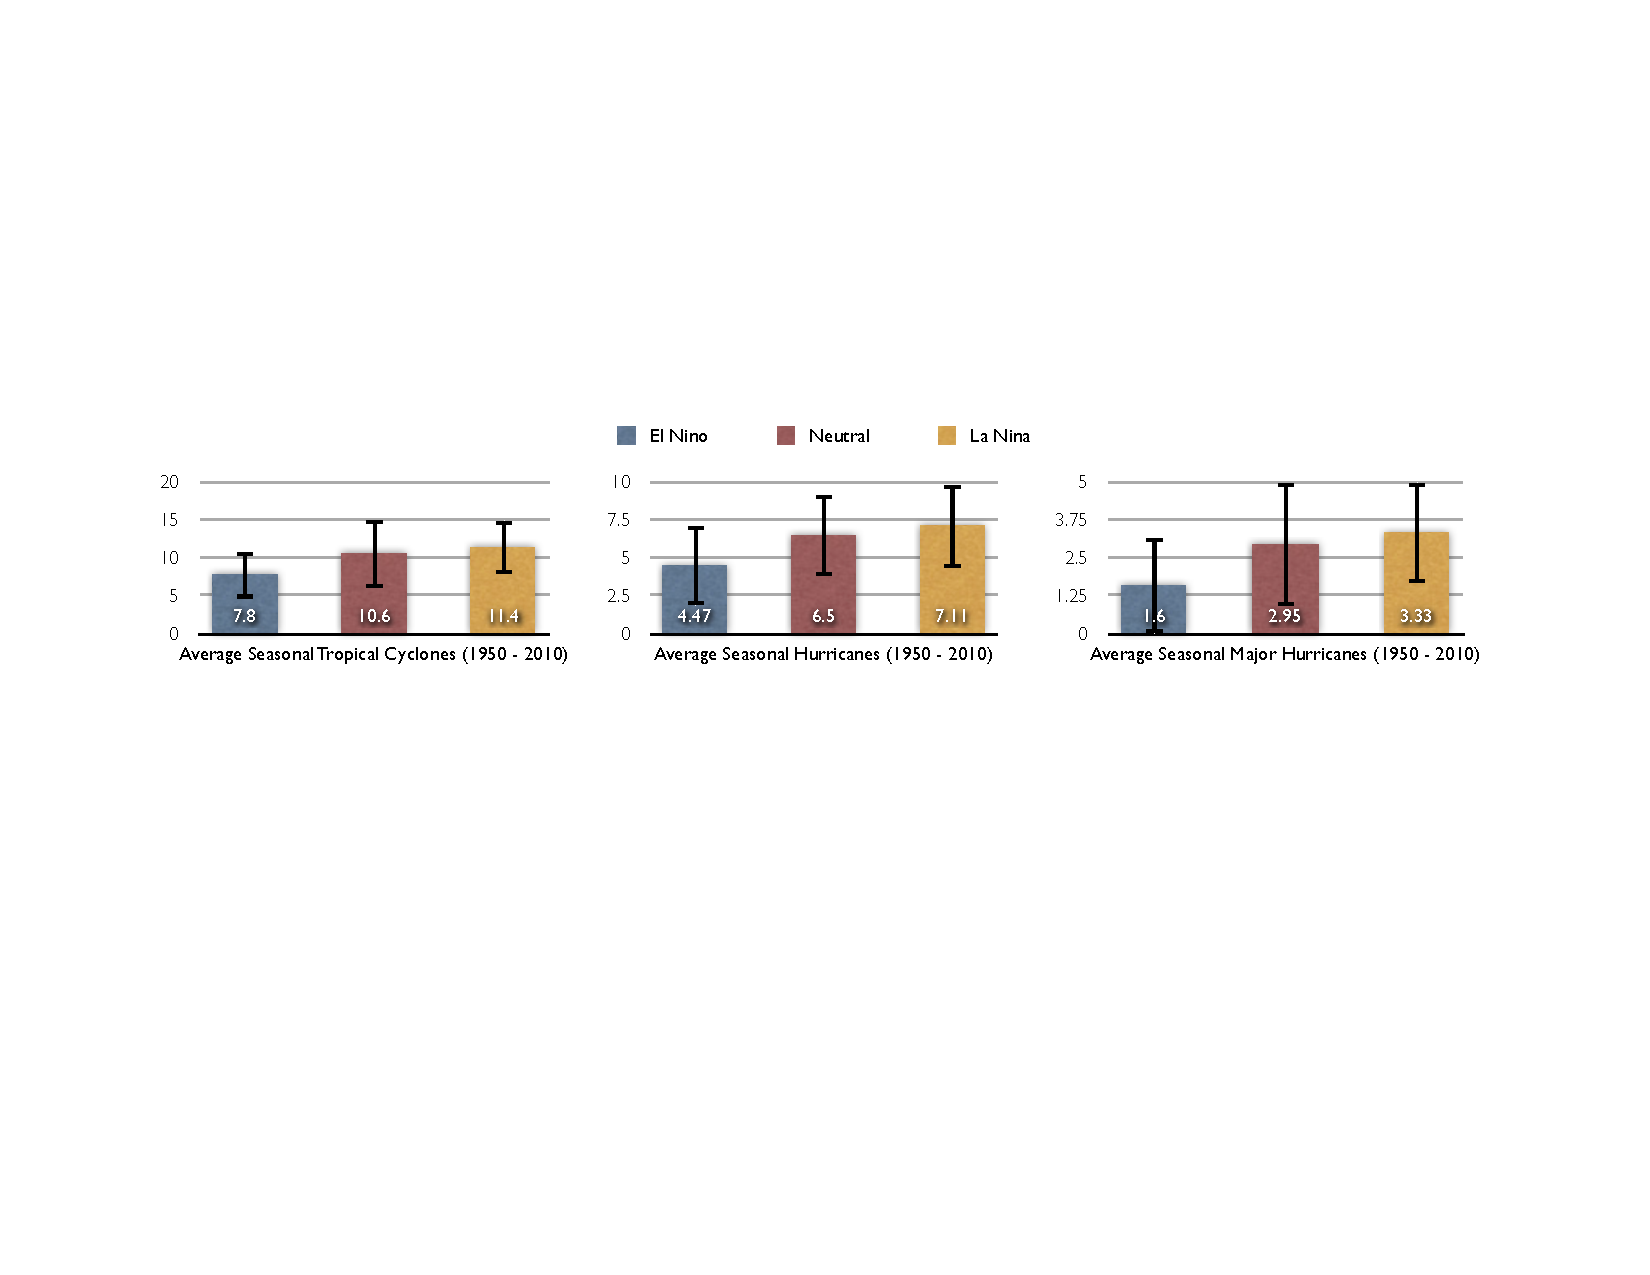
\includegraphics[height=3in]{figures/nino_nina_avg_diff.pdf}
	\caption{The $1950-2010$ seasonal mean Atlantic tropical cyclones (top), hurricanes (middle), and major hurricane (bottom) counts for El-Ni\~no, neutral, and La Ni\~na years. Vertical bars denote standard deviation. The overlap between between bars across categories make distinguishing between Atlantic TC activity based on the phase of ENSO ambiguous.}
	\label{fig:enso_bars}
\end{figure}





\subsection{ENSO Overview}
The quasi-periodic cycle (2-7 years) of warming and cooling of the near equatorial Pacific Ocean, known as the El-Ni\~no Souther Oscillation (ENSO) is associated with anomalous atmospheric circulation and alterations to the Eastern Pacific thermocline (the subsurface boundary between upper warm waters and deep cool waters). During its warm, El-Ni\~no (EN) phase, the equatorial Pacific Ocean experiences weak easterly winds causing an increase in Eastern Pacific SSTs, that in turn alters the atmospheric zonal (Walker) circulation, generally resulting in prevailing westerlies. ENSO's cold, La Ni\~na (LN) phase, is characterized by the opposite atmospheric conditions -- with cold SST anomalies along the Eastern Pacific and warm ones near the Western Pacific as a result of prevailing easterly winds (see Figure \ref{fig:enso_cartoon}). The mechanisms that control the reversal to the opposite LN phase are not fully understood \cite{kirtman1997,smith2012}. Recent research has suggested that to fully capture ENSO activity, it is no longer sufficient to monitor the warm and cold phases in the Eastern Pacific. Instead, warming patterns in the Central Pacific must be monitored as well \cite{ashok2007}. Warming in the Central Pacific, known as El Ni\~no Modoki, where a warm waters are surrounded by cold ones has been observed with increased frequency since the 1990s. Such changes have been attributed to anthropogenic global warming \cite{yeh2009} as well as natural climate variability \cite{wittenberg2009}.

Enhanced convection as a result of anomalous Pacific Ocean warming is associated with strong westerly upper tropospheric wind over the Caribbean basin and tropical Atlantic, resulting in low TC activity during EN events and high TC activity LN \cite{gray1984a}. Other studies have suggested that ENSO impact Atlantic TC activity via tropospheric warming \cite{tang2004}. 

%In fact, recent research has attributed increased accuracy in predicting seasonal TC activity with reasonable lead times to an increased ability to predict Pacific SSTs \cite{smith2010}.$

%The warming anomalies of sea surface temperatures (SSTs) along the near-equatorial Pacific Ocean have well documented global long-range weather teleconnections from rainfall in southern India to mudslides in the western United States. 

% Hurricanes, or more generally tropical cyclones (TCs), are one of the most devastating natural disasters in terms of both human and material loss. Therefore there is significant scientific and societal interest in understanding how will TC activity (frequency, intensity, and trajectories) evolve especially under global warming conditions. Our understanding our future TC activity under various warming scenarios is limited \cite{knutson2010} mainly due to two major questions: First, how will the large scale conditions over TC development regions evolve if the environment continues to warm; (ii) and if we can predict such conditions what would future TC activity be as a response to such large-scale changes? Subsequently, to understand future Atlantic TC activity, we must first understand how will the large-scale conditions over the Atlantic change and how will Atlantic TCs respond to such changes.



\begin{figure}[htbp]
	\centering
		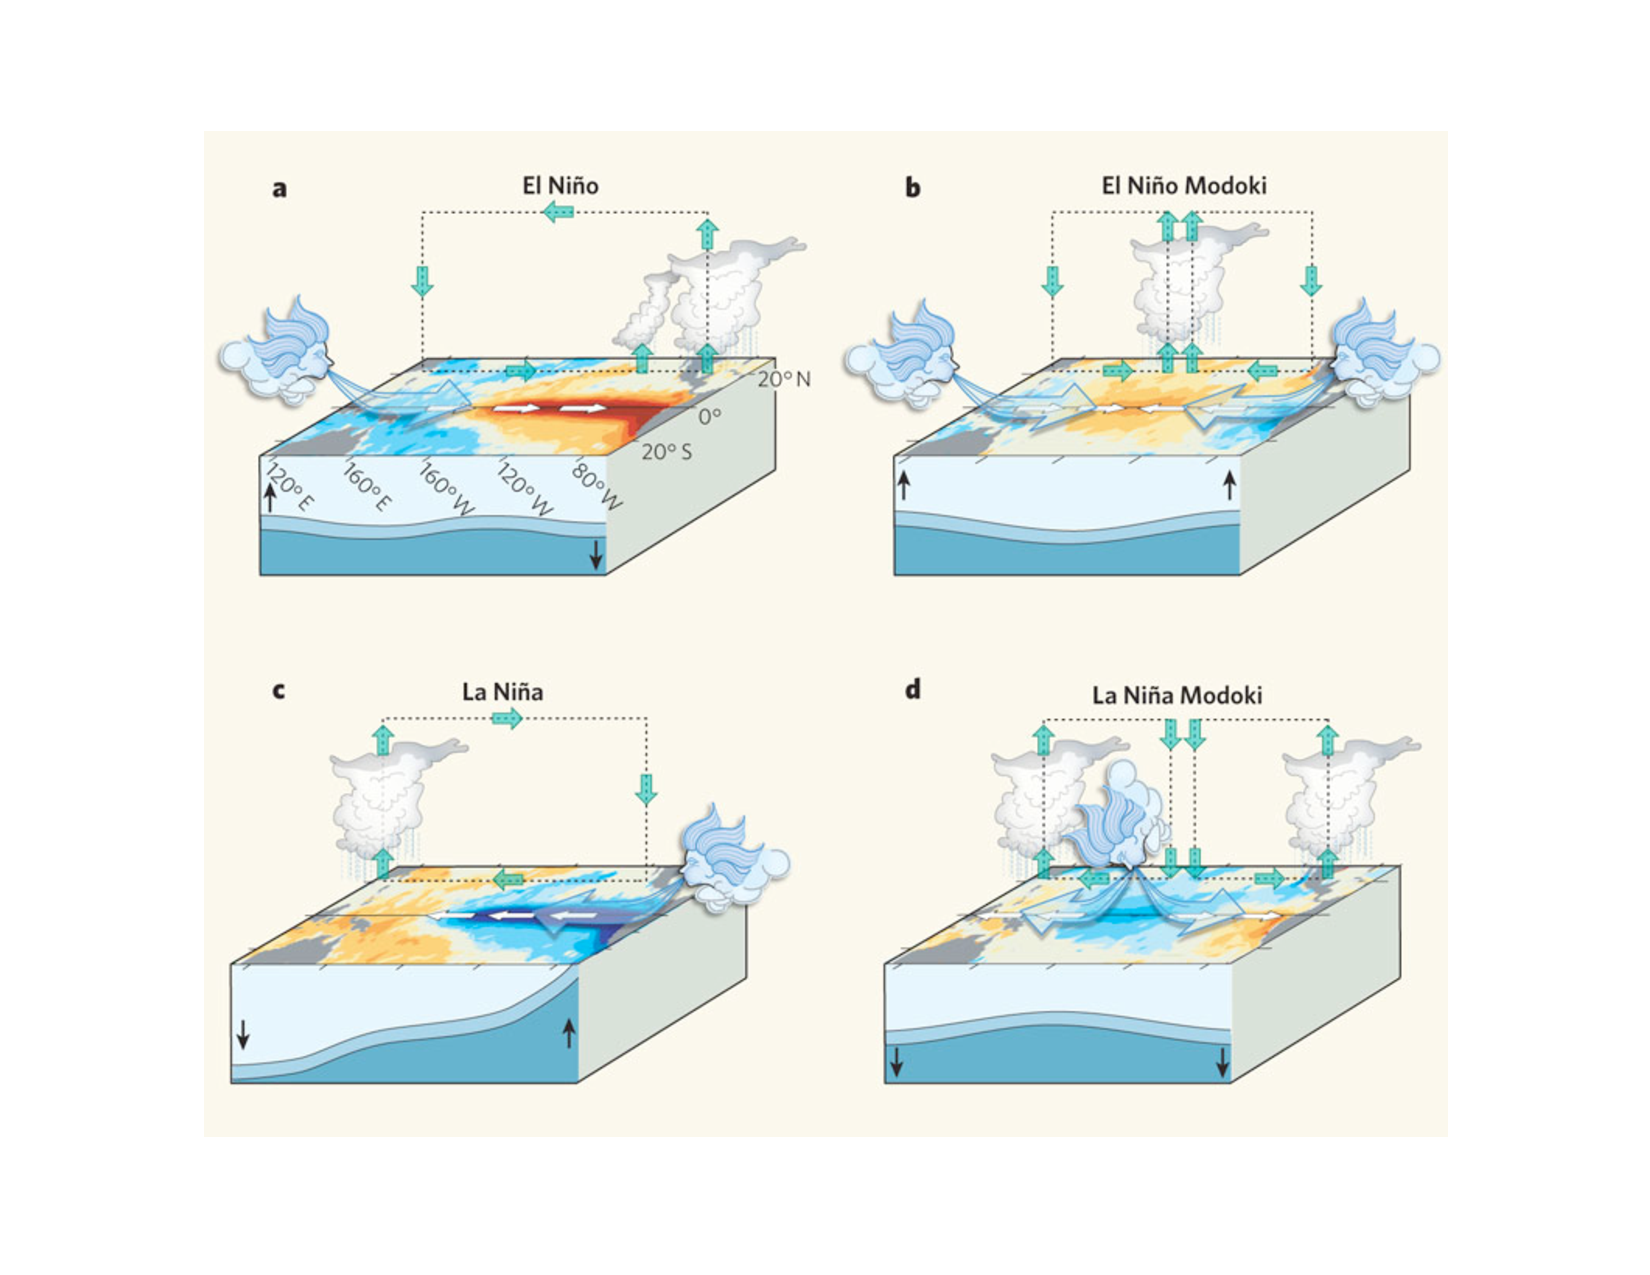
\includegraphics[height=2.5in]{figures/nino_cartoon.pdf}
	\caption{(a), An El Ni\~no event is produced when the easterly winds weaken; sometimes, in the west, westerlies prevail. This condition is categorized by warmer than normal sea surface temperatures (SSTs) in the east of the ocean, and is associated with alterations in the thermocline and in the atmospheric circulation that make the east wetter and the west drier. (b), An El Ni\~no Modoki event is an anomalous condition of a distinctly different kind. The warmest SSTs occur in the central Pacific, flanked by colder waters to the east and west, and are associated with distinct patterns of atmospheric convection. (c), (d), The opposite (La Ni\~na) phases of the El Niño and El Ni\~no Modoki respectively. Image and caption used for illustration purposes only taken from \cite{ashok2009}}
	\label{fig:enso_cartoon}
\end{figure}



%Given its long-range teleconnections, as well as ENSO being the most dominant feature of cyclic climate variability on subdecadal timescales, effectively abstracting and predicting Pacific Ocean warming anomalies has been a subject of active research. 


\section{Spatial ENSO Index (S-ENSO)}
An increasing number of studies have suggested changes in the spatial warming patterns of the Pacific Ocean and some have linked those changes U.S. hurricane landfall probabilities \cite{kim2009}. We propose that based on such results, the spatial distribution of Pacific Ocean warming might provide better predictive insights into ENSO-Atlantic TC activity than warming anomalies alone. We propose a distance-based ENSO index that tracks the location of maximum near-tropical Pacific warming anomaly (Pacific Warm Pool or PWP thereafter) instead of its absolute warming.

For each season, we search for the maximum positive warming anomaly in regions of size comparable to that of warming-based ENSO indices. The PWP is selected by searching the Northern Tropical Pacific ($0-30^\circ$ N). The time series of the longitude of the PWP is then correlated with various quantities that communicate August-October Atlantic TC activity: number of tropical cyclones, number of major hurricanes, potential dissipation index (PDI) \cite{emanuel2005a}, accumulated cyclone energy (ACE) \cite{Bell2000}, and net tropical cyclone energy (NTC) \cite{goldenberg2001}.

In addition to tracking the longitude of the PWP, we also monitored other environmental factors that might influence Atlantic TC activity: the mean pressure value over the PWP, the mean Outgoing Longwave Radiation (OLR) of the PWP to monitor atmospheric deep convection, the longitude of the minimal pressure region to approximate Pacific cyclone activity, and finally the longitudinal distance between PWP and the coldest near equatorial Pacific SST region (Pacific Cold Pool or PCP). Finally, we ran a series of exhaustive experiments to linearly combine the above mentioned quantities into a single index (named Combo Index). Each index is built by computing the z-score for each quantity (i.e. mean OLR, etc.) then we add each normalized quantity to build a single index to use for analysis. Please see table \ref{table:acronyms}

\begin{table}
\begin{tabular}{cc}
\hline
Acronym & Quantity\\
\hline
PWP-Lon & The longitude of the warmest SST pool in the northern near equatorial Pacific\\
PWP-Pres & The mean presure of PWP\\
PWP-OLR &  The mean OLR of PWP \\
MinPres-Lon & The longitude of the region with the lowest mean central pressure\\
PWP-PCP & The longitudinal distance between PWP and PCP \\
Combo Index & A linear combination of xxxx \\
\hline
\end{tabular}
\caption{A List of all quantities computed for this study with their corresponding acronyms.}
\label{ref:acronyms}
\end{table}


Tables \ref{table:april_lead} through \ref{table:oct_lead} show the linear correlation coefficients between August-October TC Atlantic TC activity and our ENSO spatial index for Feb-April, April-June, and August-October respectively. In all cases our spatial ENSO index correlates better than traditional warming-based indices. The improvements increase as we increase lead time, with April lead times improving by more than an order of magnitude. This improvement is because traditional ENSO indices suffer from a ``predictability barrier" that make it difficult to use them to predict TC activity before June \cite{webster1992}.




% \begin{table}
% \begin{center}
% \begin{tabular}{cccccc}
% \hline
% &TCs & Major Hurricanes & ACE & PDI & NTC\\
% \hline
% Spatial ENSO & -0.44 & -0.39 & -0.40 & -0.39 & -0.43\\
% NINO 1+2 & -0.07 & -0.13 & 0.01 & 0.02 & -0.04\\
% NINO 3.4 & -0.07 & -0.11 & 0.01 & 0.02 & 0.03\\
% NINO 3 & 0.04 & -0.08 & 0.06 & 0.08 & 0.03\\
% NINO 4 & 0.09 & -0.08 & 0.08 & 0.11 & 0.10\\
% \hline
% \end{tabular}
% \end{center}
% \caption{Linear correlation coefficients between January-April mean SSTs of traditional warming-based ENSO indices as well as the January-April Spatial ENSO index and August-October Atlantic TC activity. Our Spatial ENSO index significantly outperforms traditional indices.}
% \label{ref:table_jan_apl_corr}
% \end{table}
% 
% \begin{table}
% \begin{center}
% \begin{tabular}{cccccc}
% \hline
% &TCs & Major Hurricanes & ACE & PDI & NTC\\
% \hline
% Spatial ENSO & -0.53 & -0.48 & -0.36 & -0.34 & -0.40\\
% NINO 1+2 & -0.23 & -0.32 & -0.25 & -0.26 & -0.28\\
% NINO 3.4 & -0.23 & -0.44 & -0.25 & -0.26 & -0.29\\
% NINO 3 & -0.28 & -0.40 & -0.28 & -0.29 & -0.31\\
% NINO 4 & -0.10 & -0.27 & -0.10 & -0.08 & -0.09\\
% \hline
% \end{tabular}
% \end{center}
% \caption{Linear correlation coefficients between April-June mean SSTs of traditional warming-based ENSO indices as well as the January-April Spatial ENSO index and August-October Atlantic TC activity. Our Spatial ENSO index significantly outperforms traditional indices.}
% \label{ref:table_apr_jun}
% \end{table}
% 
% \begin{table}
% \begin{center}
% \begin{tabular}{cccccc}
% \hline
% &TCs & Major Hurricanes & ACE & PDI & NTC\\
% \hline
% Spatial ENSO & -0.62 & -0.57 & -0.69 & -0.67 & -0.70\\
% NINO 1+2 & -0.55 & -0.47 & -0.44 & -0.42 & -0.49\\
% NINO 3.4 & -0.55 & -0.51 & -0.44 & -0.42 & -0.46\\
% NINO 3 & -0.51 & -0.50 & -0.46 & -0.44 & -0.49\\
% NINO 4 & -0.34 & -0.48 & -0.33 & -0.32 & -0.35\\
% \hline
% \end{tabular}
% \end{center}
% \caption{Linear correlation coefficients between July-October mean SSTs of traditional warming-based ENSO indices as well as the January-April Spatial ENSO index and August-October Atlantic TC activity. Our Spatial ENSO index significantly outperforms traditional indices.}
% \label{ref:table_jul_oct}
% \end{table}

\subsection{Sensitivity Tests}
To validate our results, we test the sensitivity of our results to the month ranges used to build the index, the size of the ENSO box used, the size of the search space, and the months used as TC season. As it can be seen from the figures below, our results are stable with respect to parameter choice, except for search space where the correlations chance drastically based on which region we search.
%\pagebreak
\subsection{Box Size Sensitivity Results}
\begin{figure}[ht]
\begin{minipage}[b]{0.6\linewidth}
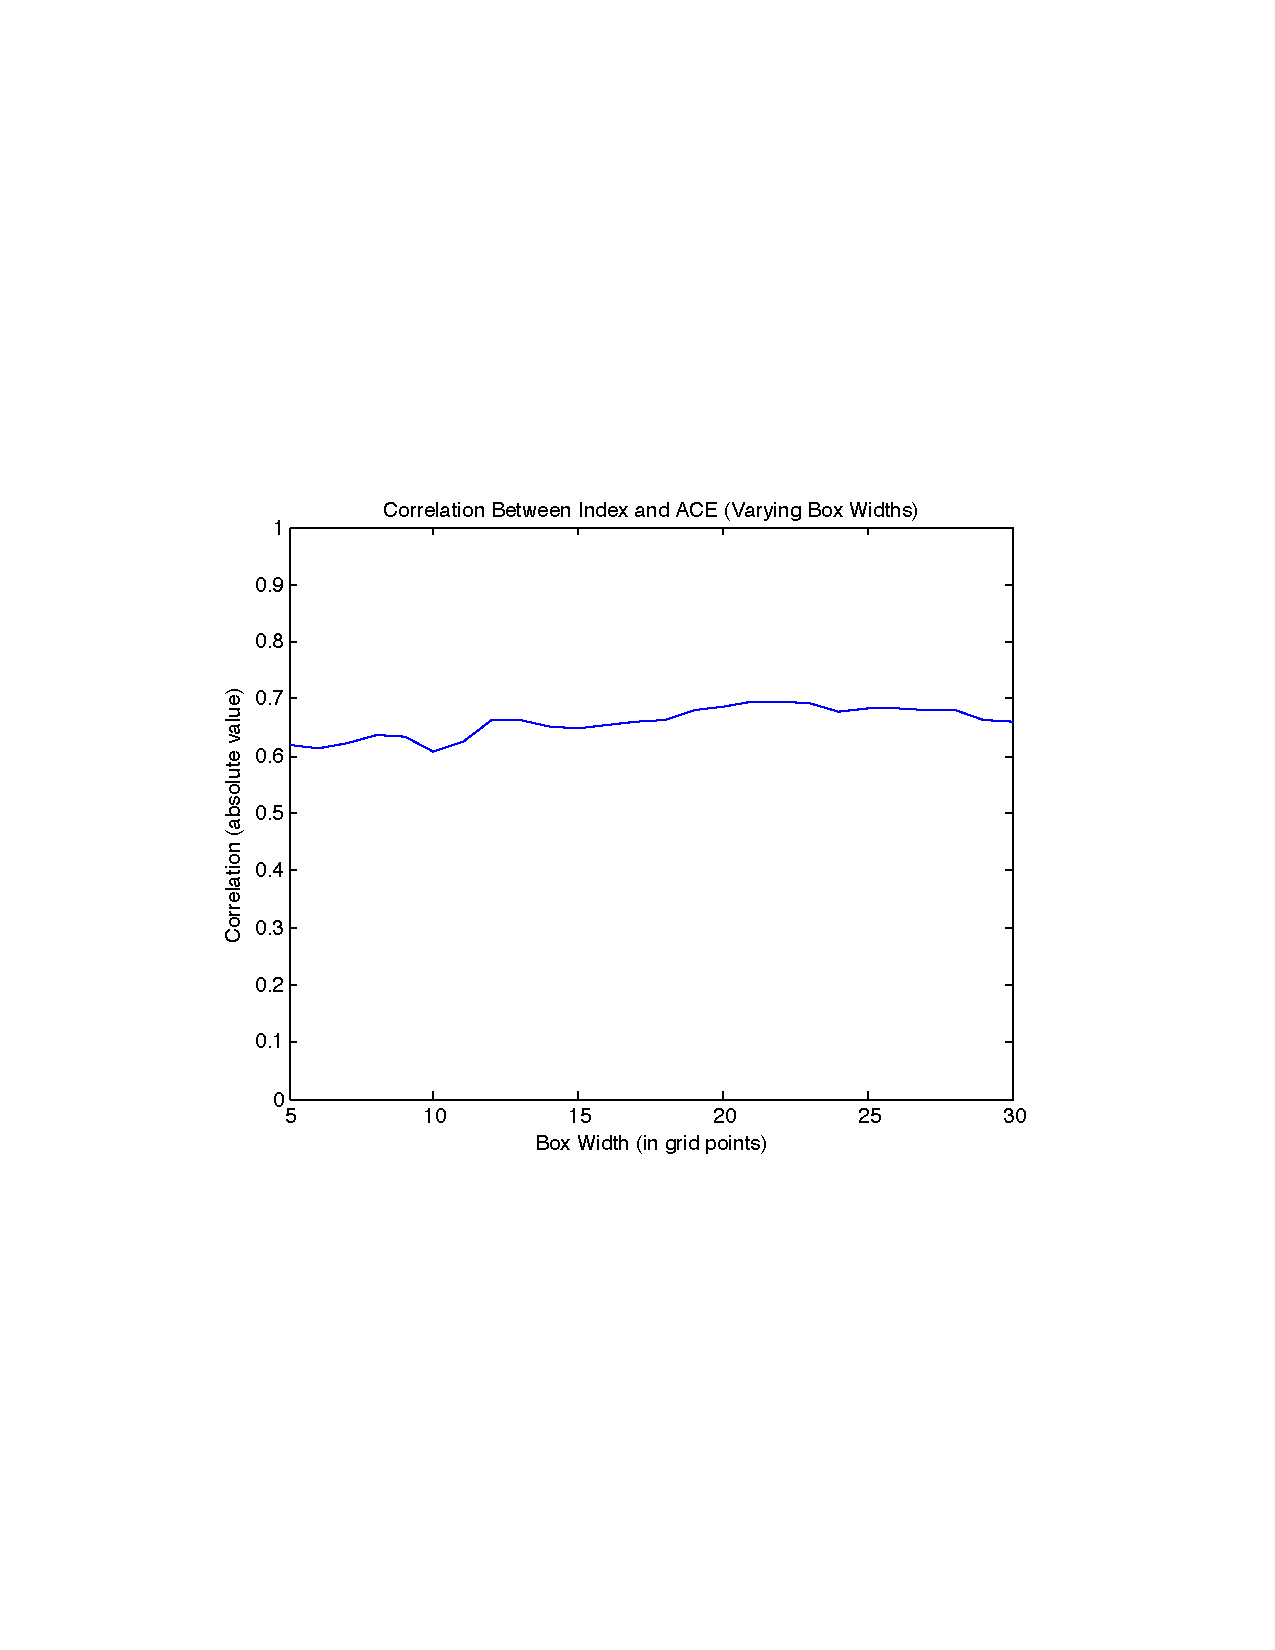
\includegraphics[width=\textwidth]{figures/sensitivityResults/boxSize/ACE_Index_Box_Size.pdf}
\caption{Corr Index vs. ACE}
\label{fig:figure1}
\end{minipage}
\hspace{0cm}
\begin{minipage}[b]{0.6\linewidth}
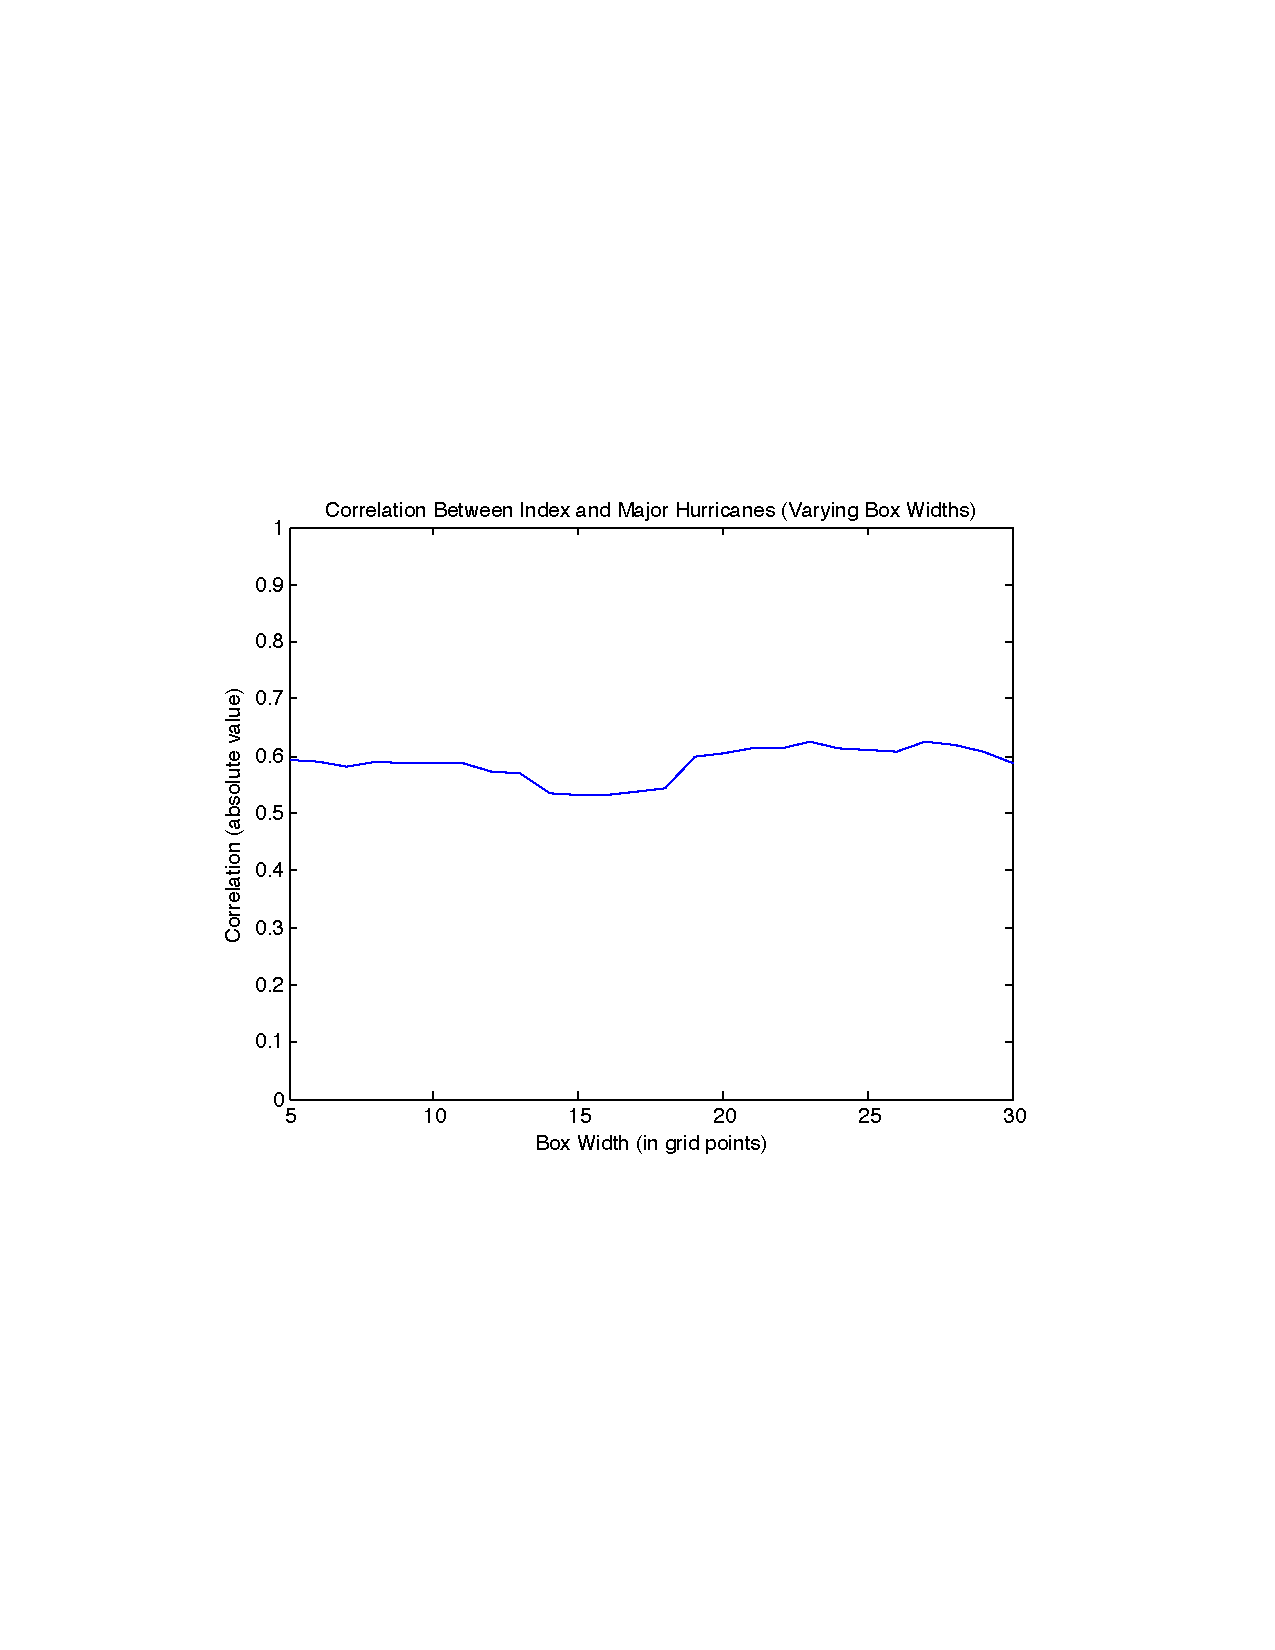
\includegraphics[width=\textwidth]{figures/sensitivityResults/boxSize/Major_Hurricanes_Index_Box_Size.pdf}
\caption{Corr Index vs. Major Hurricanes}
\label{fig:figure2}
\end{minipage}
\end{figure}
\begin{figure}[ht]
\begin{minipage}[b]{0.6\linewidth}
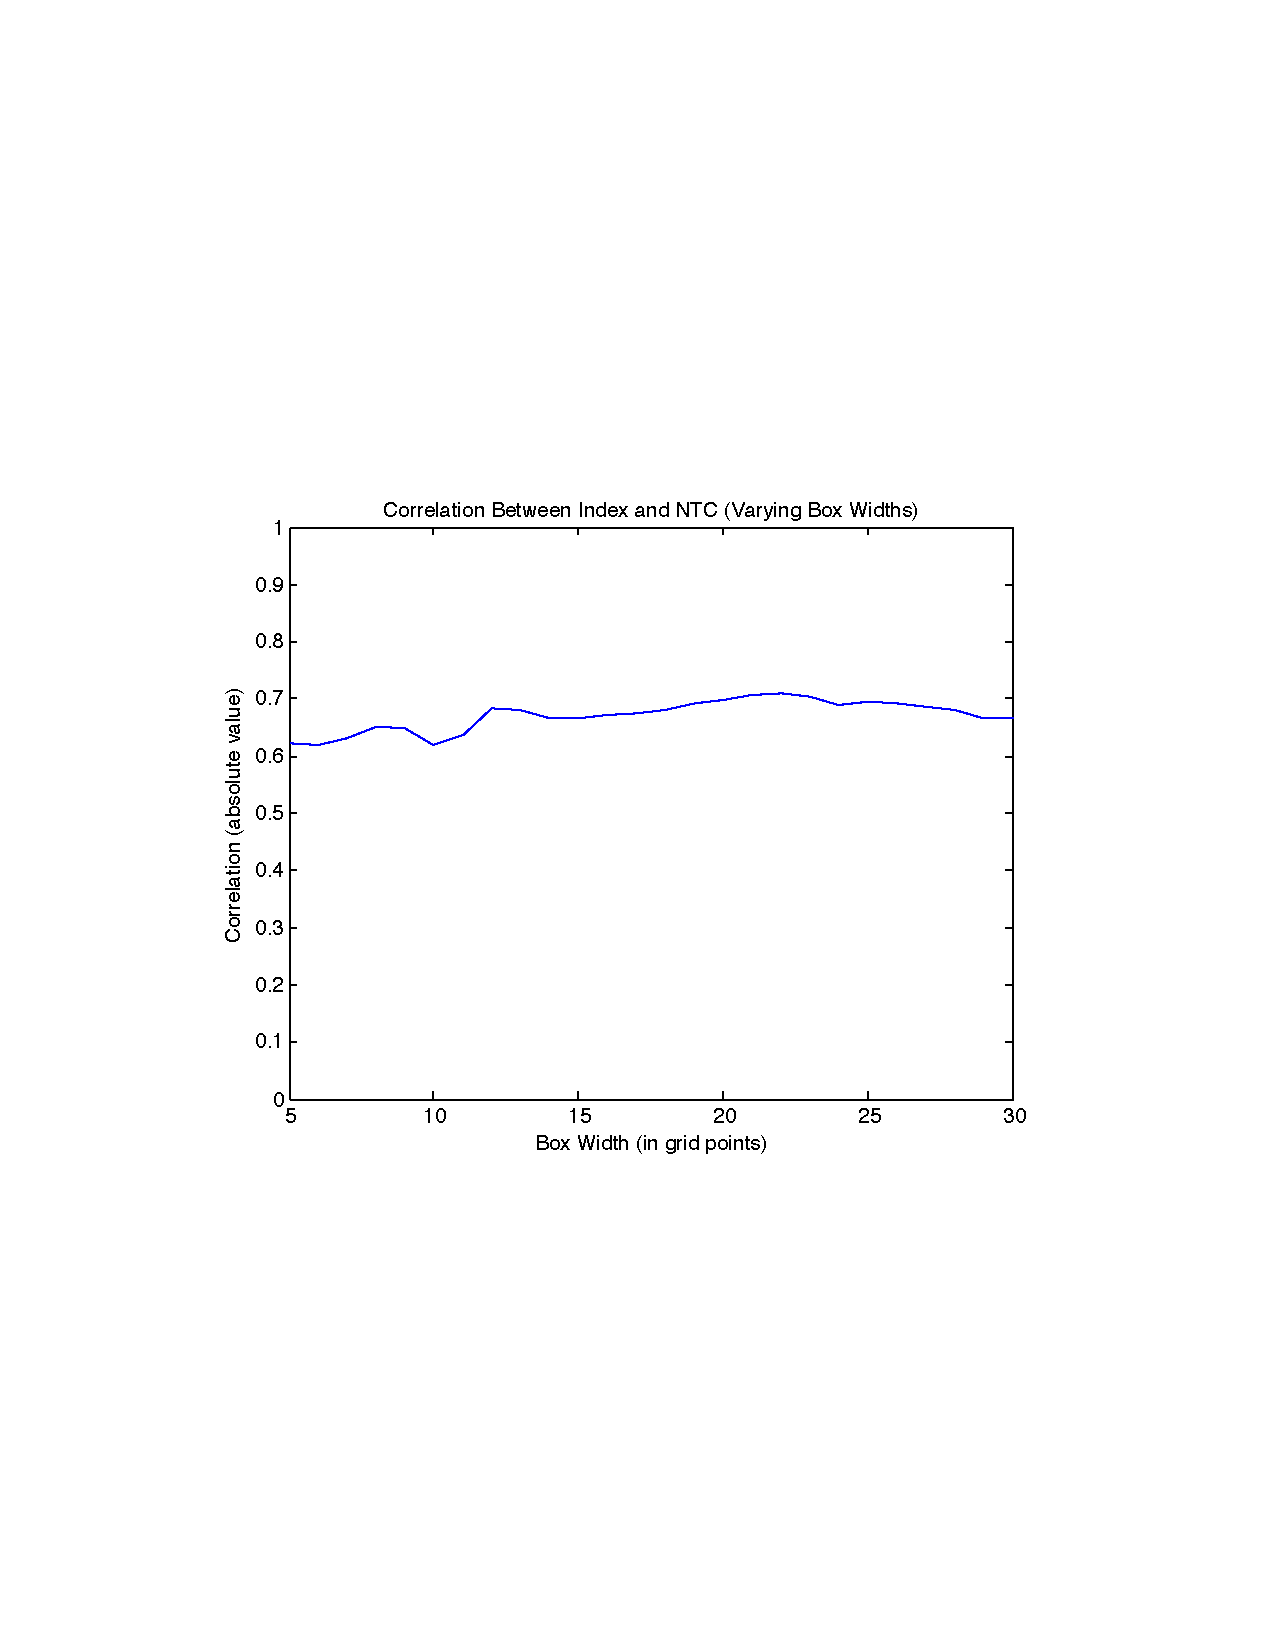
\includegraphics[width=\textwidth]{figures/sensitivityResults/boxSize/NTC_Index_Box_Size.pdf}
\caption{Corr Index vs. NTC}
\label{fig:figure3}
\end{minipage}
\hspace{0cm}
\begin{minipage}[b]{0.6\linewidth}
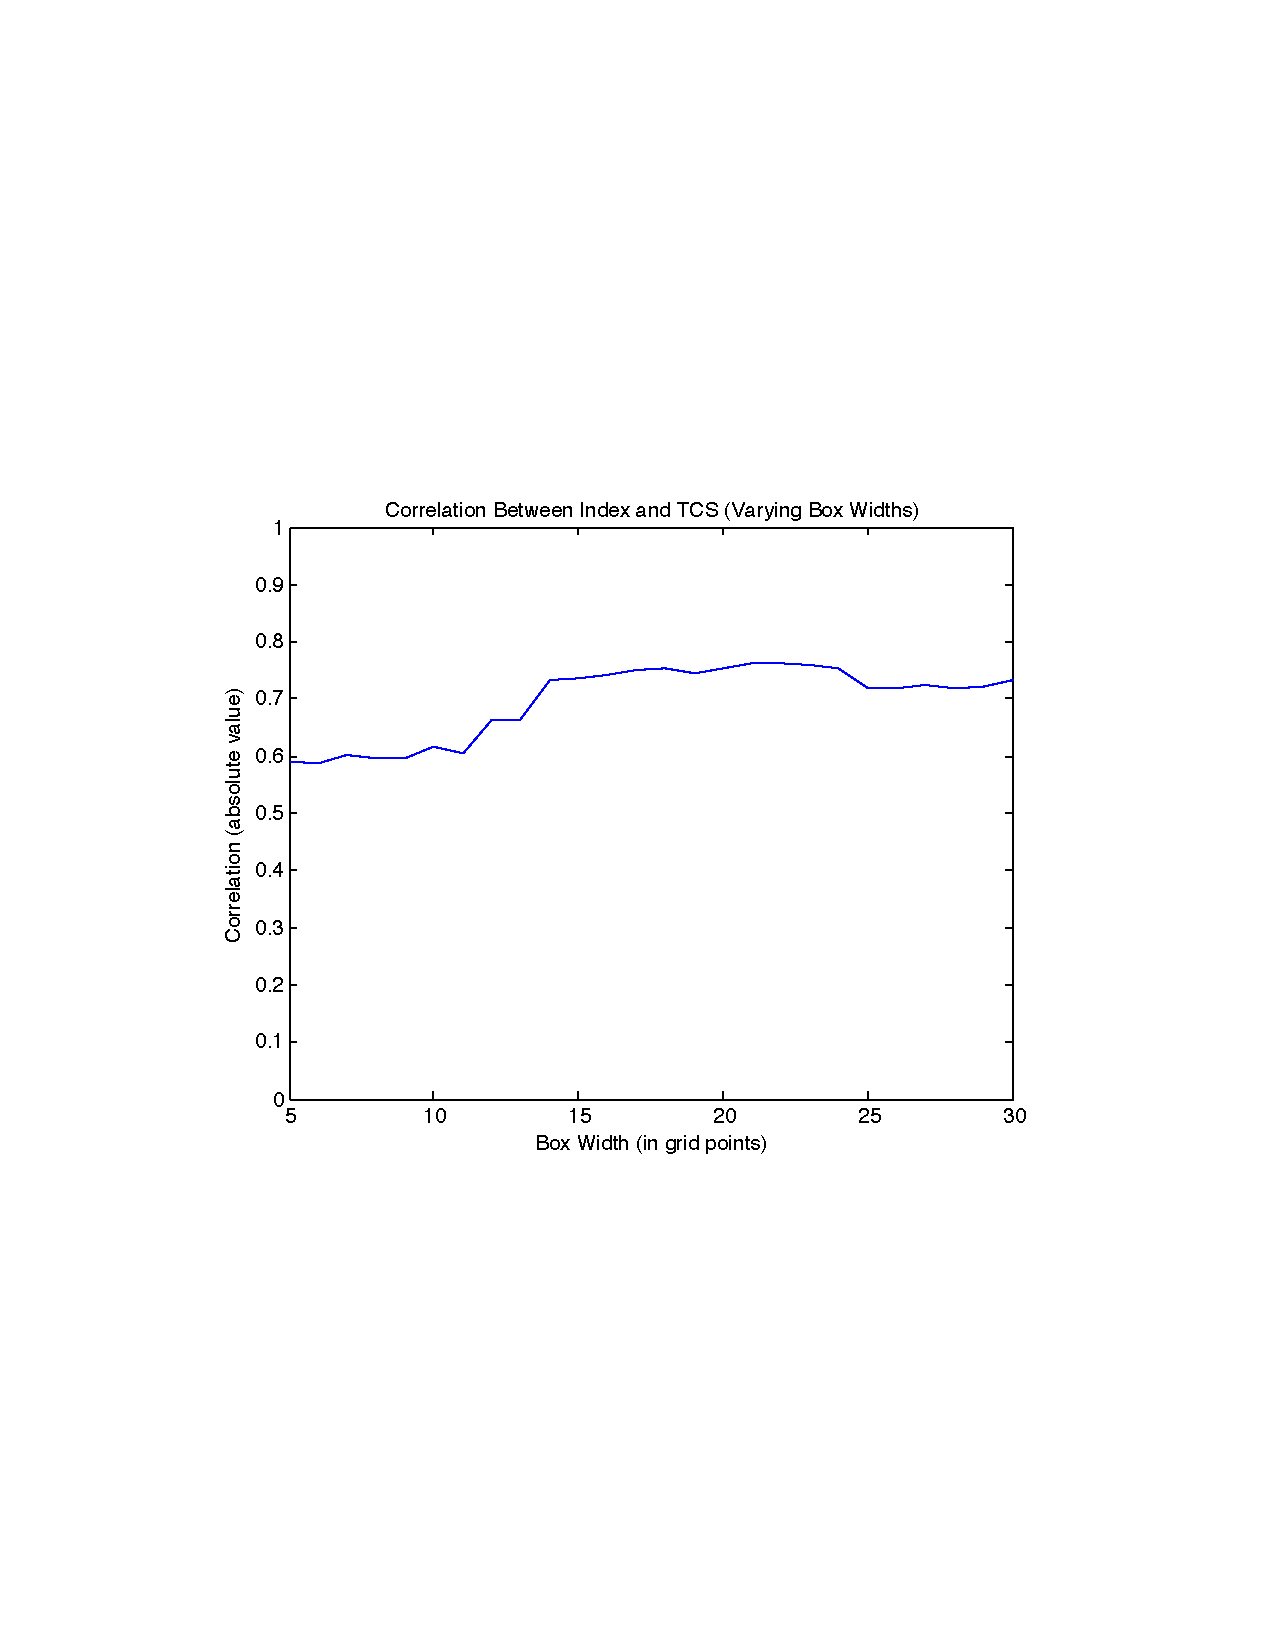
\includegraphics[width=\textwidth]{figures/sensitivityResults/boxSize/TCS_Index_Box_Size.pdf}
\caption{Corr Index vs. TCs}
\label{fig:figure4}
\end{minipage}
\end{figure}
\pagebreak
\subsection{Varying Month Ranges}

\begin{figure}[ht]
\begin{minipage}[b]{0.6\linewidth}
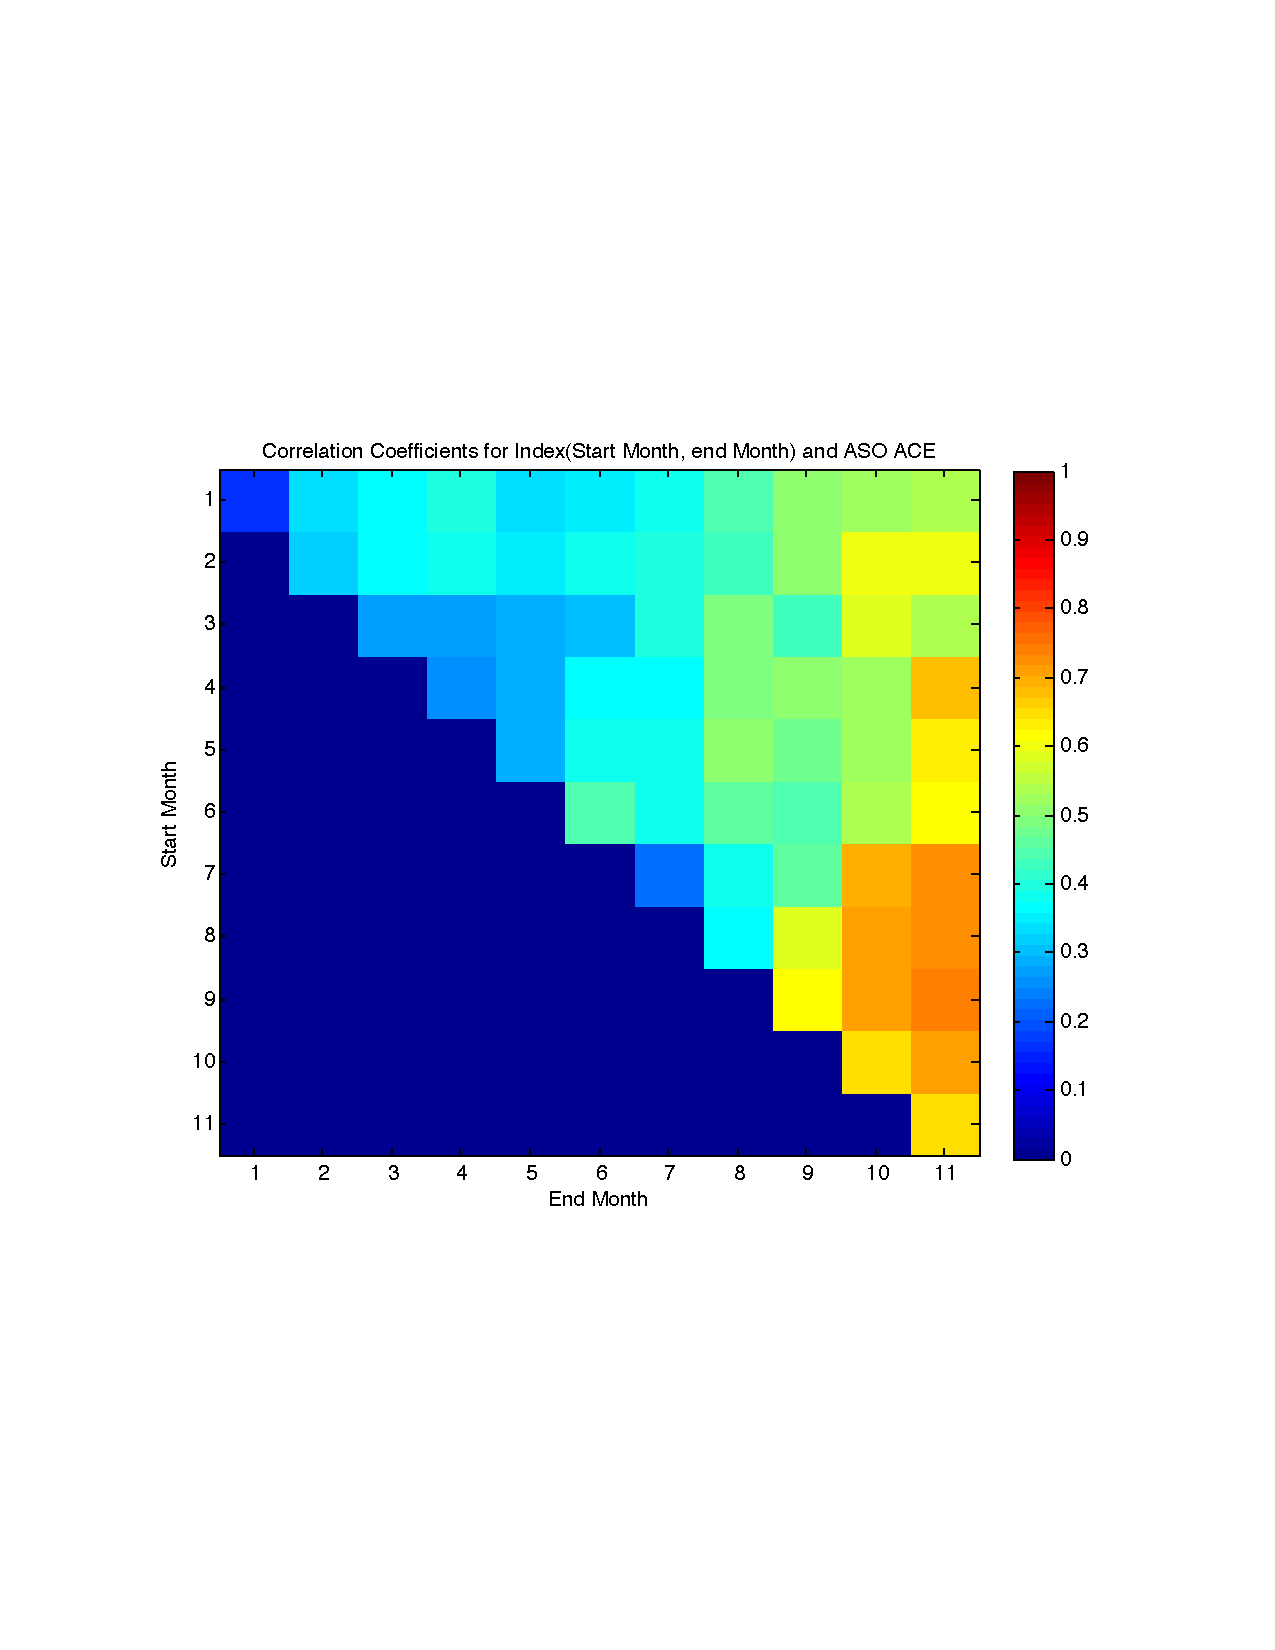
\includegraphics[width=\textwidth]{figures/sensitivityResults/monthRanges/index_corr_month_ranges_ace_month_range.pdf}
\caption{Corr Index vs. ACE}
\label{fig:figure5}
\end{minipage}
\hspace{0cm}
\begin{minipage}[b]{0.6\linewidth}
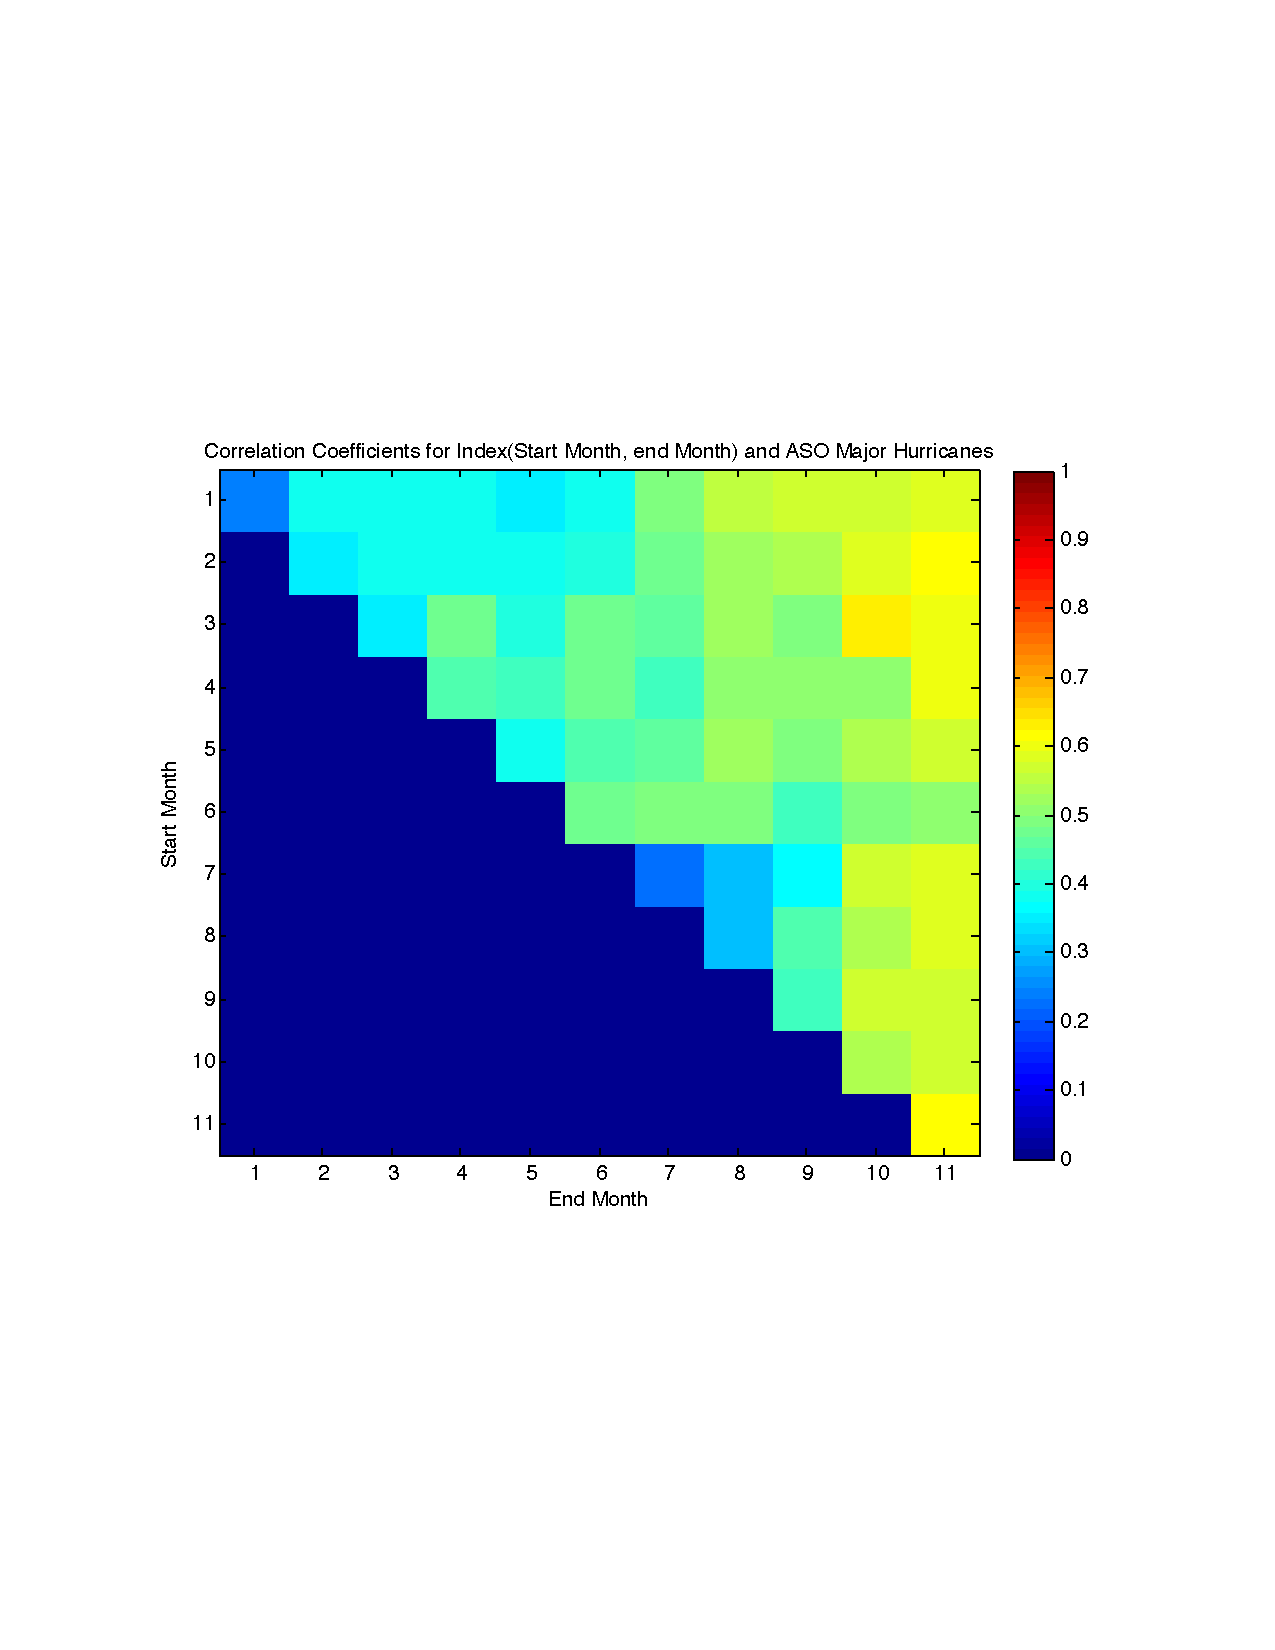
\includegraphics[width=\textwidth]{figures/sensitivityResults/monthRanges/index_corr_month_ranges_hurr_month_range.pdf}
\caption{Corr Index vs. Major Hurricanes}
\label{fig:figure6}
\end{minipage}
\end{figure}

\begin{figure}[ht]
\begin{minipage}[b]{0.6\linewidth}
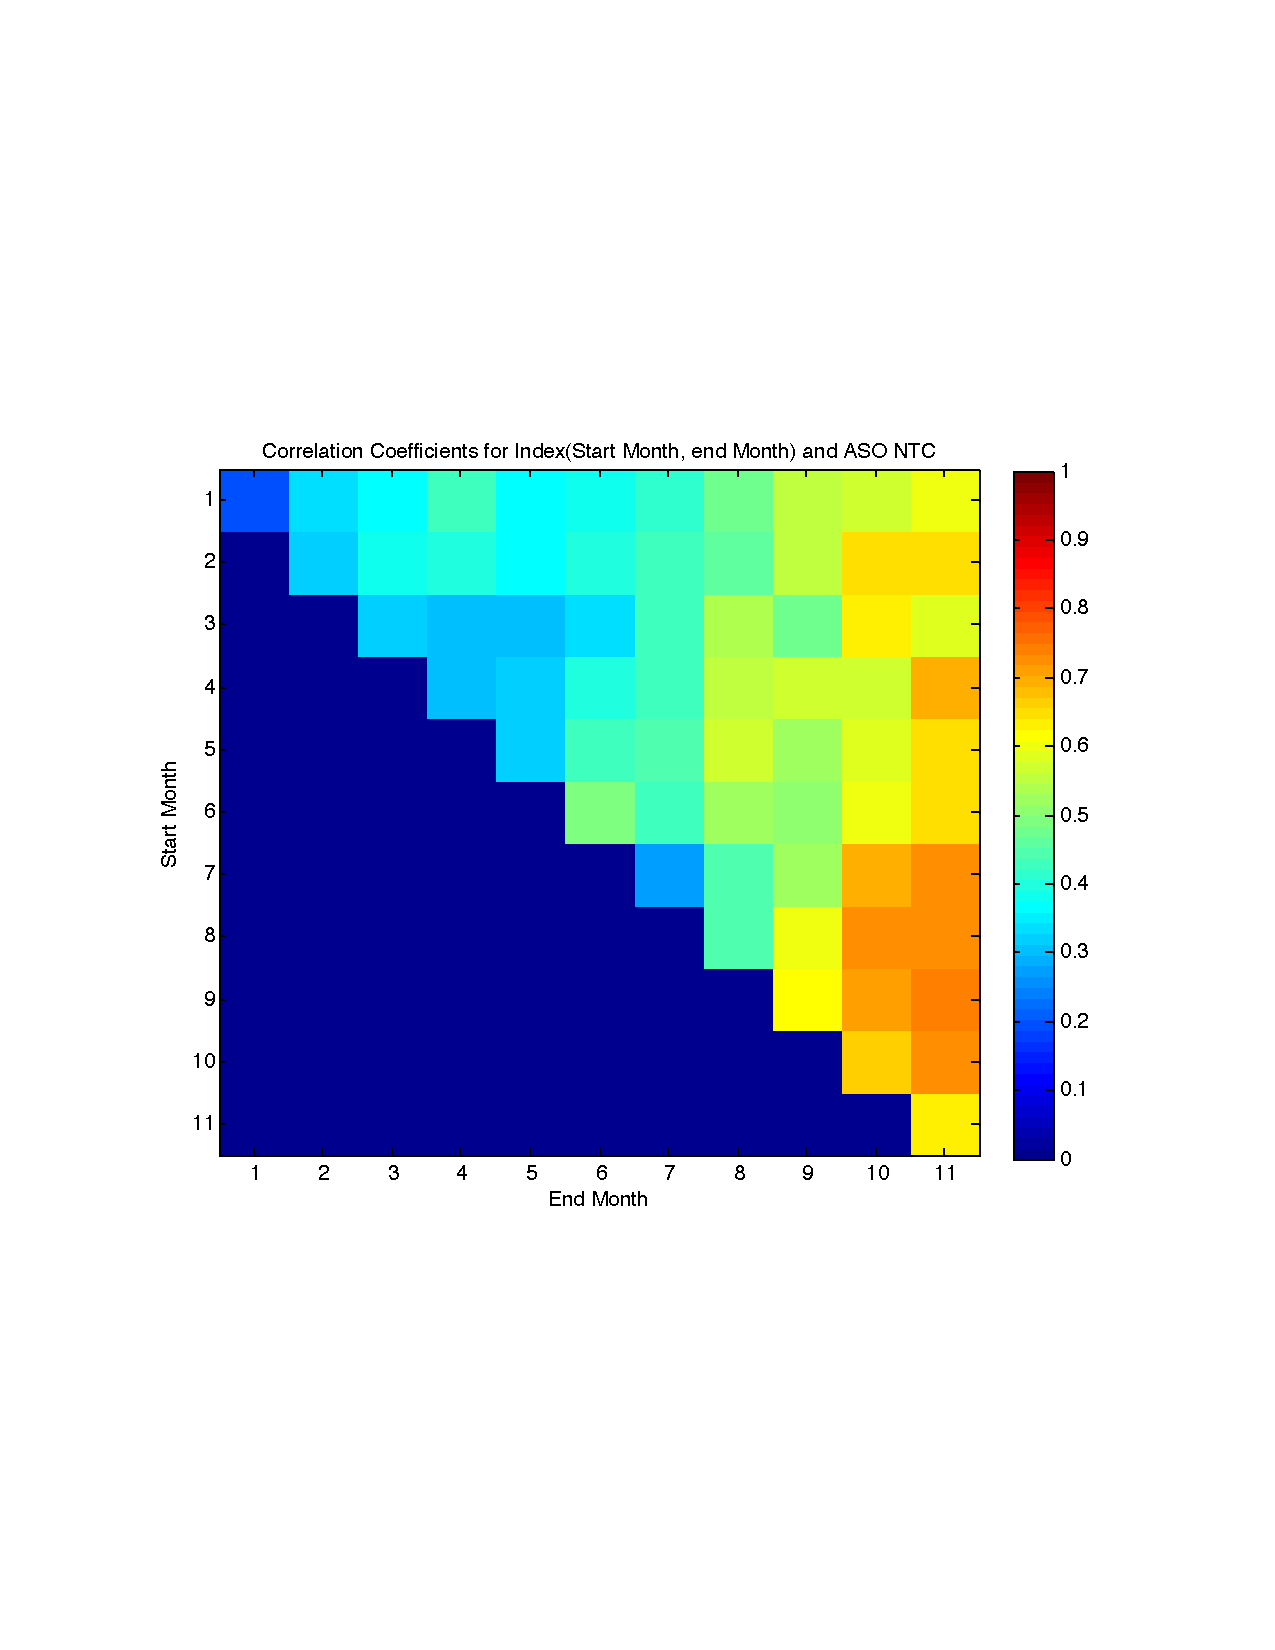
\includegraphics[width=\textwidth]{figures/sensitivityResults/monthRanges/index_corr_month_ranges_ntc_month_range.pdf}
\caption{Corr Index vs. NTC}
\label{fig:figure7}
\end{minipage}
\hspace{0cm}
\begin{minipage}[b]{0.6\linewidth}
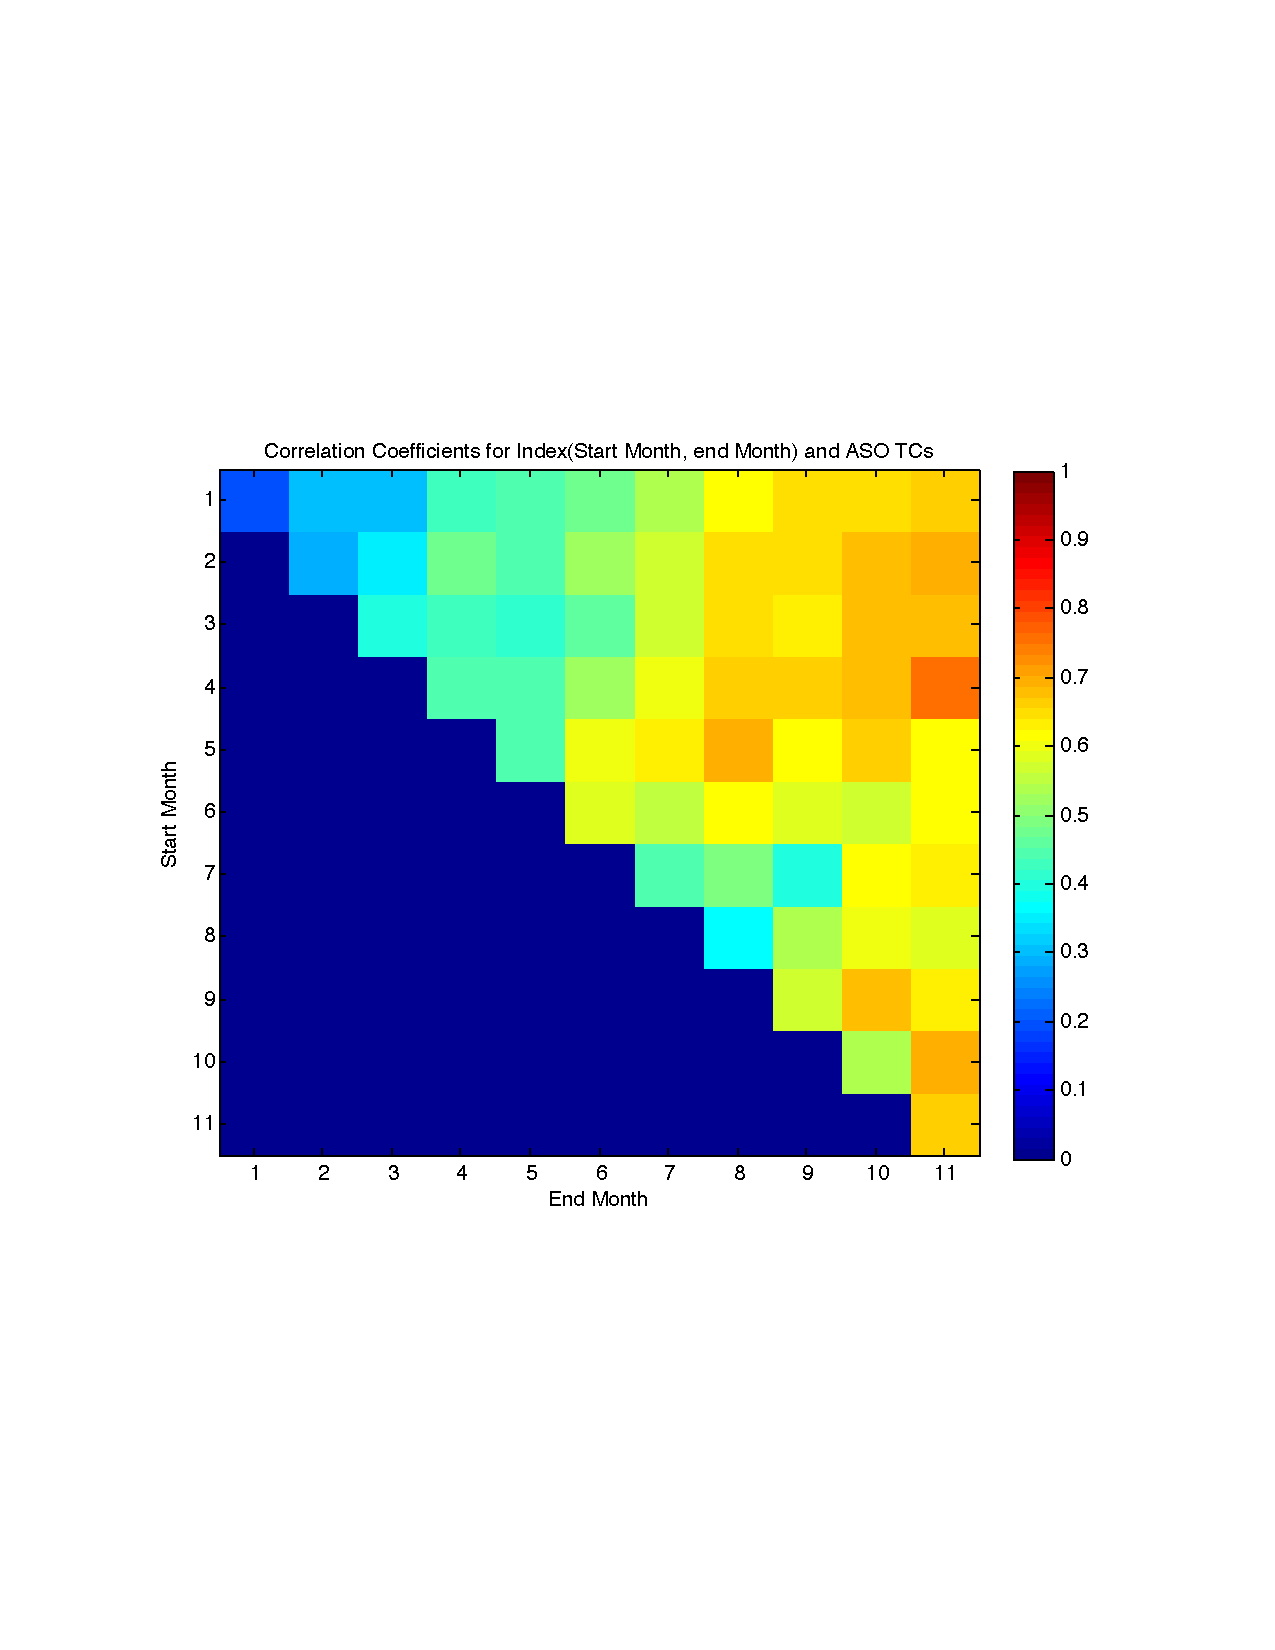
\includegraphics[width=\textwidth]{figures/sensitivityResults/monthRanges/index_corr_month_ranges_tcs_month_range.pdf}
\caption{Corr Index vs. TCs}
\label{fig:figure8}
\end{minipage}
\end{figure}

\pagebreak
\subsection{Varying Search Space (North and South Hemispheres)}
\begin{figure}[ht]
\begin{minipage}[b]{0.6\linewidth}
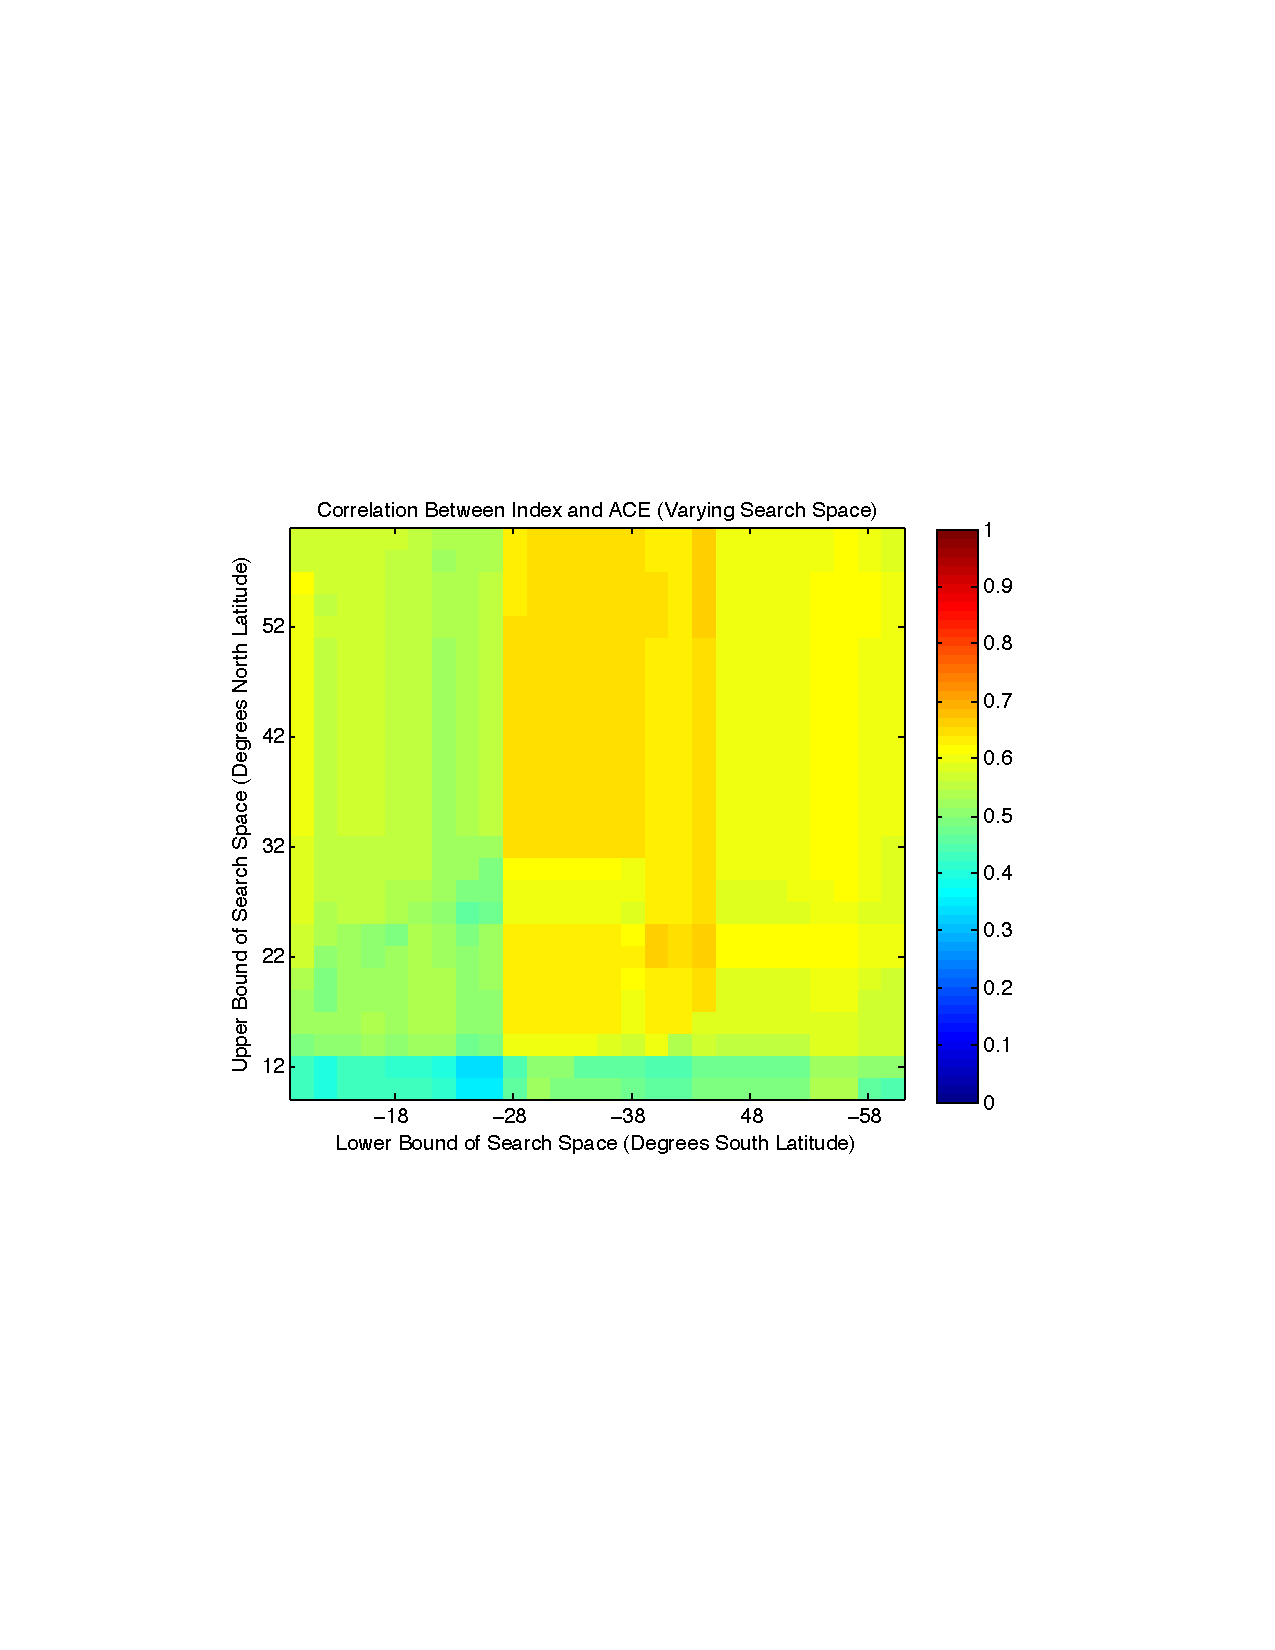
\includegraphics[width=\textwidth]{figures/sensitivityResults/northSouthHem/ACE_Index_North_South.pdf}
\caption{Corr Index vs. ACE}
\label{fig:figure9}
\end{minipage}
\hspace{0cm}
\begin{minipage}[b]{0.6\linewidth}
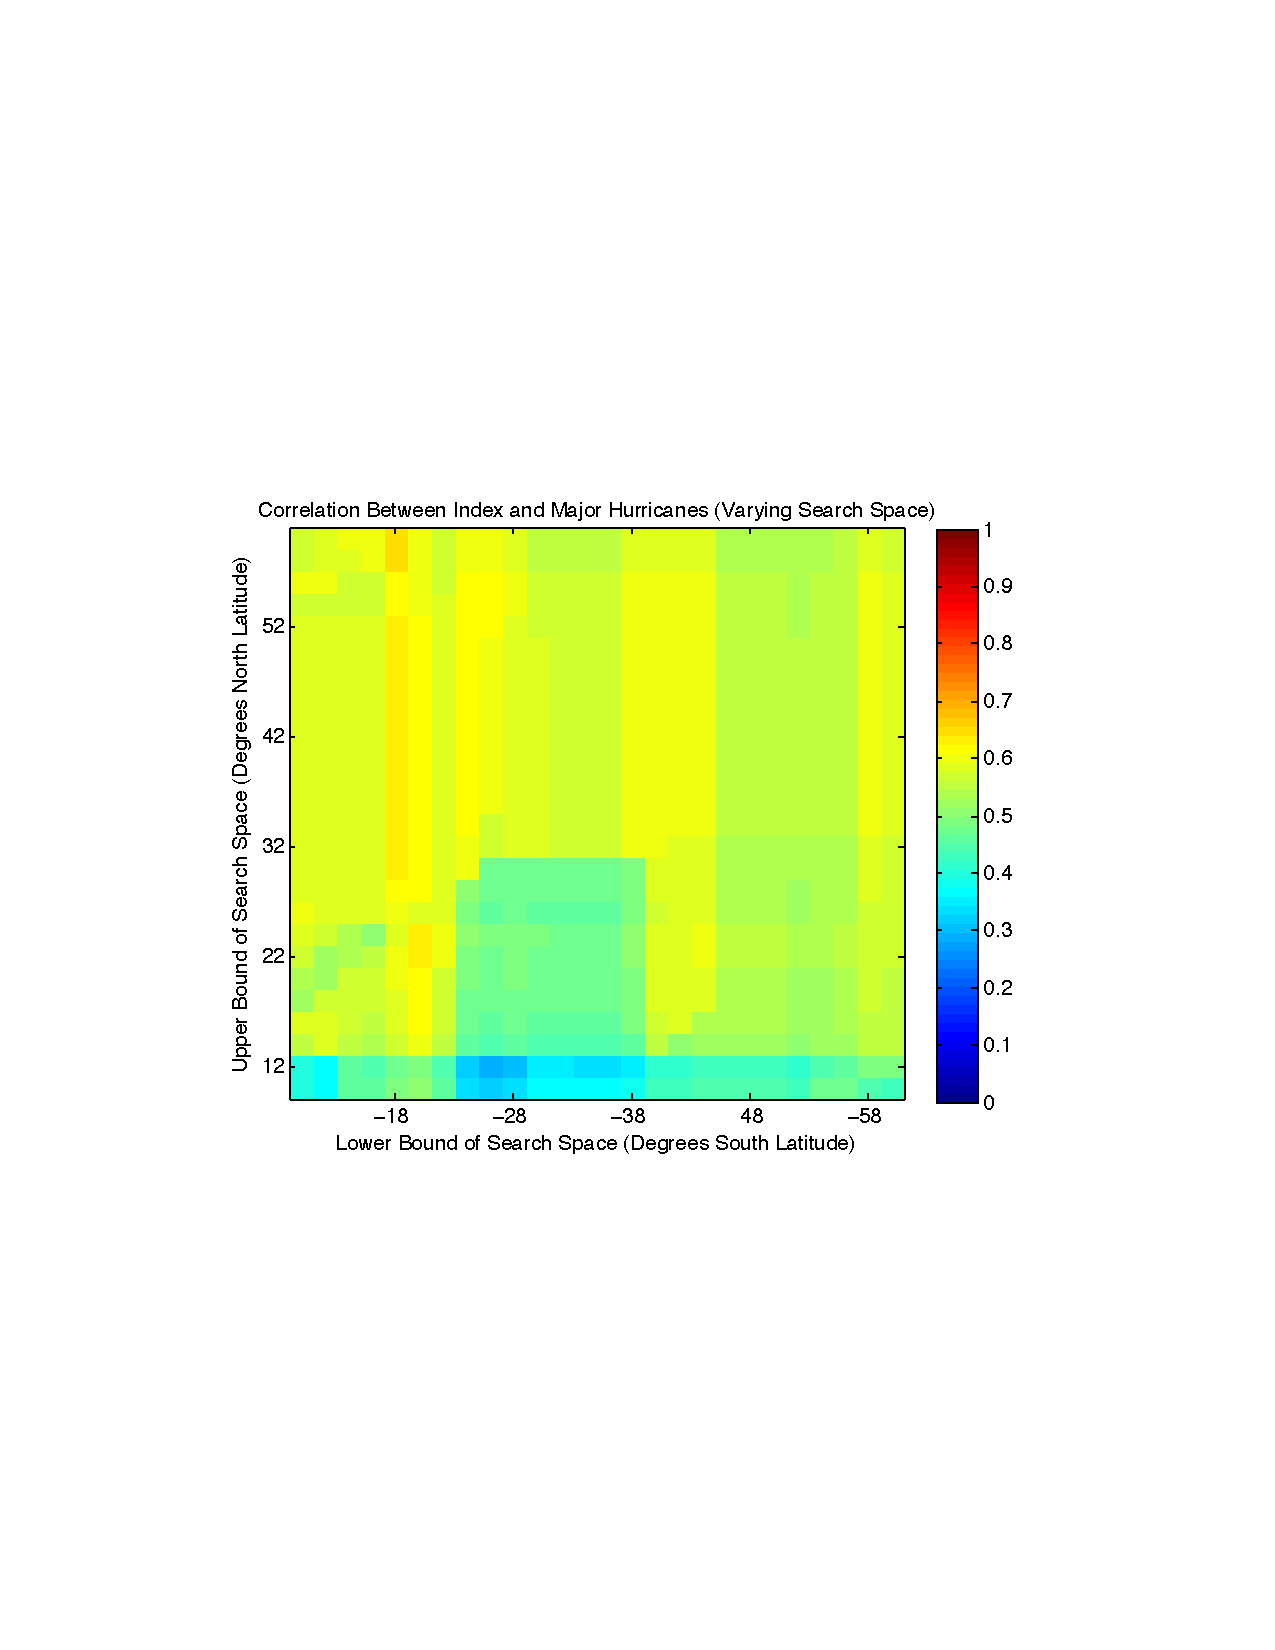
\includegraphics[width=\textwidth]{figures/sensitivityResults/northSouthHem/Major_Hurricanes_Index_North_South.pdf}
\caption{Corr Index vs. Major Hurricanes}
\label{fig:figure10}
\end{minipage}
\end{figure}

\begin{figure}[ht]
\begin{minipage}[b]{0.6\linewidth}
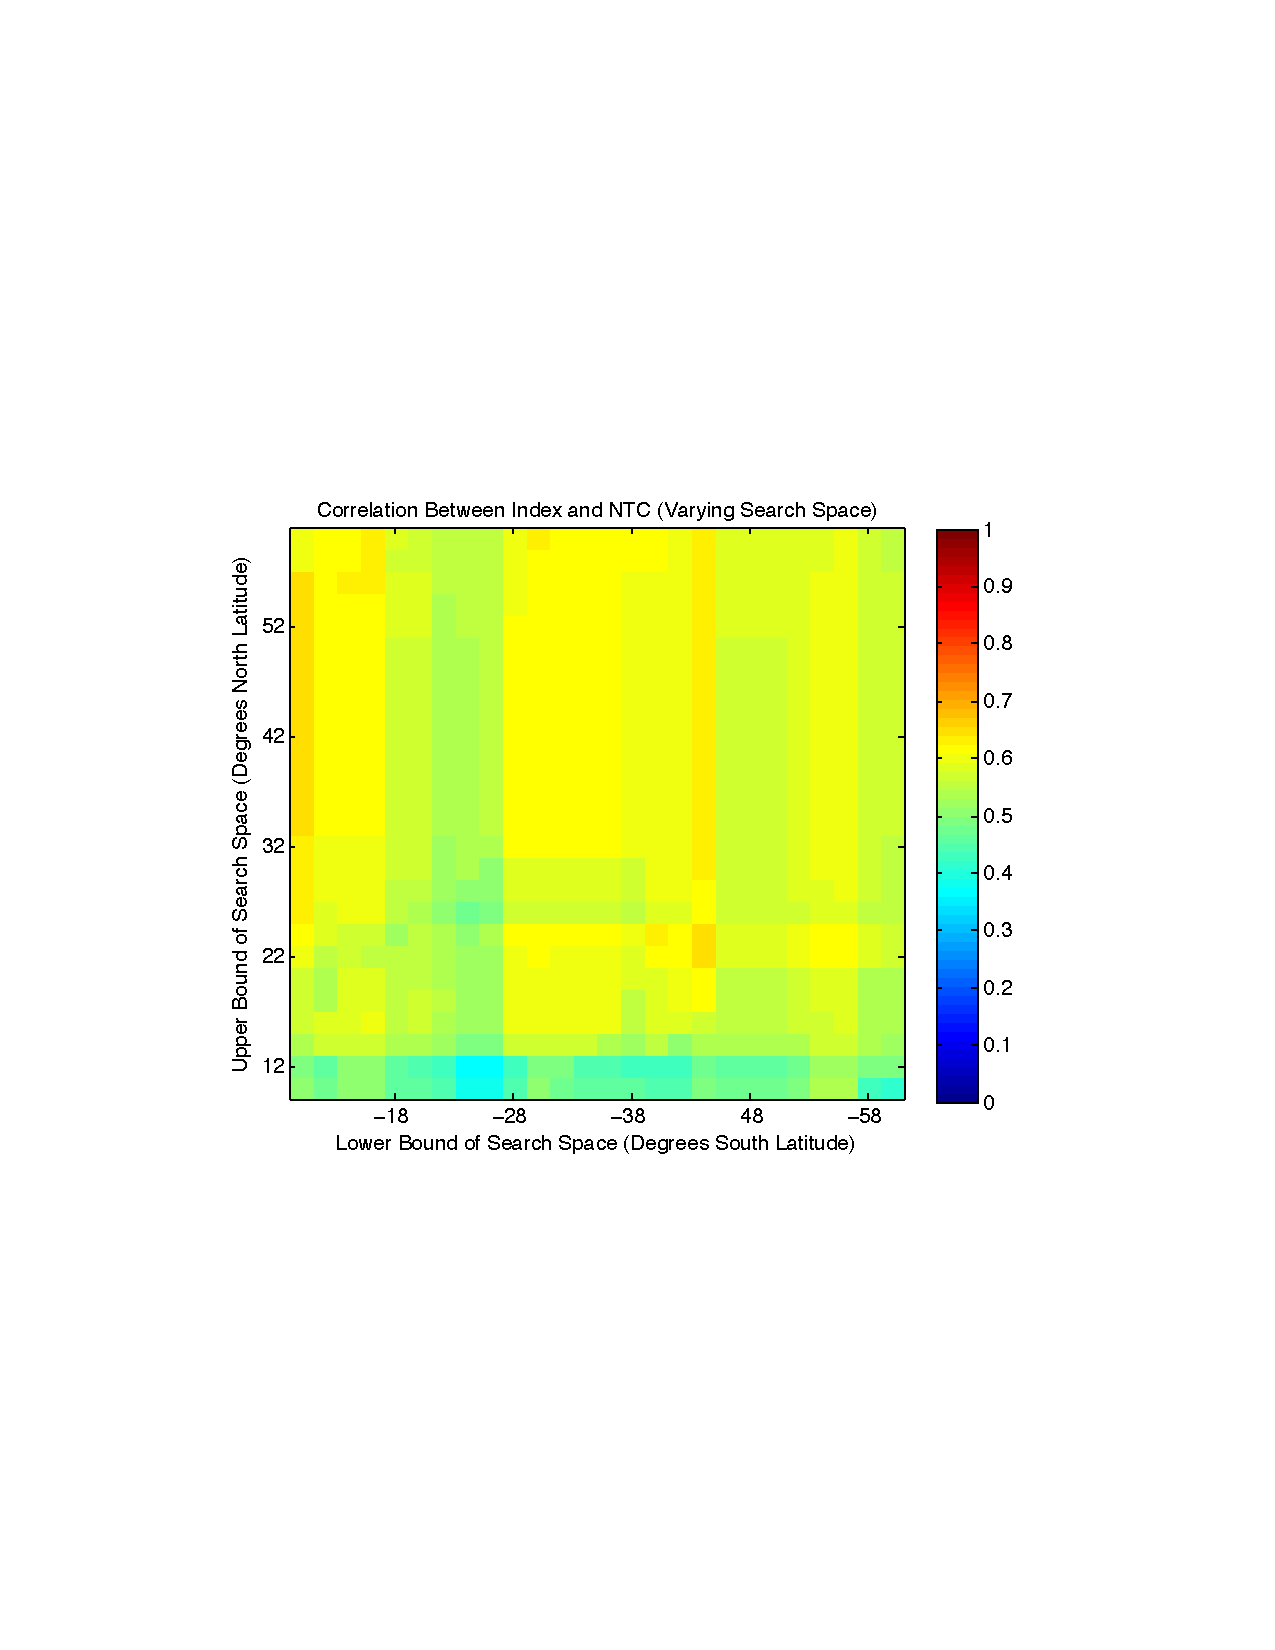
\includegraphics[width=\textwidth]{figures/sensitivityResults/northSouthHem/NTC_Index_North_South.pdf}
\caption{Corr Index vs. NTC}
\label{fig:figure11}
\end{minipage}
\hspace{0cm}
\begin{minipage}[b]{0.6\linewidth}
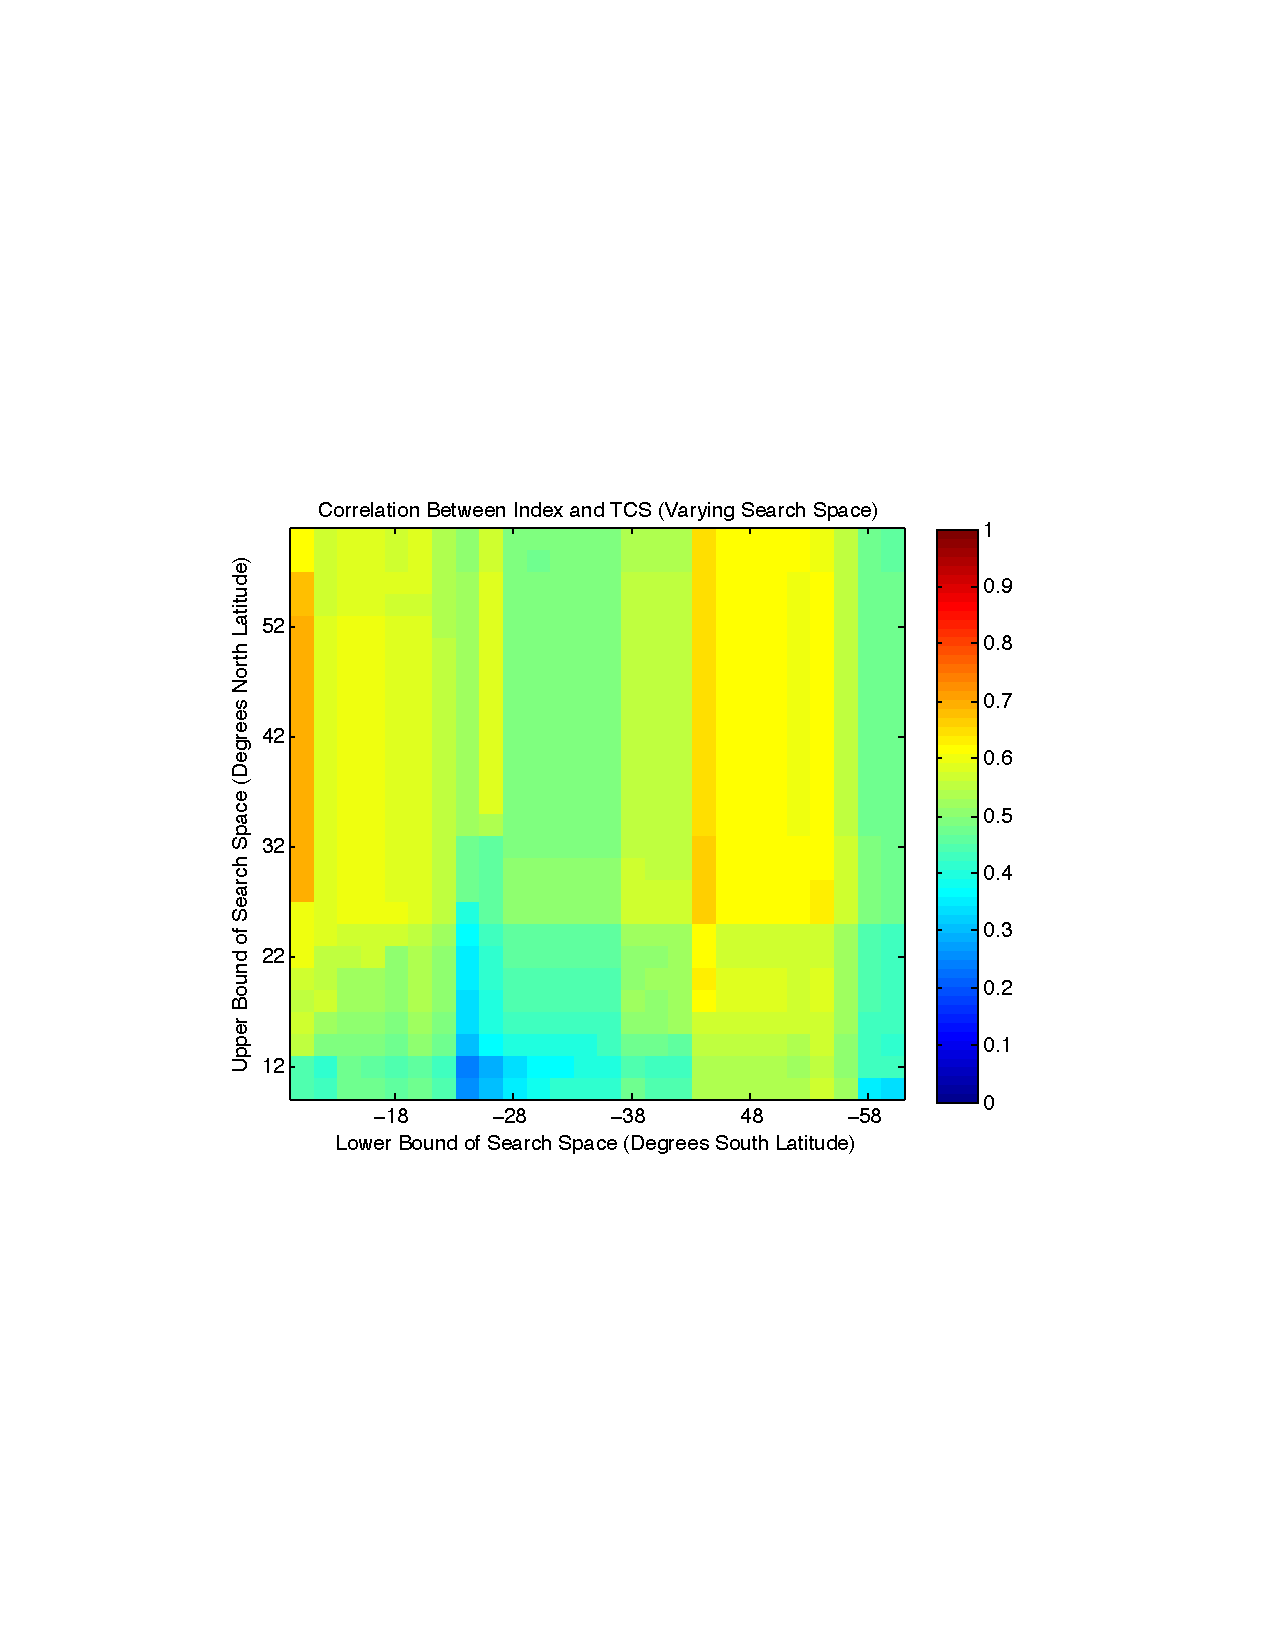
\includegraphics[width=\textwidth]{figures/sensitivityResults/northSouthHem/TCS_Index_North_South.pdf}
\caption{Corr Index vs. TCs}
\label{fig:figure12}
\end{minipage}
\end{figure}
\pagebreak

\subsection{Varying Search Space (North Hemisphere)}

\begin{figure}[ht]
\begin{minipage}[b]{0.6\linewidth}
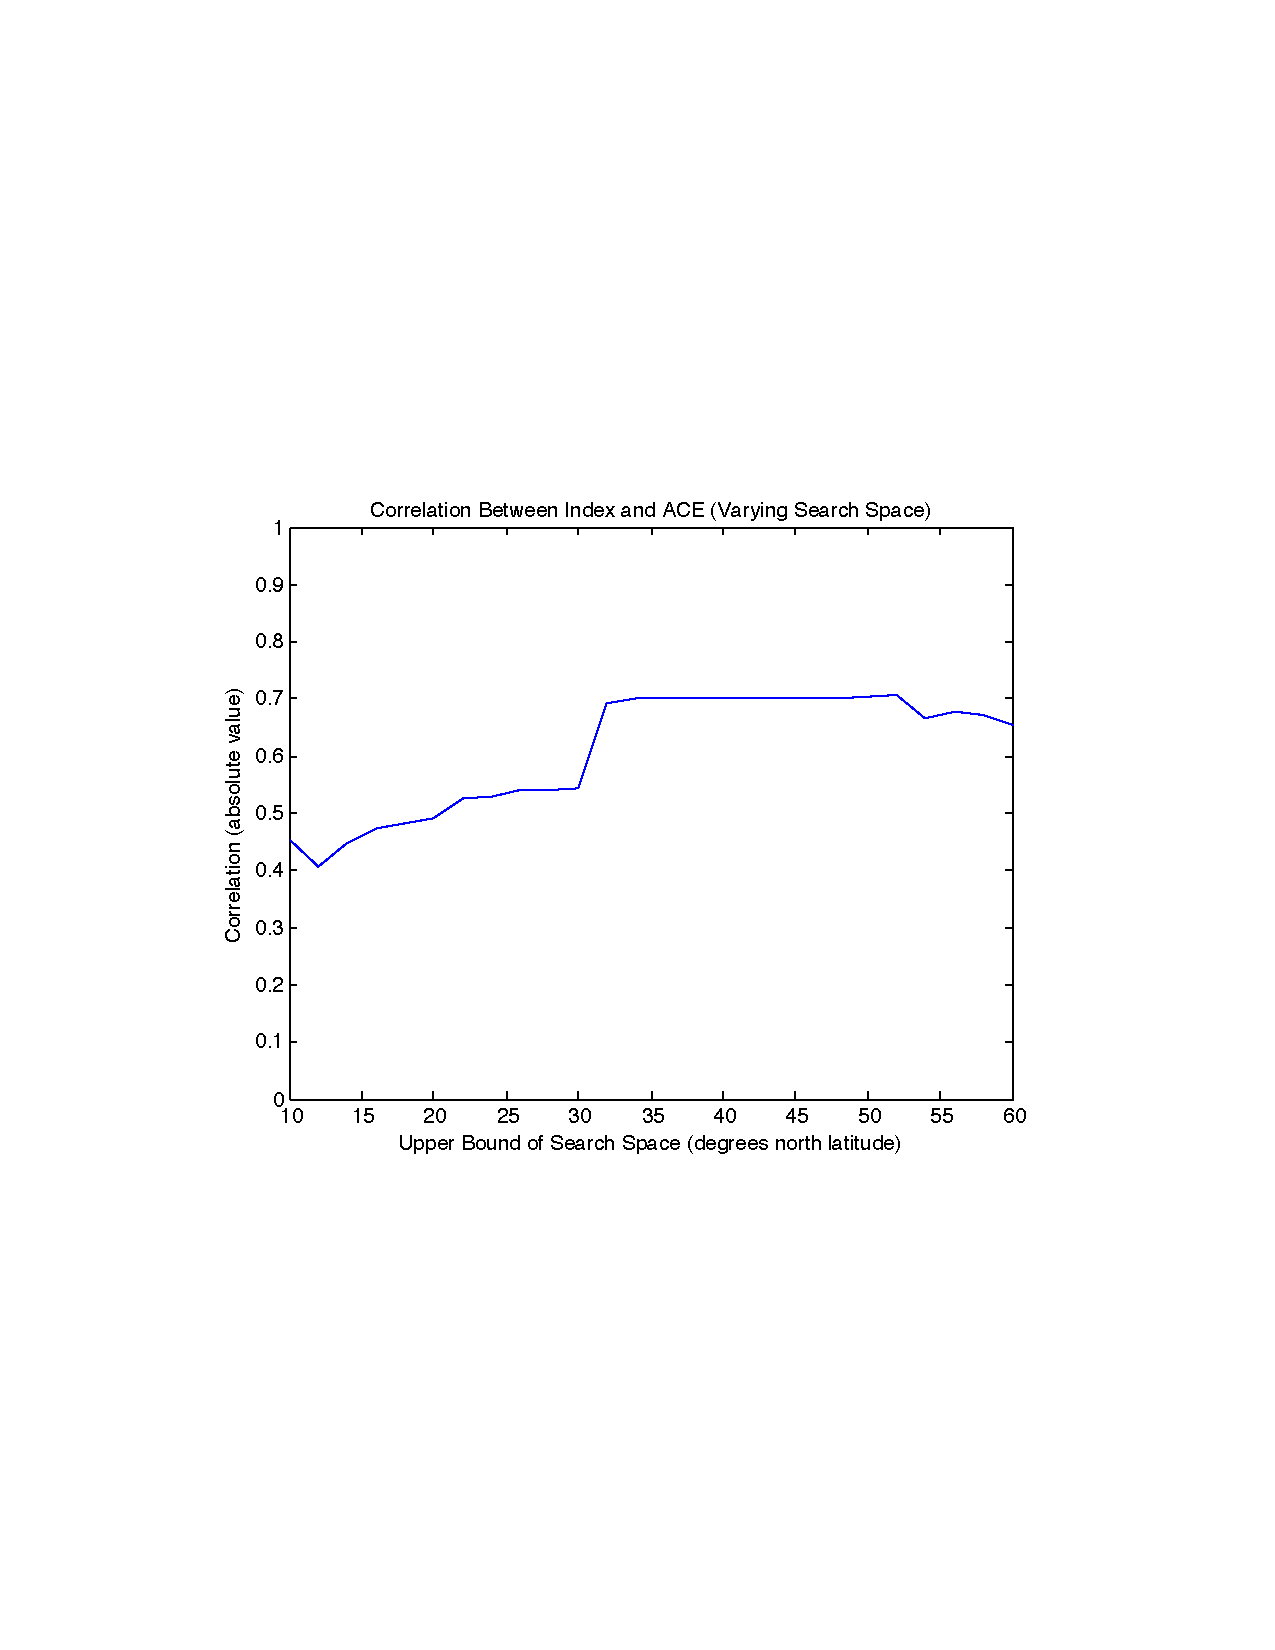
\includegraphics[width=\textwidth]{figures/sensitivityResults/northHem/ACE_Index_North.pdf}
\caption{Corr Index vs. ACE}
\label{fig:figure13}
\end{minipage}
\hspace{0cm}
\begin{minipage}[b]{0.6\linewidth}
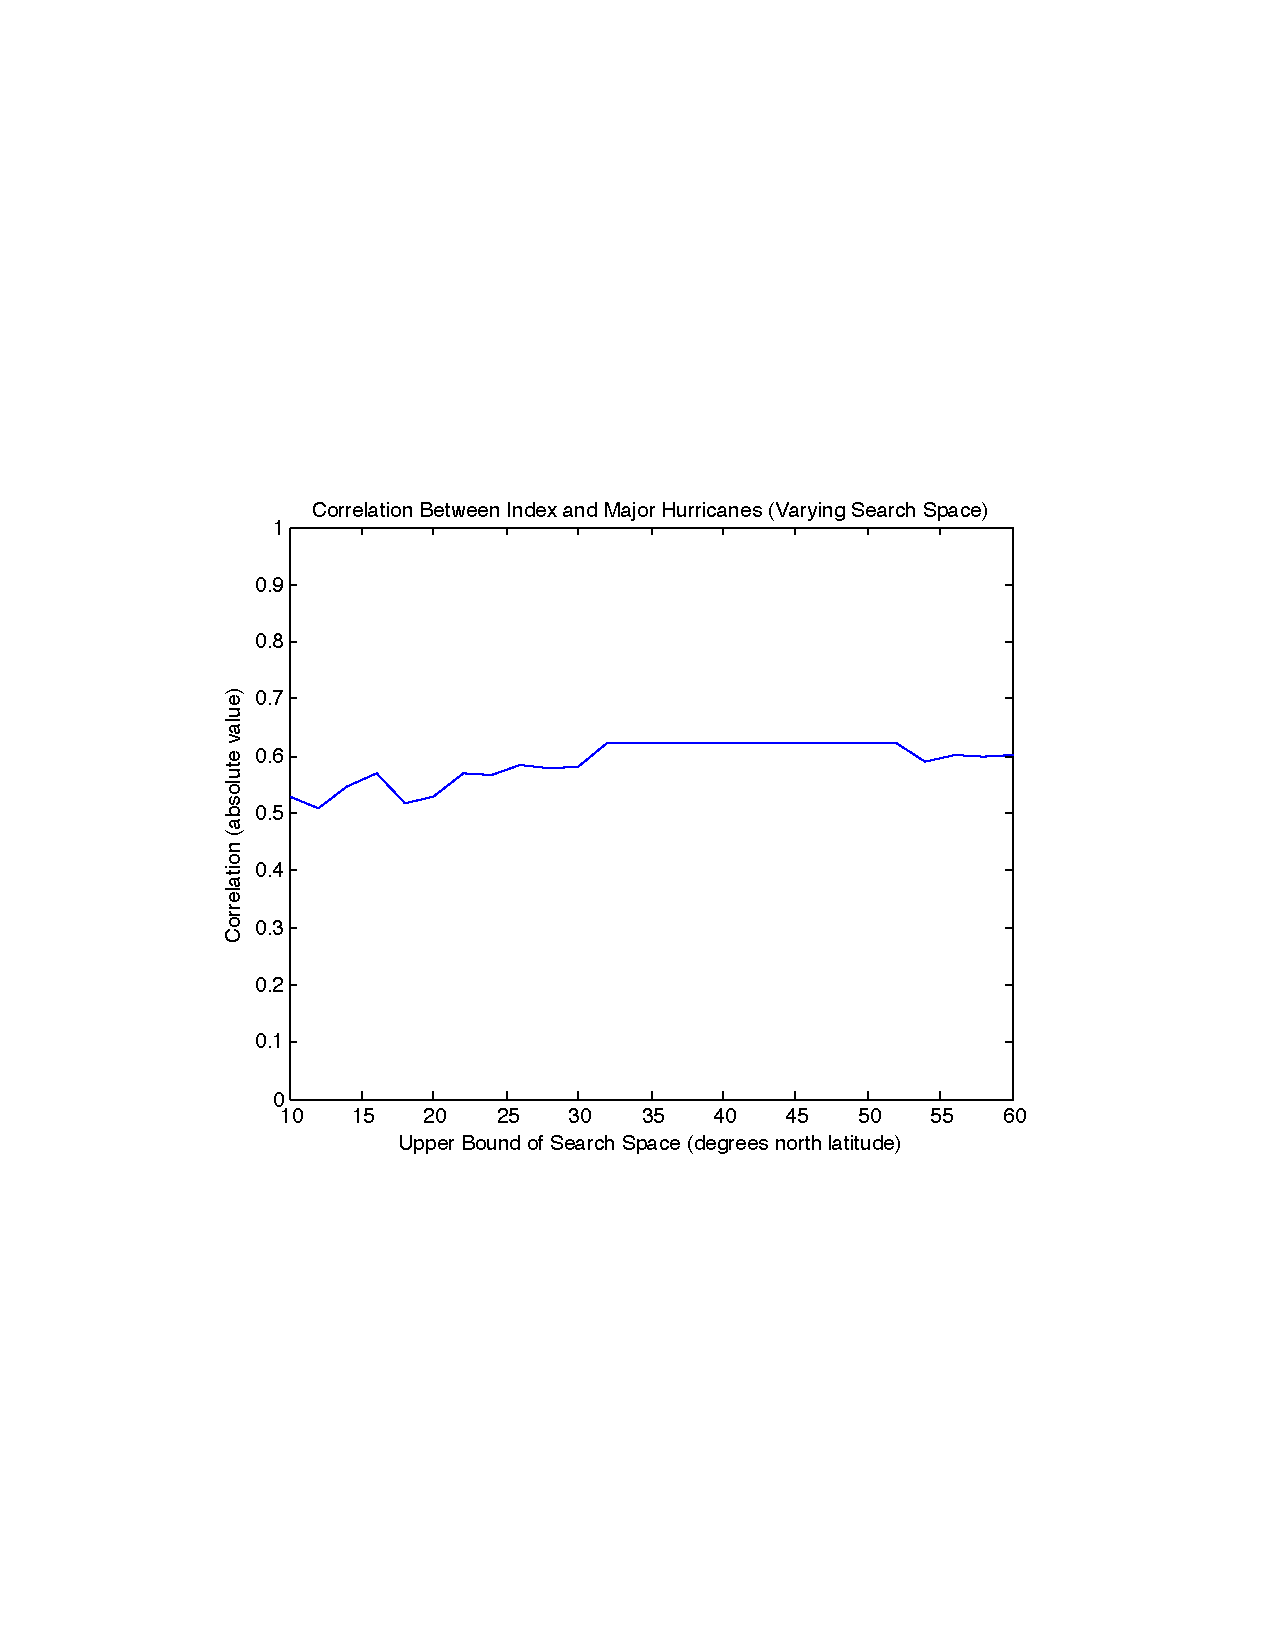
\includegraphics[width=\textwidth]{figures/sensitivityResults/northHem/Major_Hurricanes_Index_North.pdf}
\caption{Corr Index vs. Major Hurricanes}
\label{fig:figure14}
\end{minipage}
\end{figure}

\begin{figure}[ht]
\begin{minipage}[b]{0.6\linewidth}
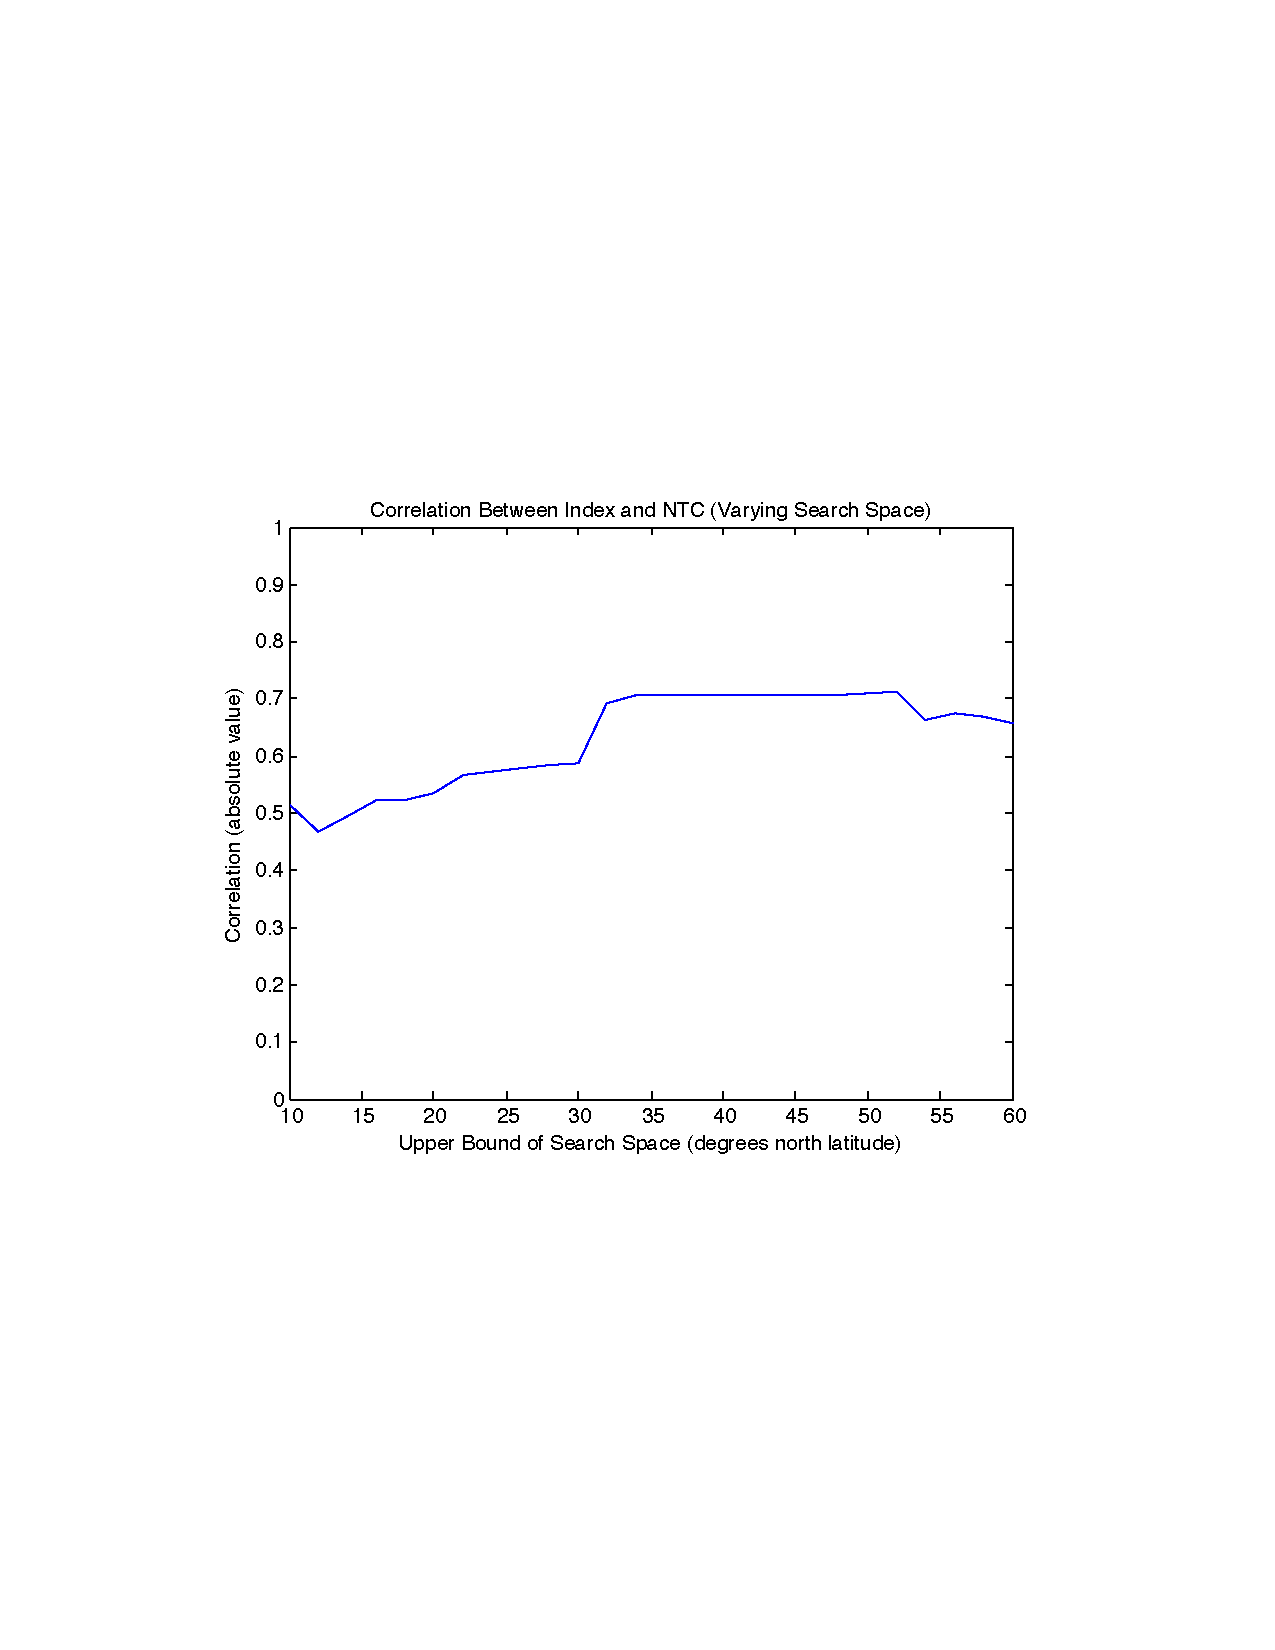
\includegraphics[width=\textwidth]{figures/sensitivityResults/northHem/NTC_Index_North.pdf}
\caption{Corr Index vs. NTC}
\label{fig:figure15}
\end{minipage}
\hspace{0cm}
\begin{minipage}[b]{0.6\linewidth}
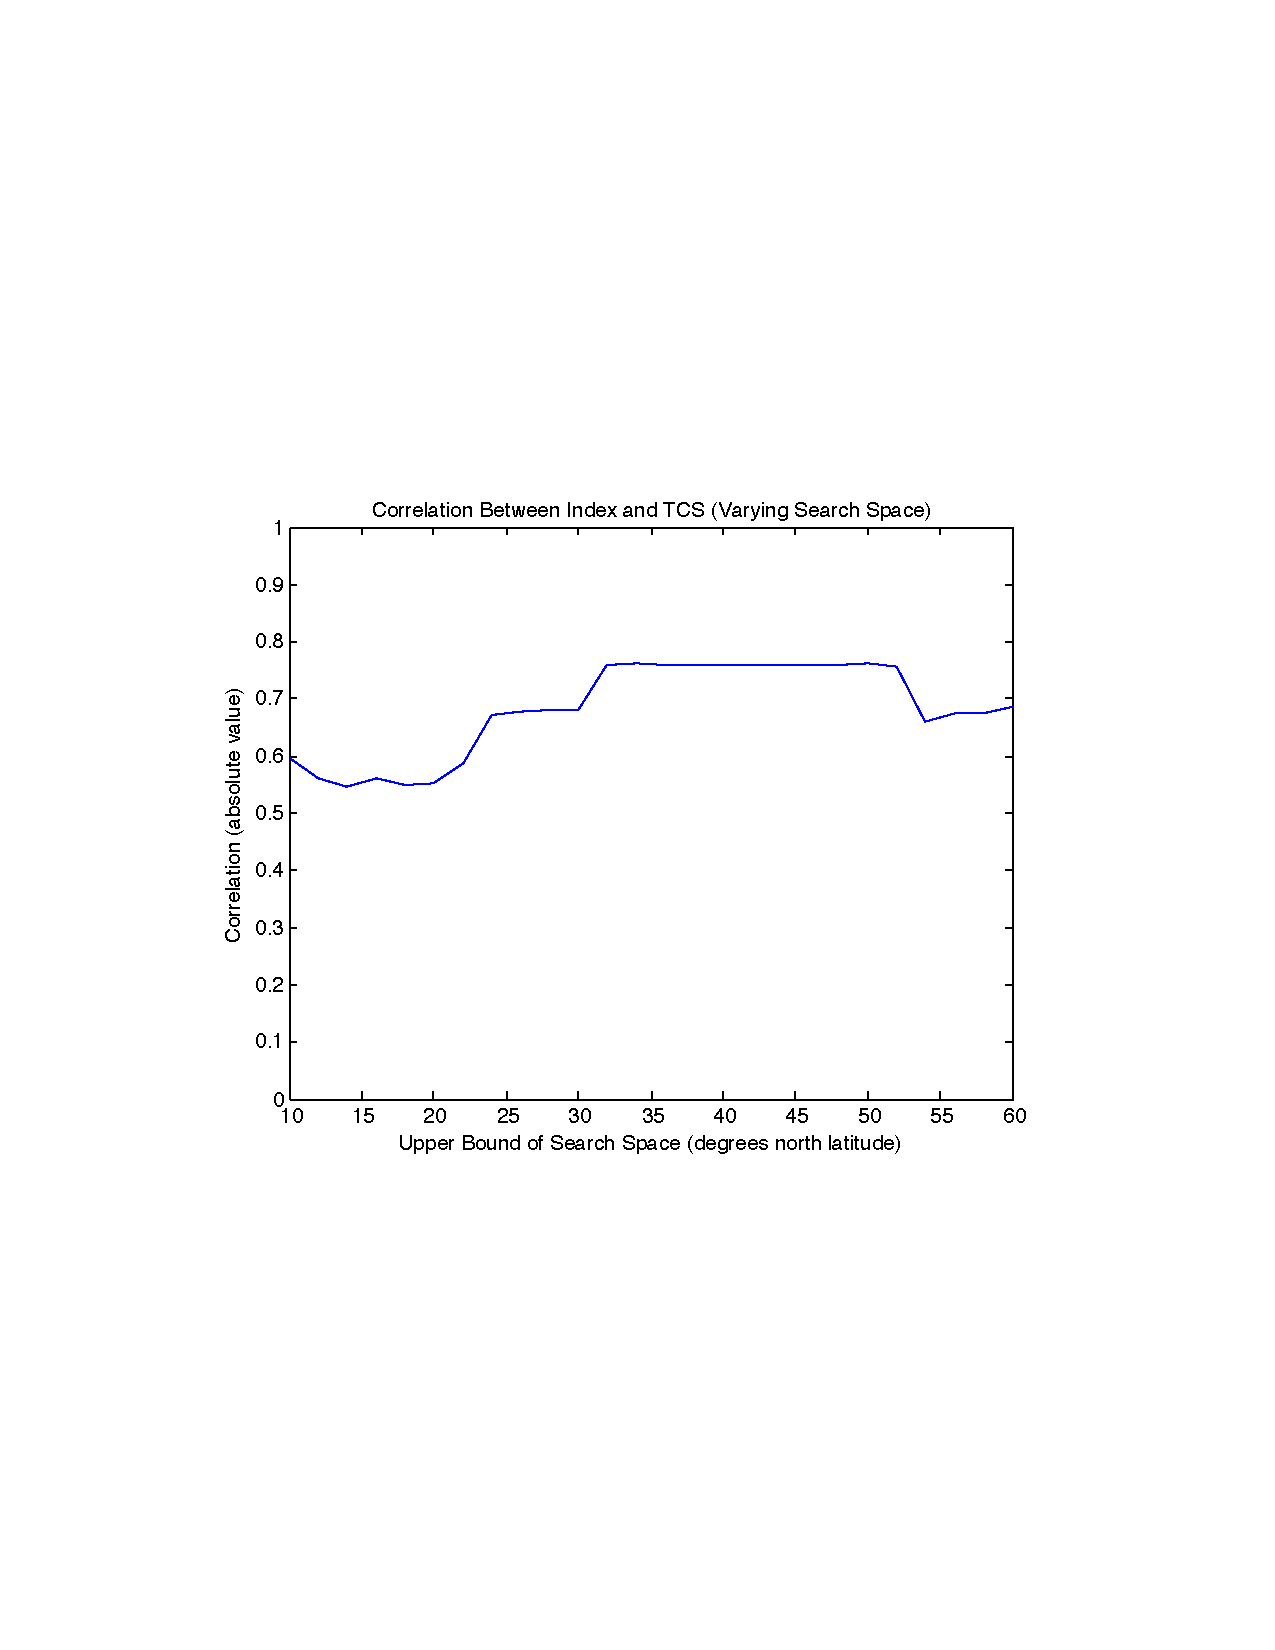
\includegraphics[width=\textwidth]{figures/sensitivityResults/northHem/TCS_Index_North.pdf}
\caption{Corr Index vs. TCs}
\label{fig:figure16}
\end{minipage}
\end{figure}
\pagebreak
\subsection{Varying Hurricane Season}

\begin{figure}[ht]
\begin{minipage}[b]{0.6\linewidth}
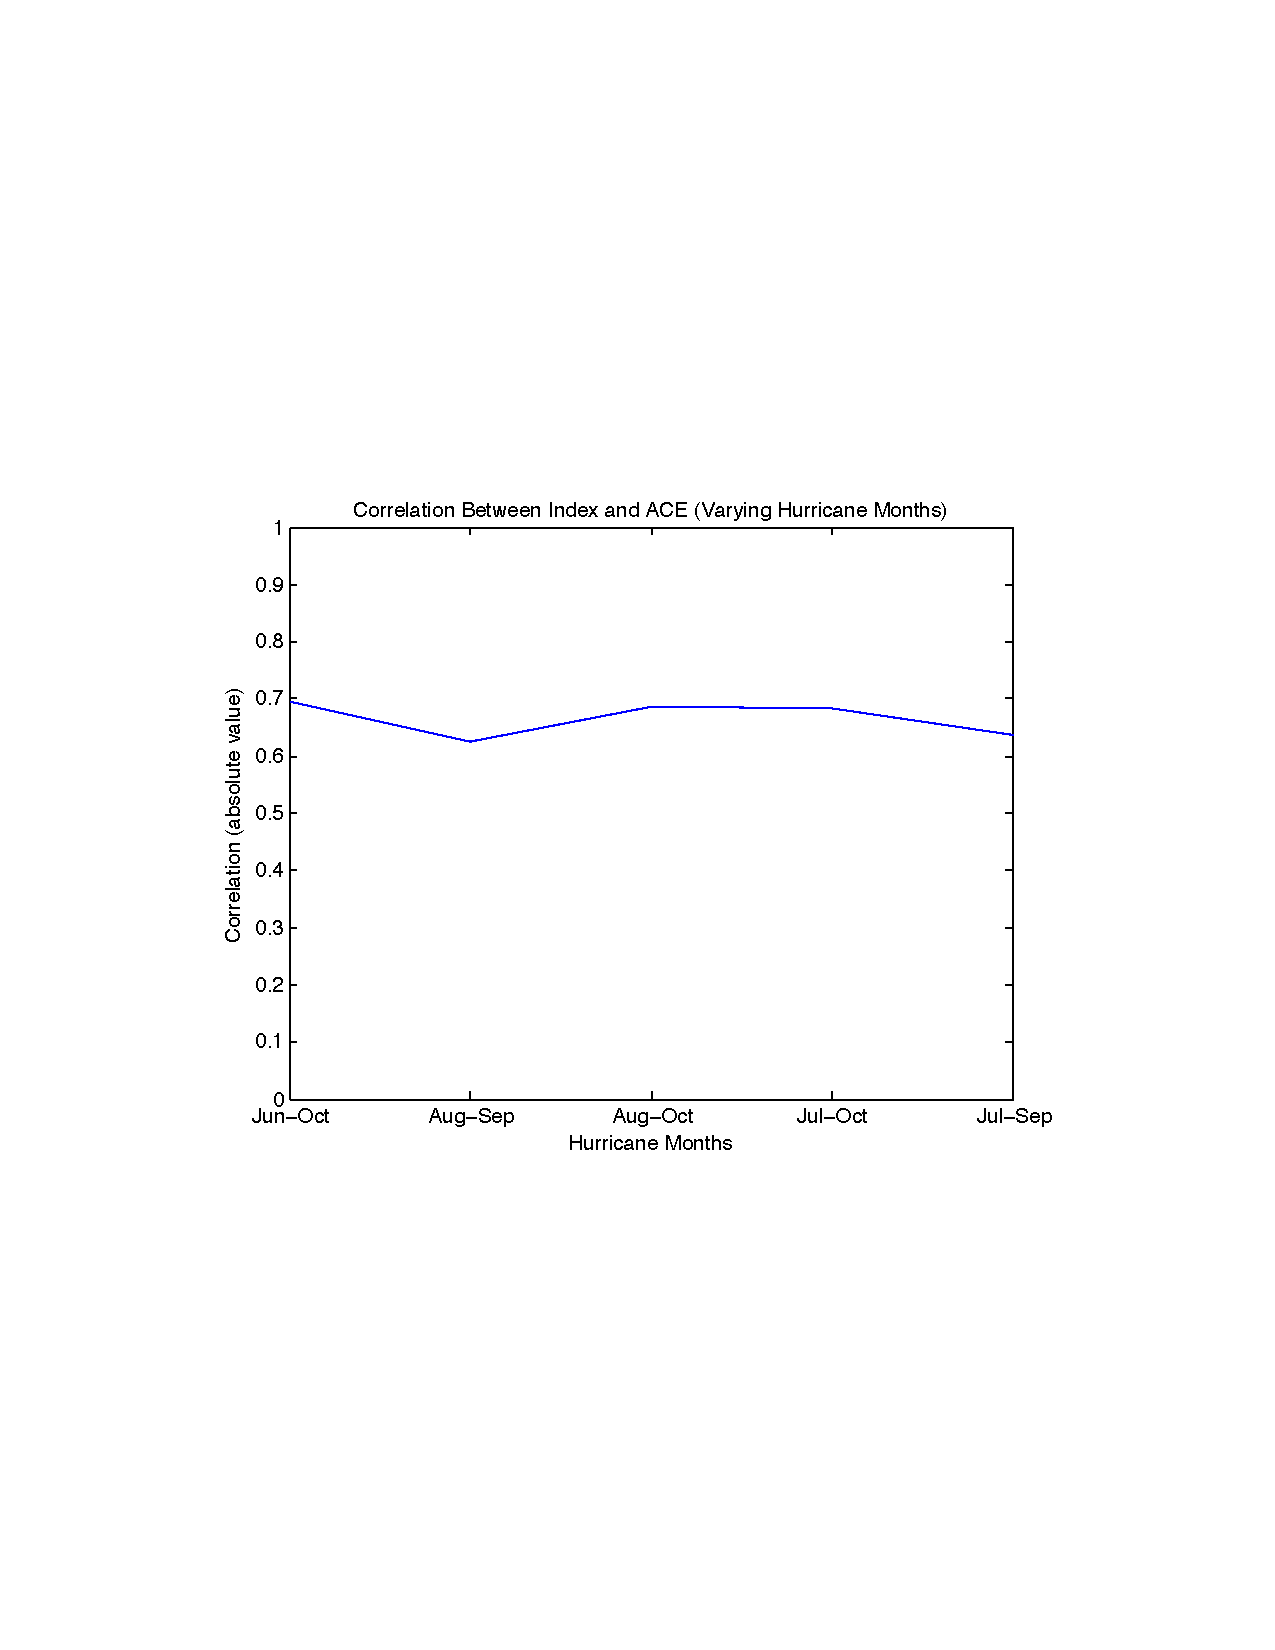
\includegraphics[width=\textwidth]{figures/sensitivityResults/hurrMonths/ACE_Index_Hurr_Months.pdf}
\caption{Corr Index vs. ACE}
\label{fig:figure17}
\end{minipage}
\hspace{0cm}
\begin{minipage}[b]{0.6\linewidth}
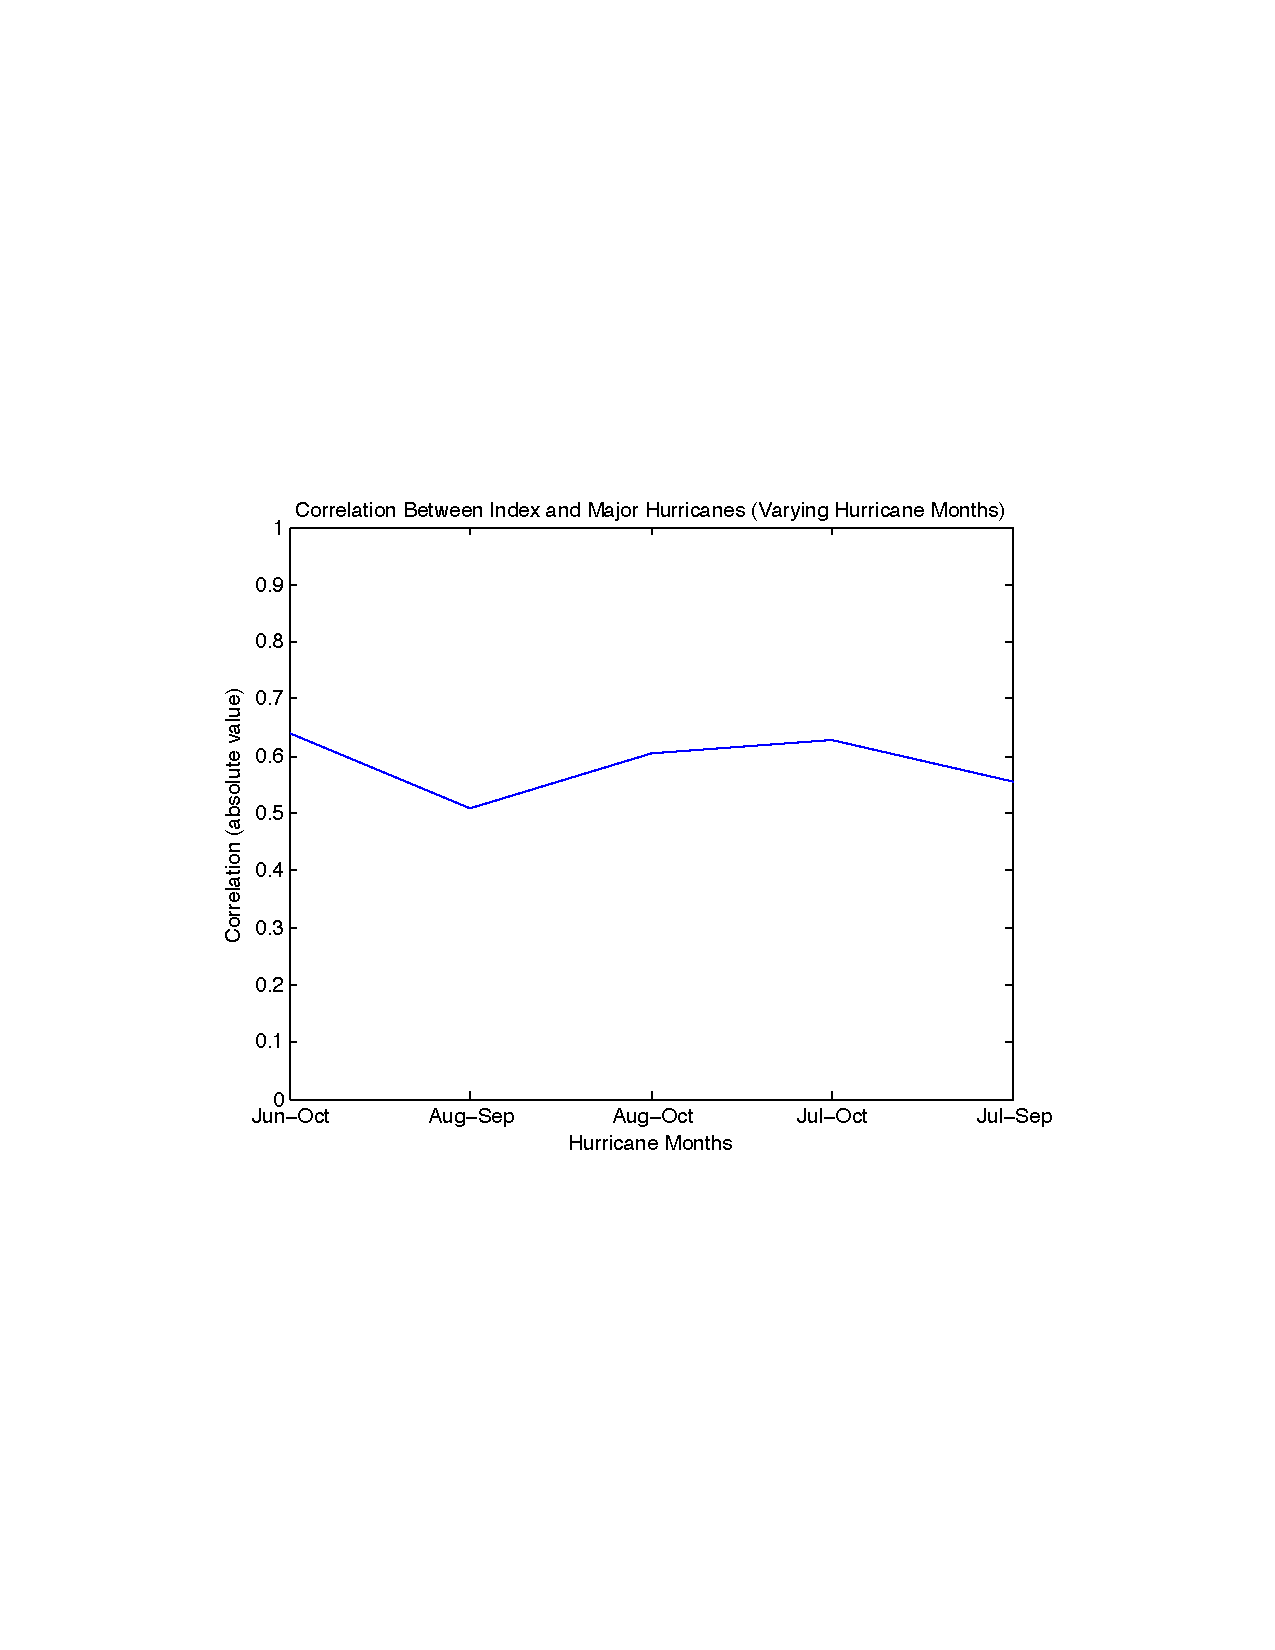
\includegraphics[width=\textwidth]{figures/sensitivityResults/hurrMonths/Major_Hurricanes_Index_Hurr_Months.pdf}
\caption{Corr Index vs. Major Hurricanes}
\label{fig:figure18}
\end{minipage}
\end{figure}
\begin{figure}[ht]
\begin{minipage}[b]{0.6\linewidth}
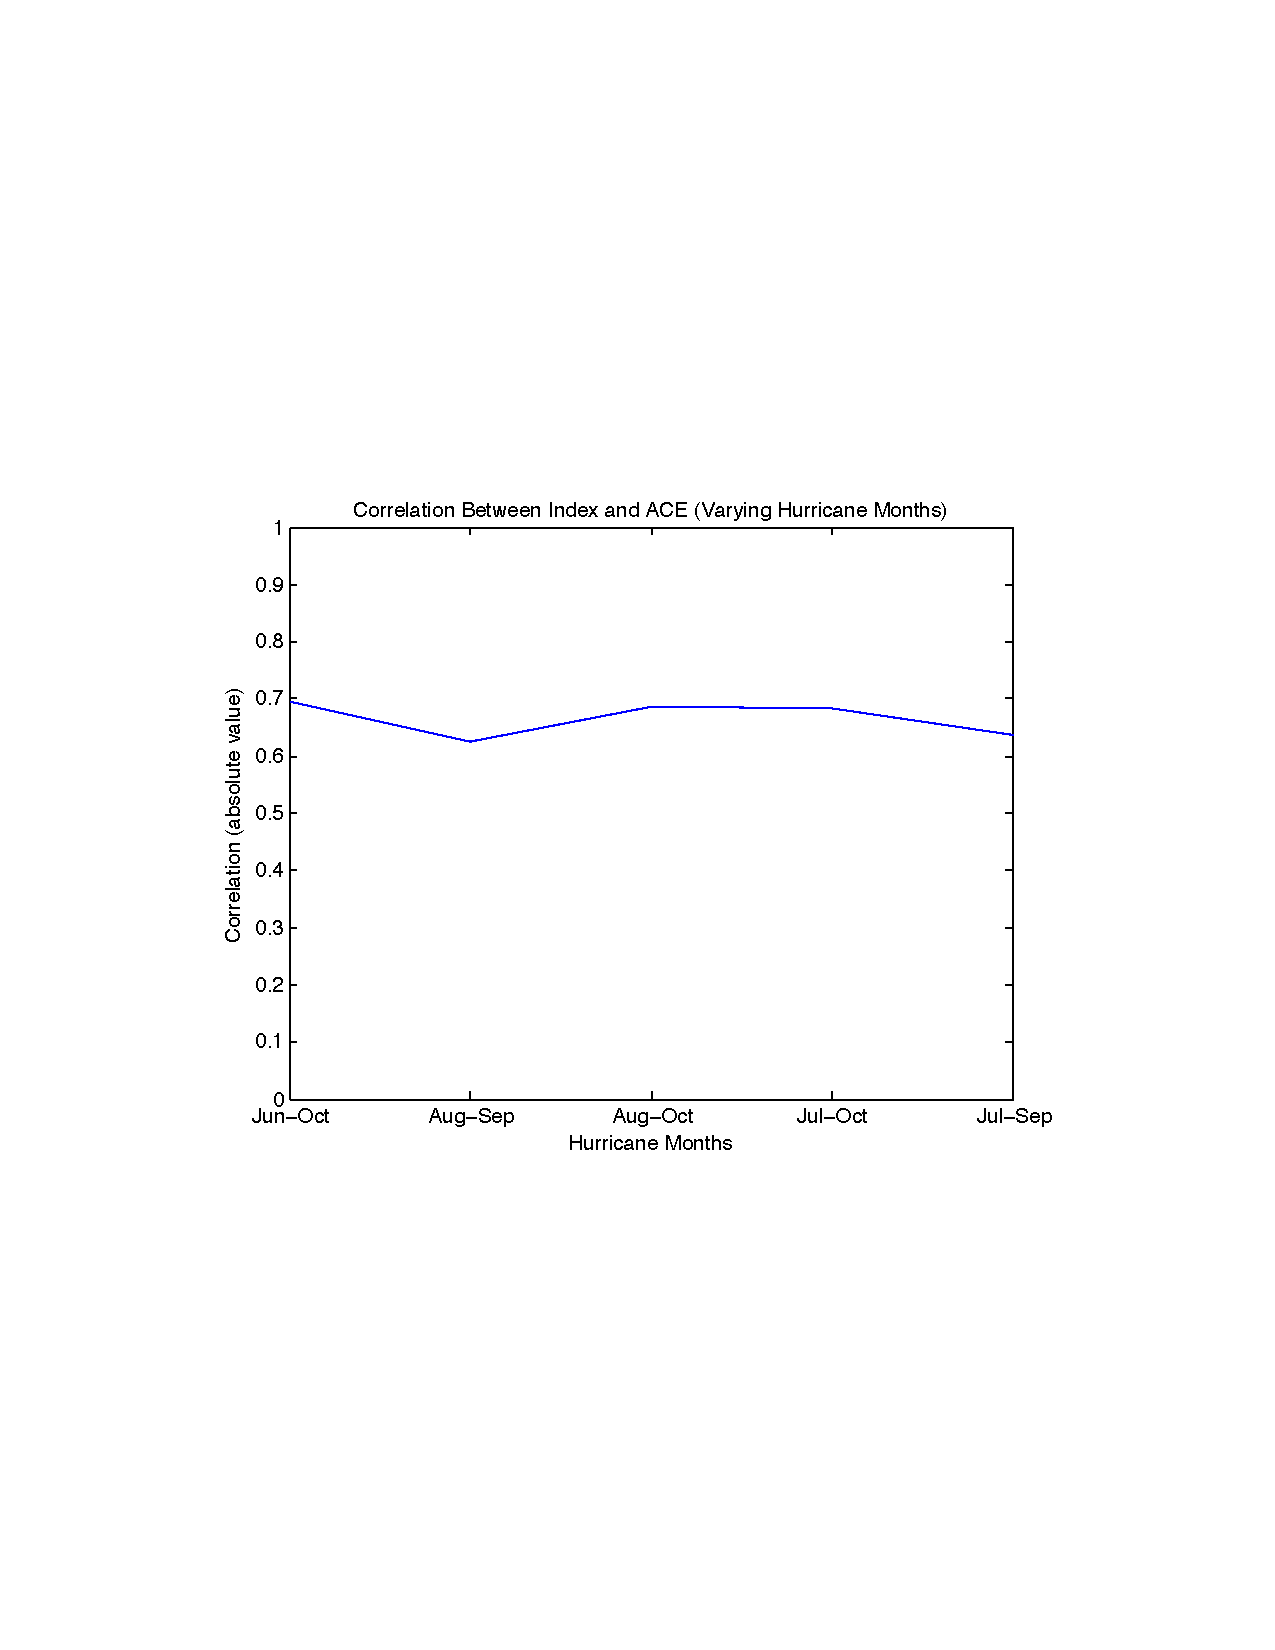
\includegraphics[width=\textwidth]{figures/sensitivityResults/hurrMonths/ACE_Index_Hurr_Months.pdf}
\caption{Corr Index vs. ACE}
\label{fig:figure19}
\end{minipage}
\hspace{0cm}
\begin{minipage}[b]{0.6\linewidth}
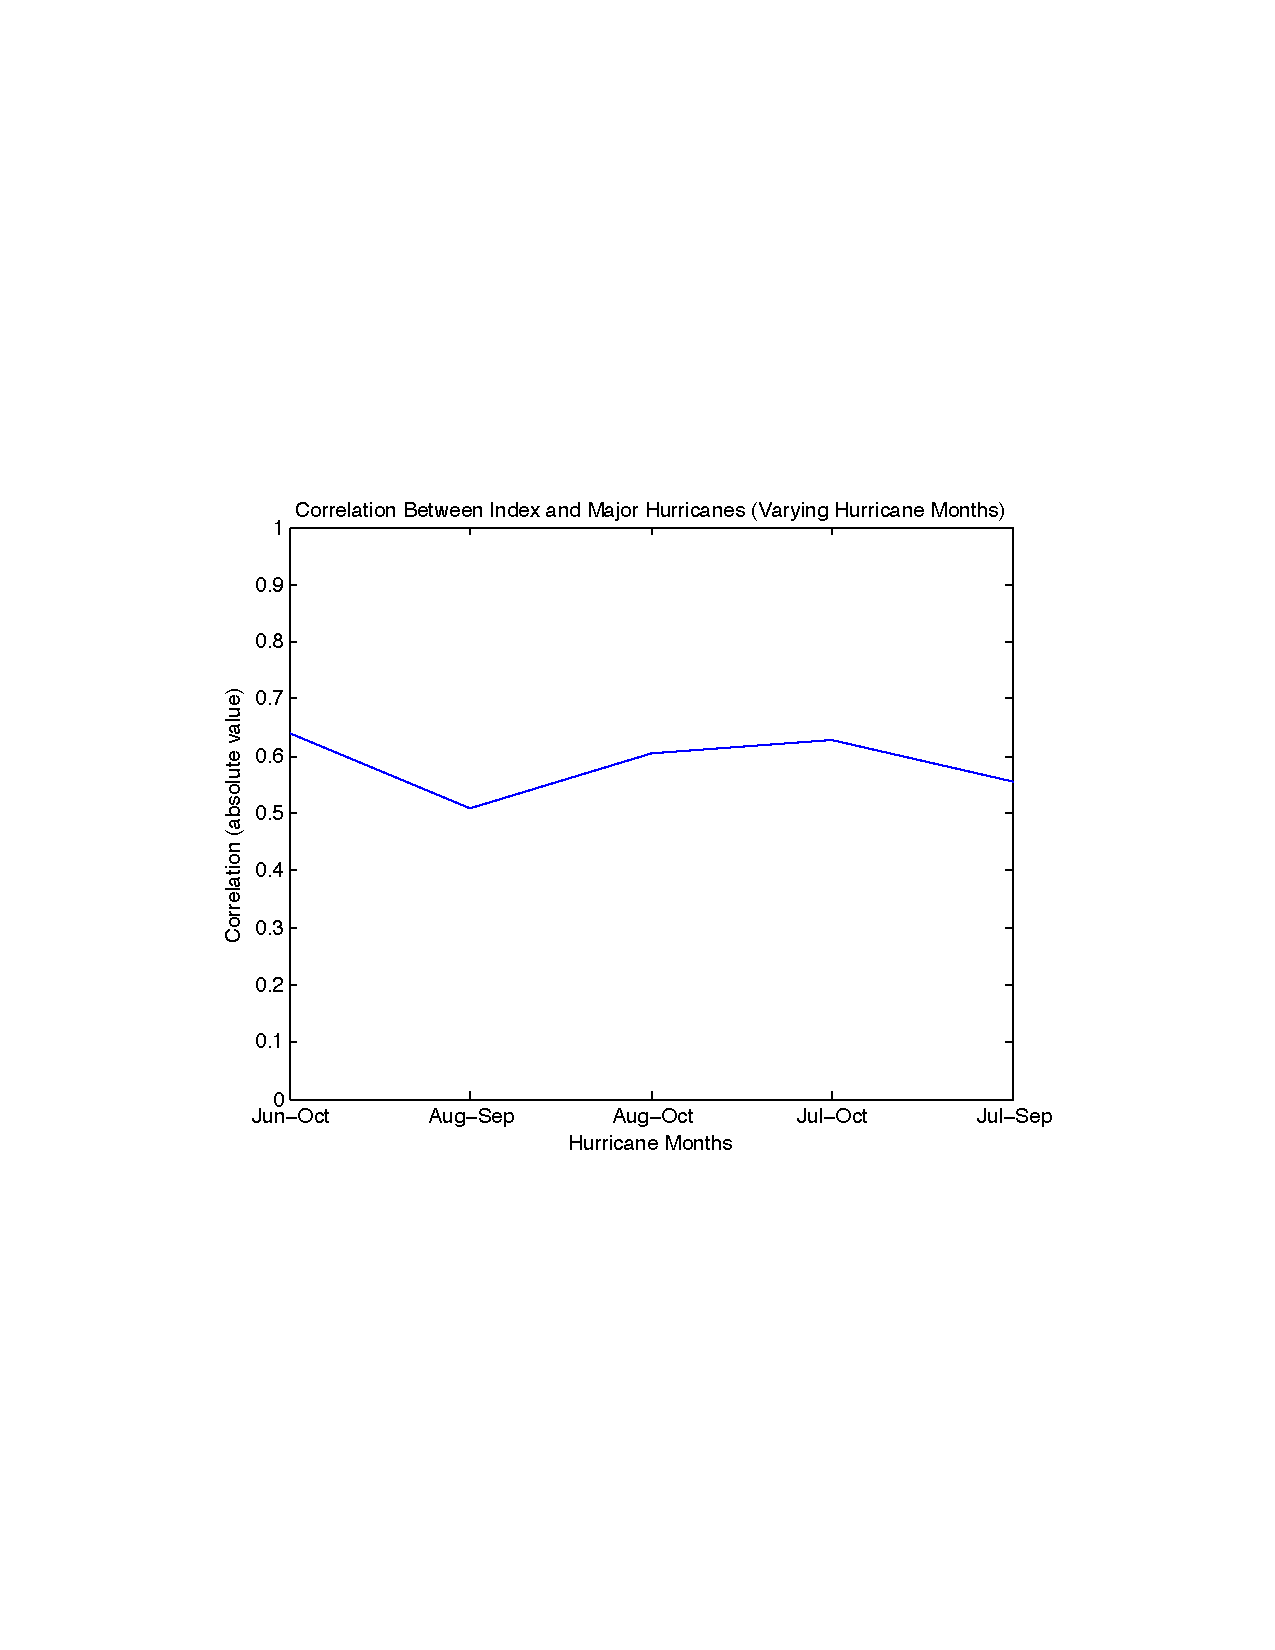
\includegraphics[width=\textwidth]{figures/sensitivityResults/hurrMonths/Major_Hurricanes_Index_Hurr_Months.pdf}
\caption{Corr Index vs. Major Hurricanes}
\label{fig:figure20}
\end{minipage}
\end{figure}

\pagebreak
\section{Difference Composite Maps}
\begin{figure}[ht]
\begin{minipage}[b]{0.55\linewidth}
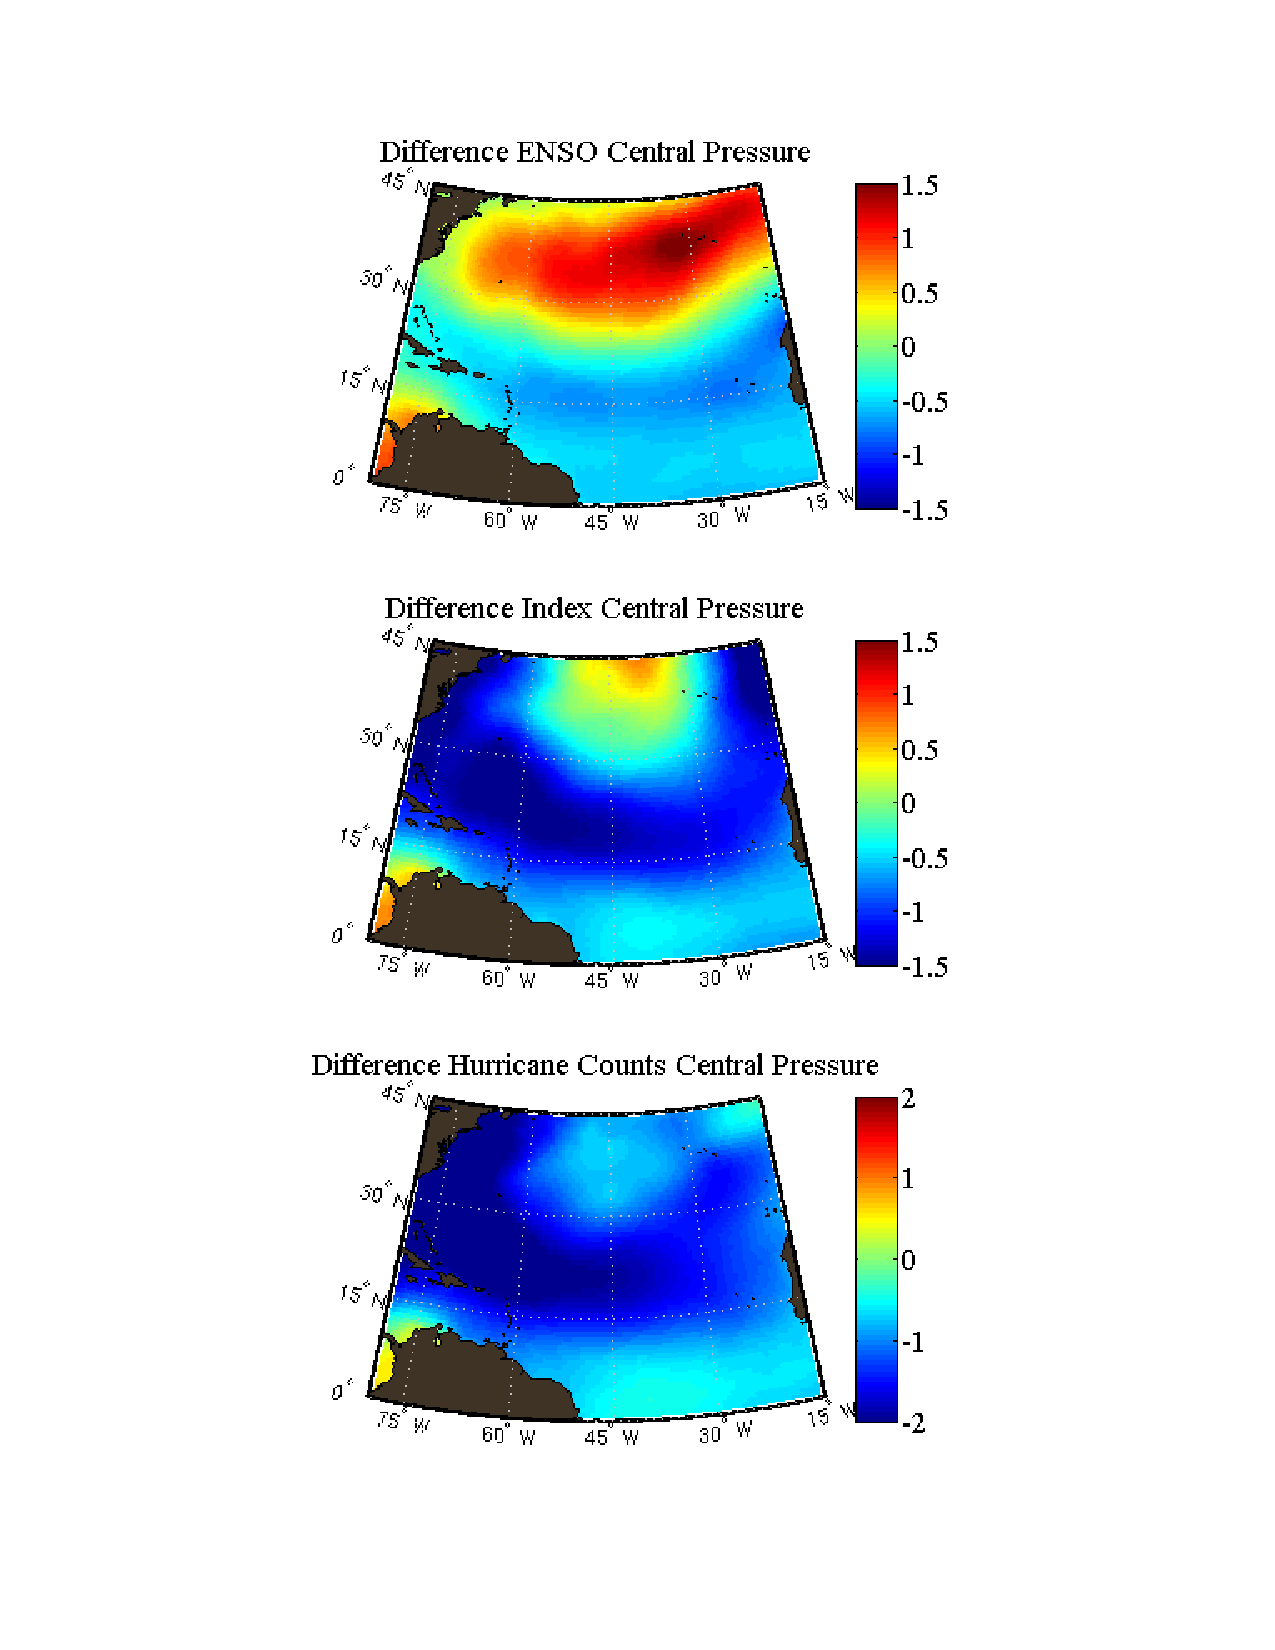
\includegraphics[width=\textwidth]{figures/sensitivityResults/compositeMaps/centralPressureAtlanticMap.pdf}
\caption{Diff Pressure Composites}
\label{fig:figure21}
\end{minipage}
\hspace{0cm}
\begin{minipage}[b]{0.55\linewidth}
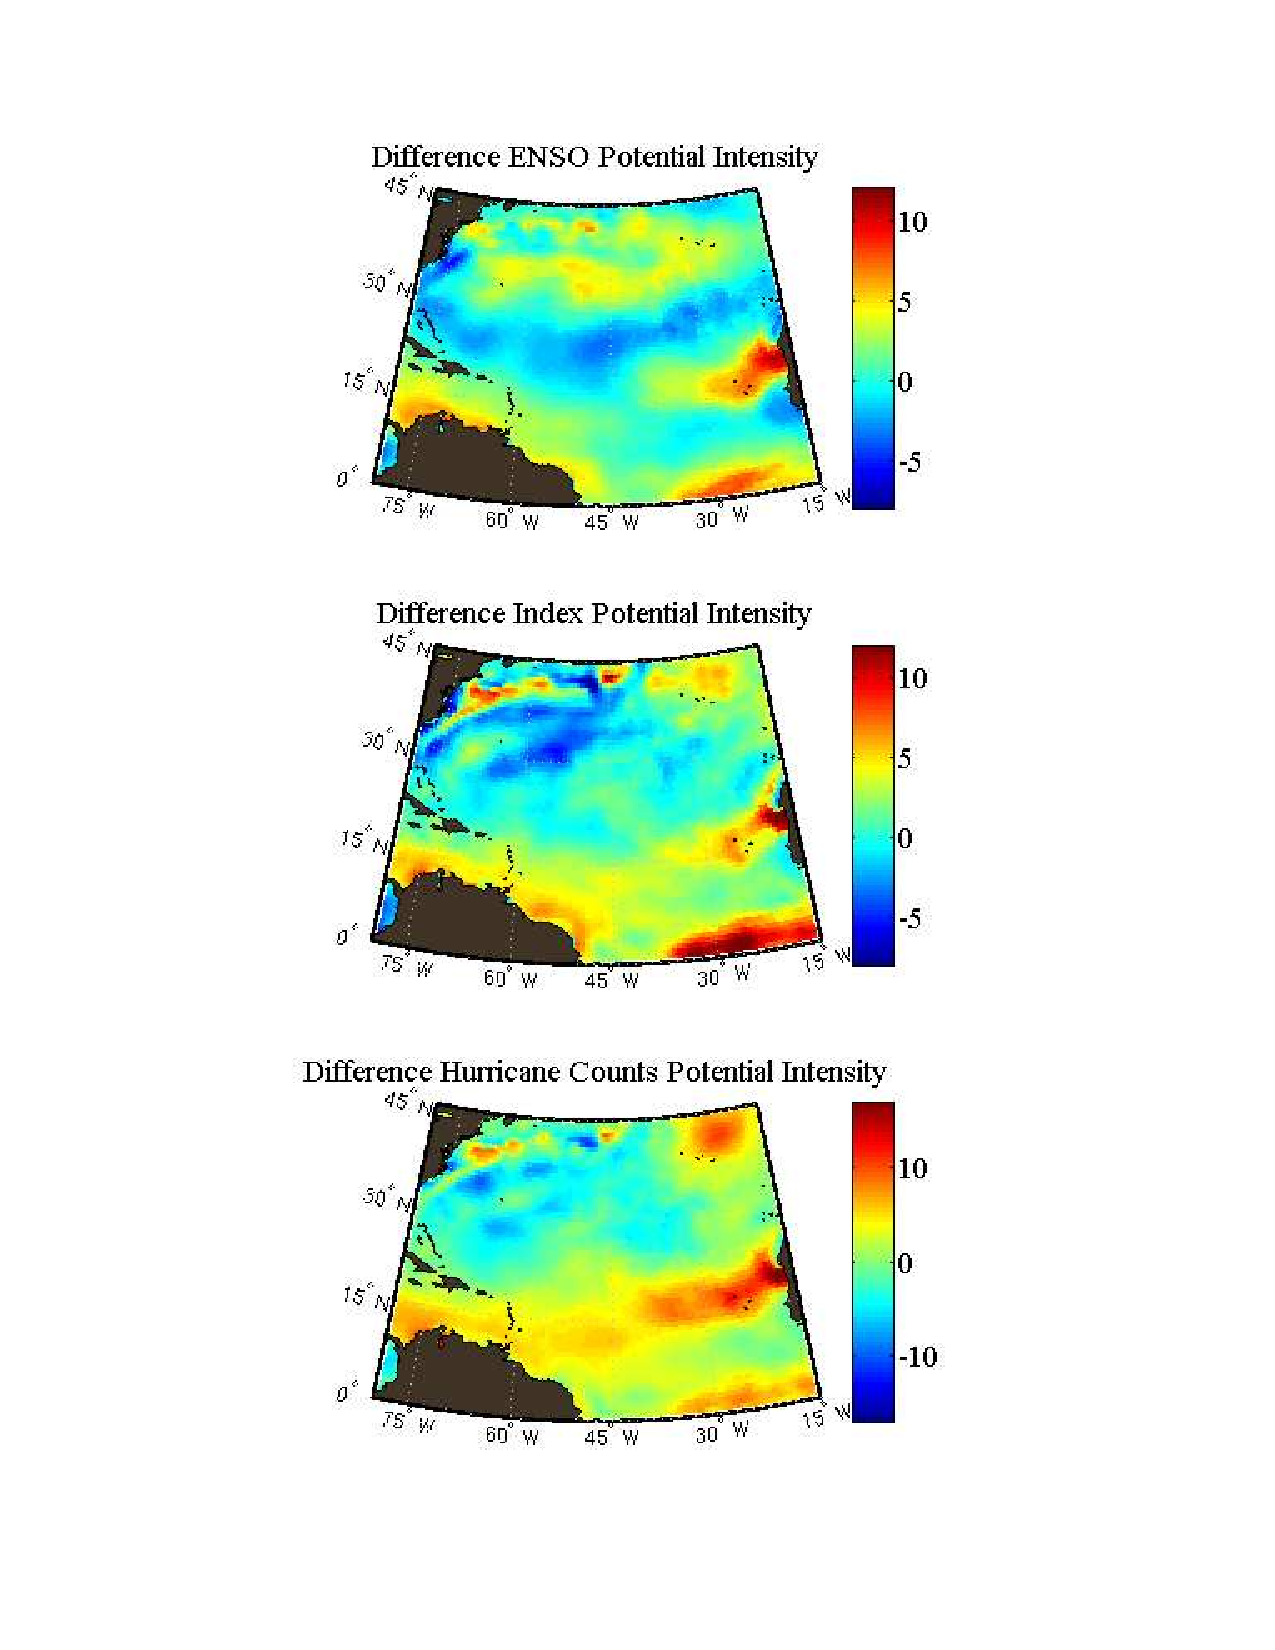
\includegraphics[width=\textwidth]{figures/sensitivityResults/compositeMaps/diffPIAtlanticComposites.pdf}
\caption{Diff PI Composites}
\label{fig:figure22}
\end{minipage}
\end{figure}

\pagebreak
\begin{figure}[ht]
\begin{minipage}[b]{0.6\linewidth}
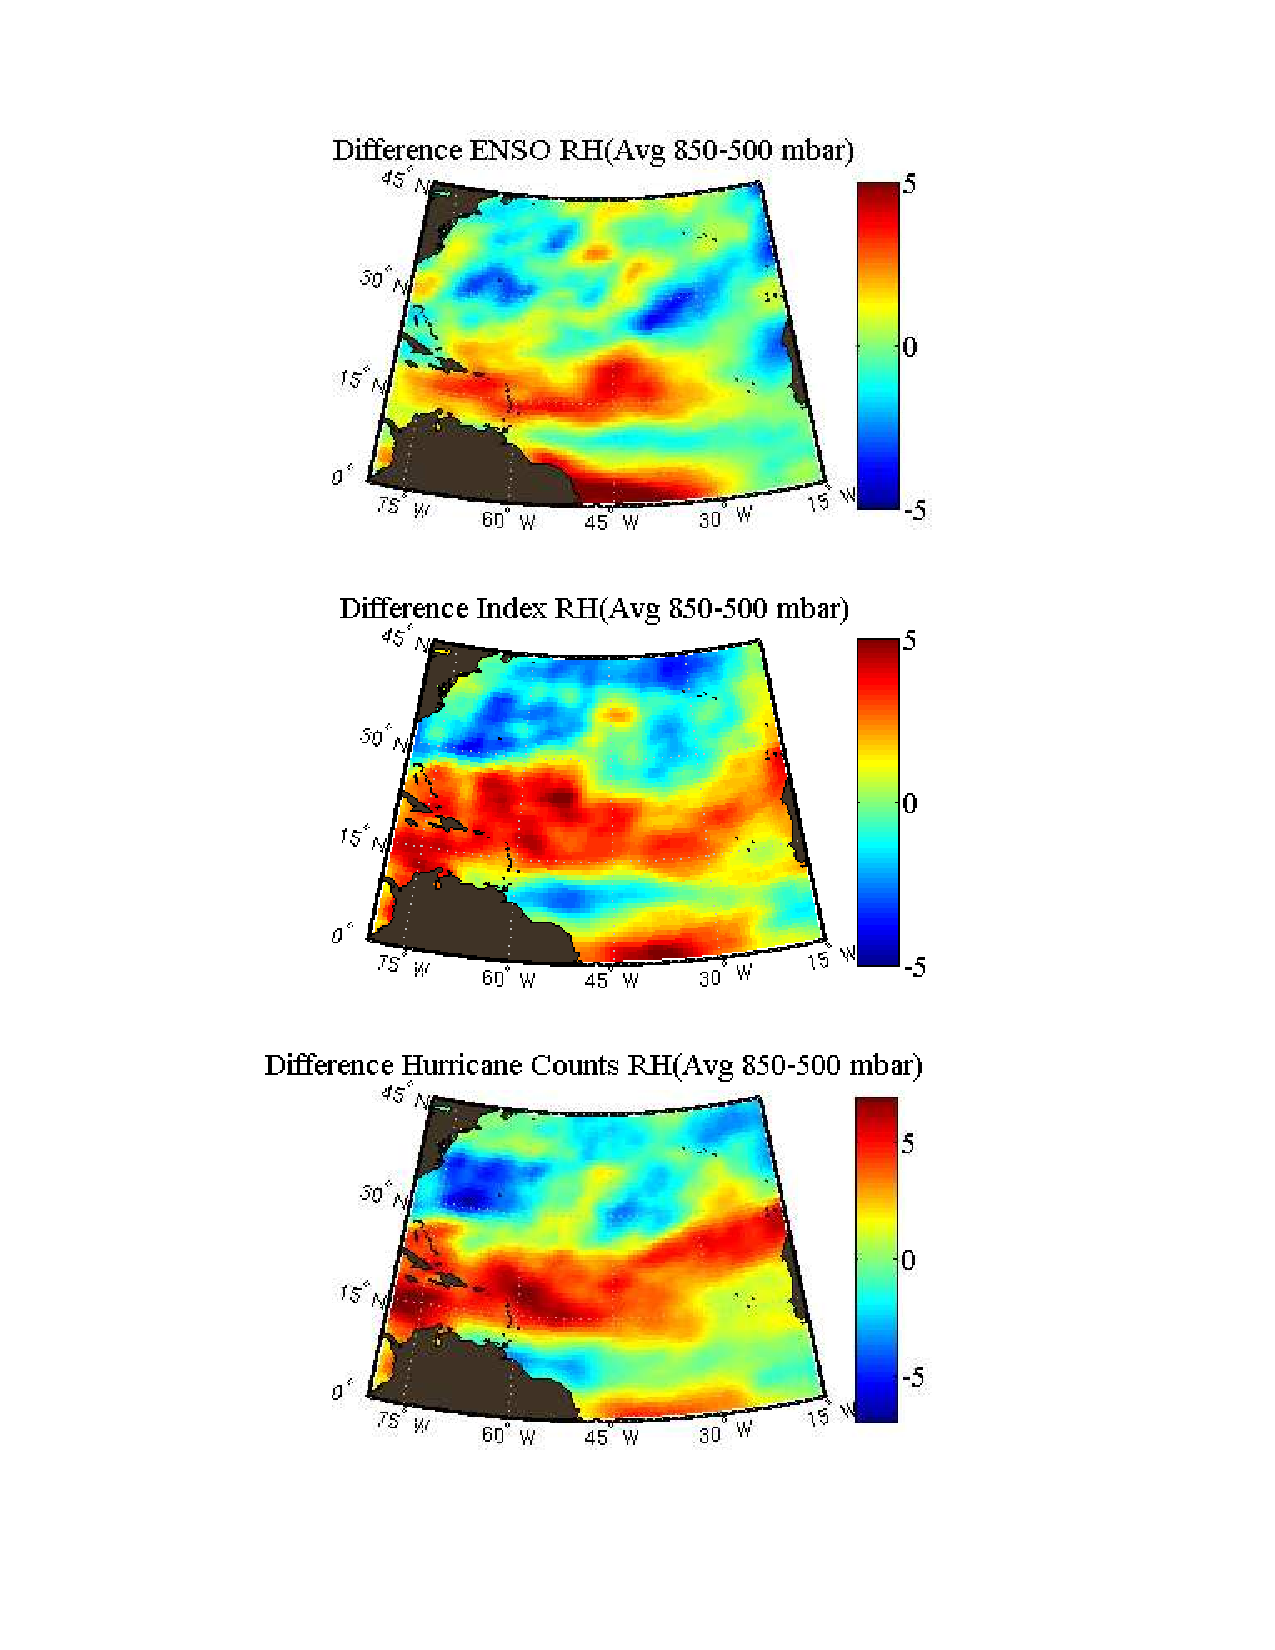
\includegraphics[width=\textwidth]{figures/sensitivityResults/compositeMaps/diffRHCompositesAtlanticMap.pdf}
\caption{Diff Relative Humidity}
\label{fig:figure23}
\end{minipage}
\hspace{0cm}
\begin{minipage}[b]{0.6\linewidth}
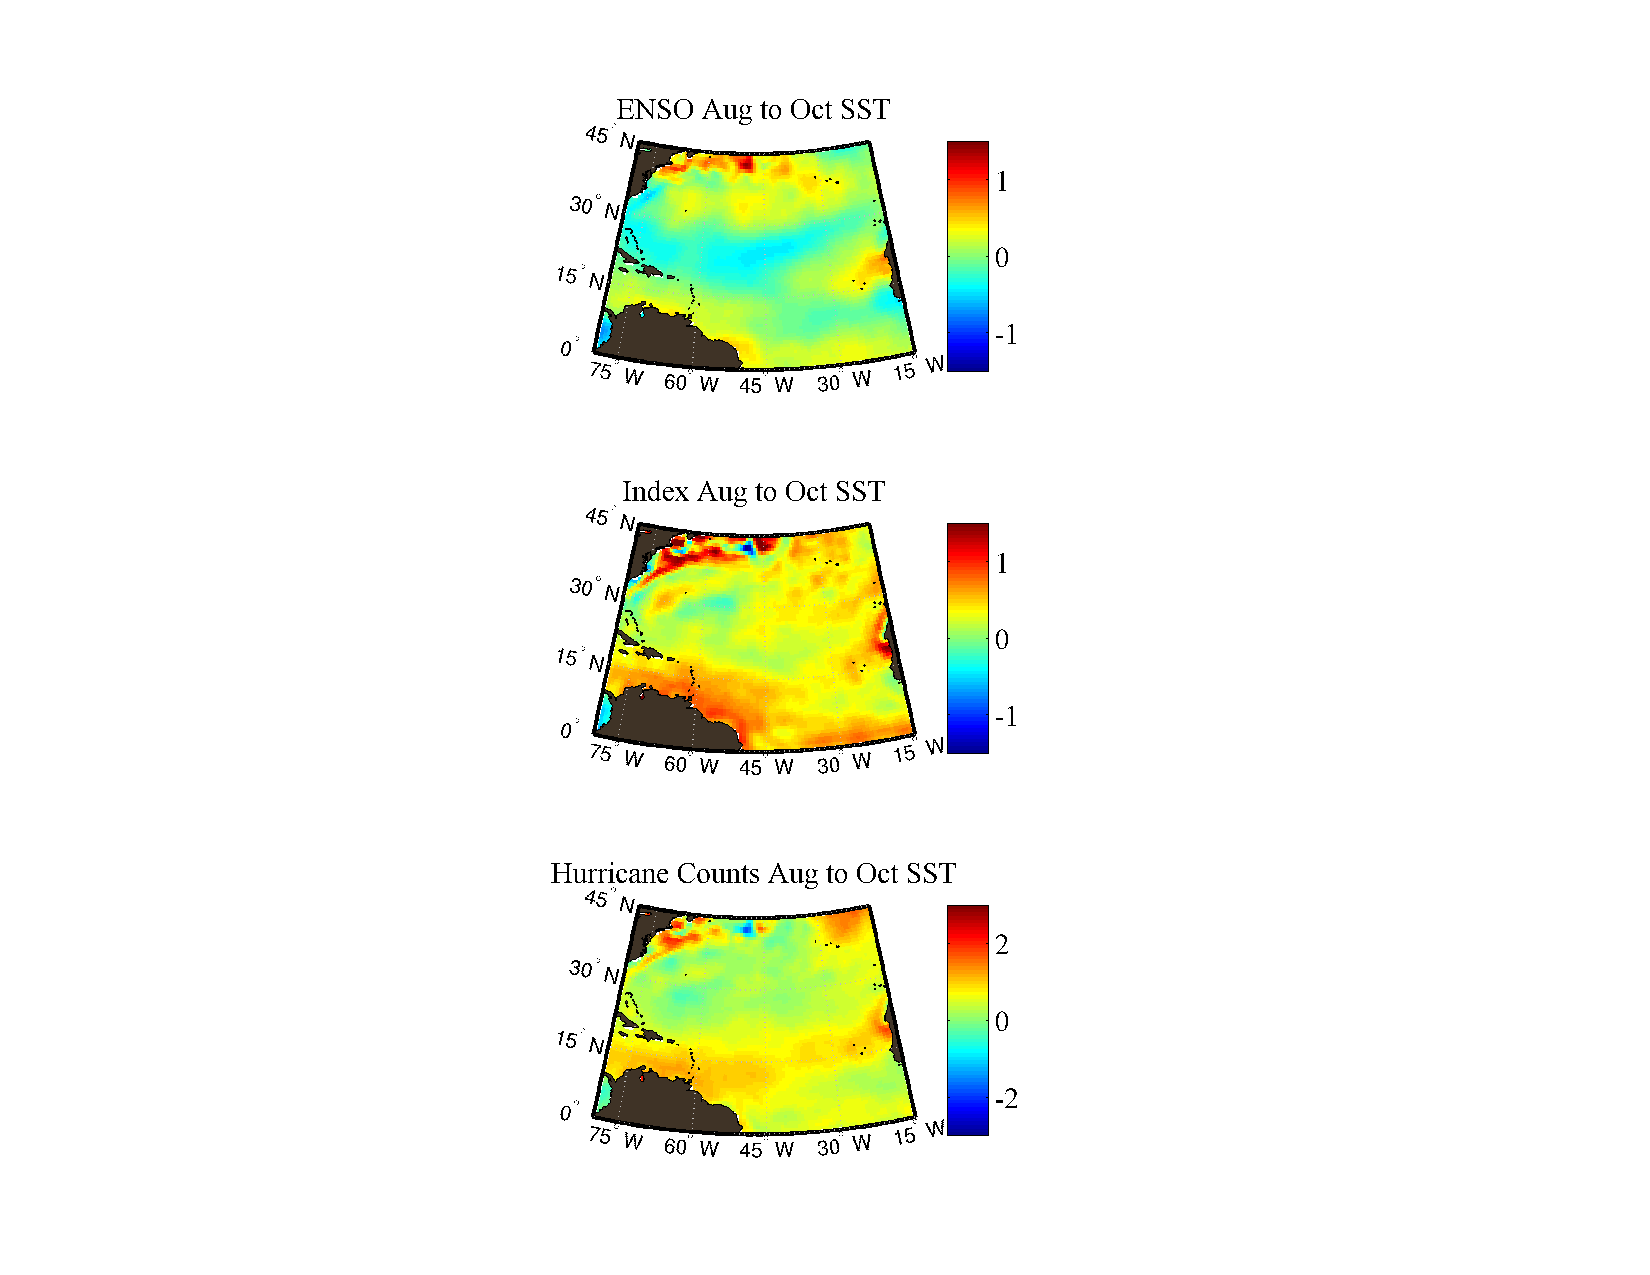
\includegraphics[width=\textwidth]{figures/sensitivityResults/compositeMaps/diffSSTCompositesAugToOct.pdf}
\caption{Diff SST Composites}
\label{fig:figure24}
\end{minipage}
\end{figure}

\pagebreak
\begin{figure}[ht]
\begin{minipage}[b]{0.6\linewidth}
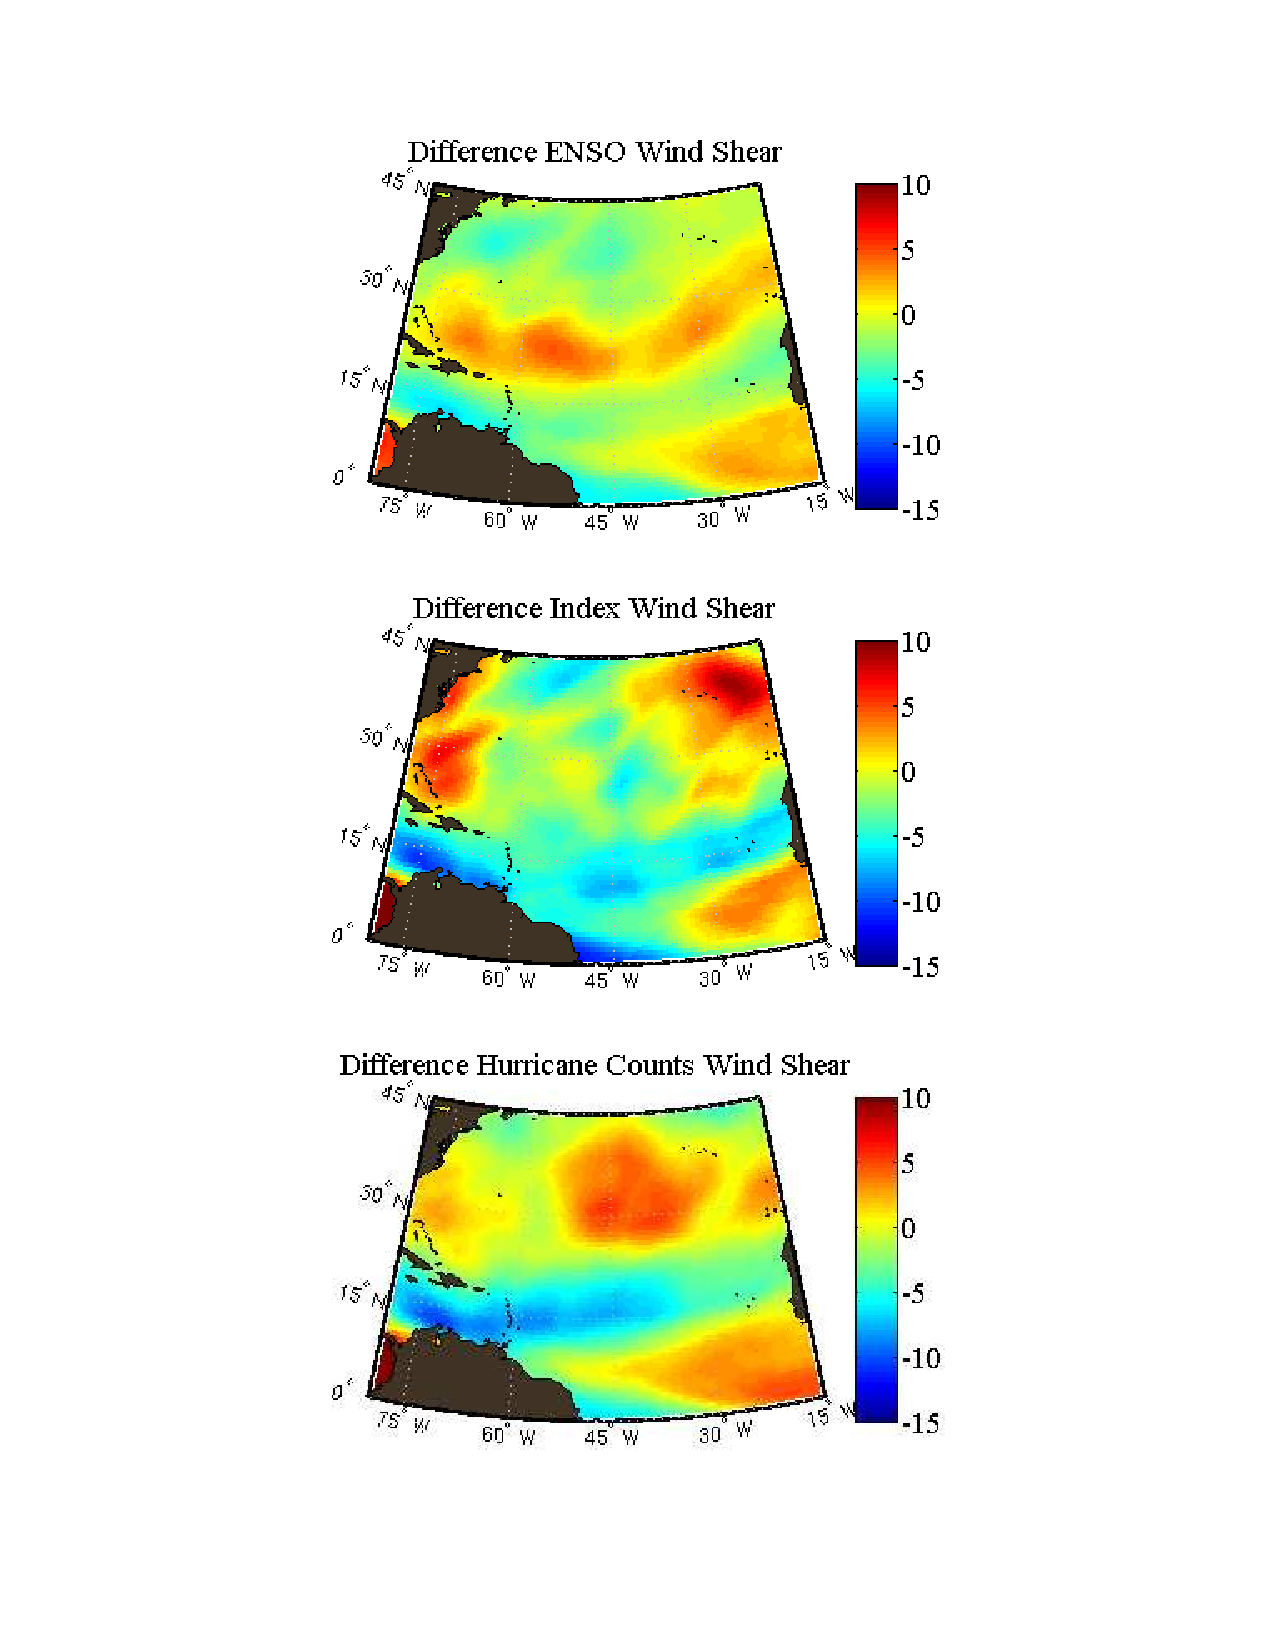
\includegraphics[width=\textwidth]{figures/sensitivityResults/compositeMaps/diffWindShearAtlanticComposites.pdf}
\caption{Diff Wind Shear}
\label{fig:figure25}
\end{minipage}
\hspace{0cm}
\begin{minipage}[b]{0.6\linewidth}
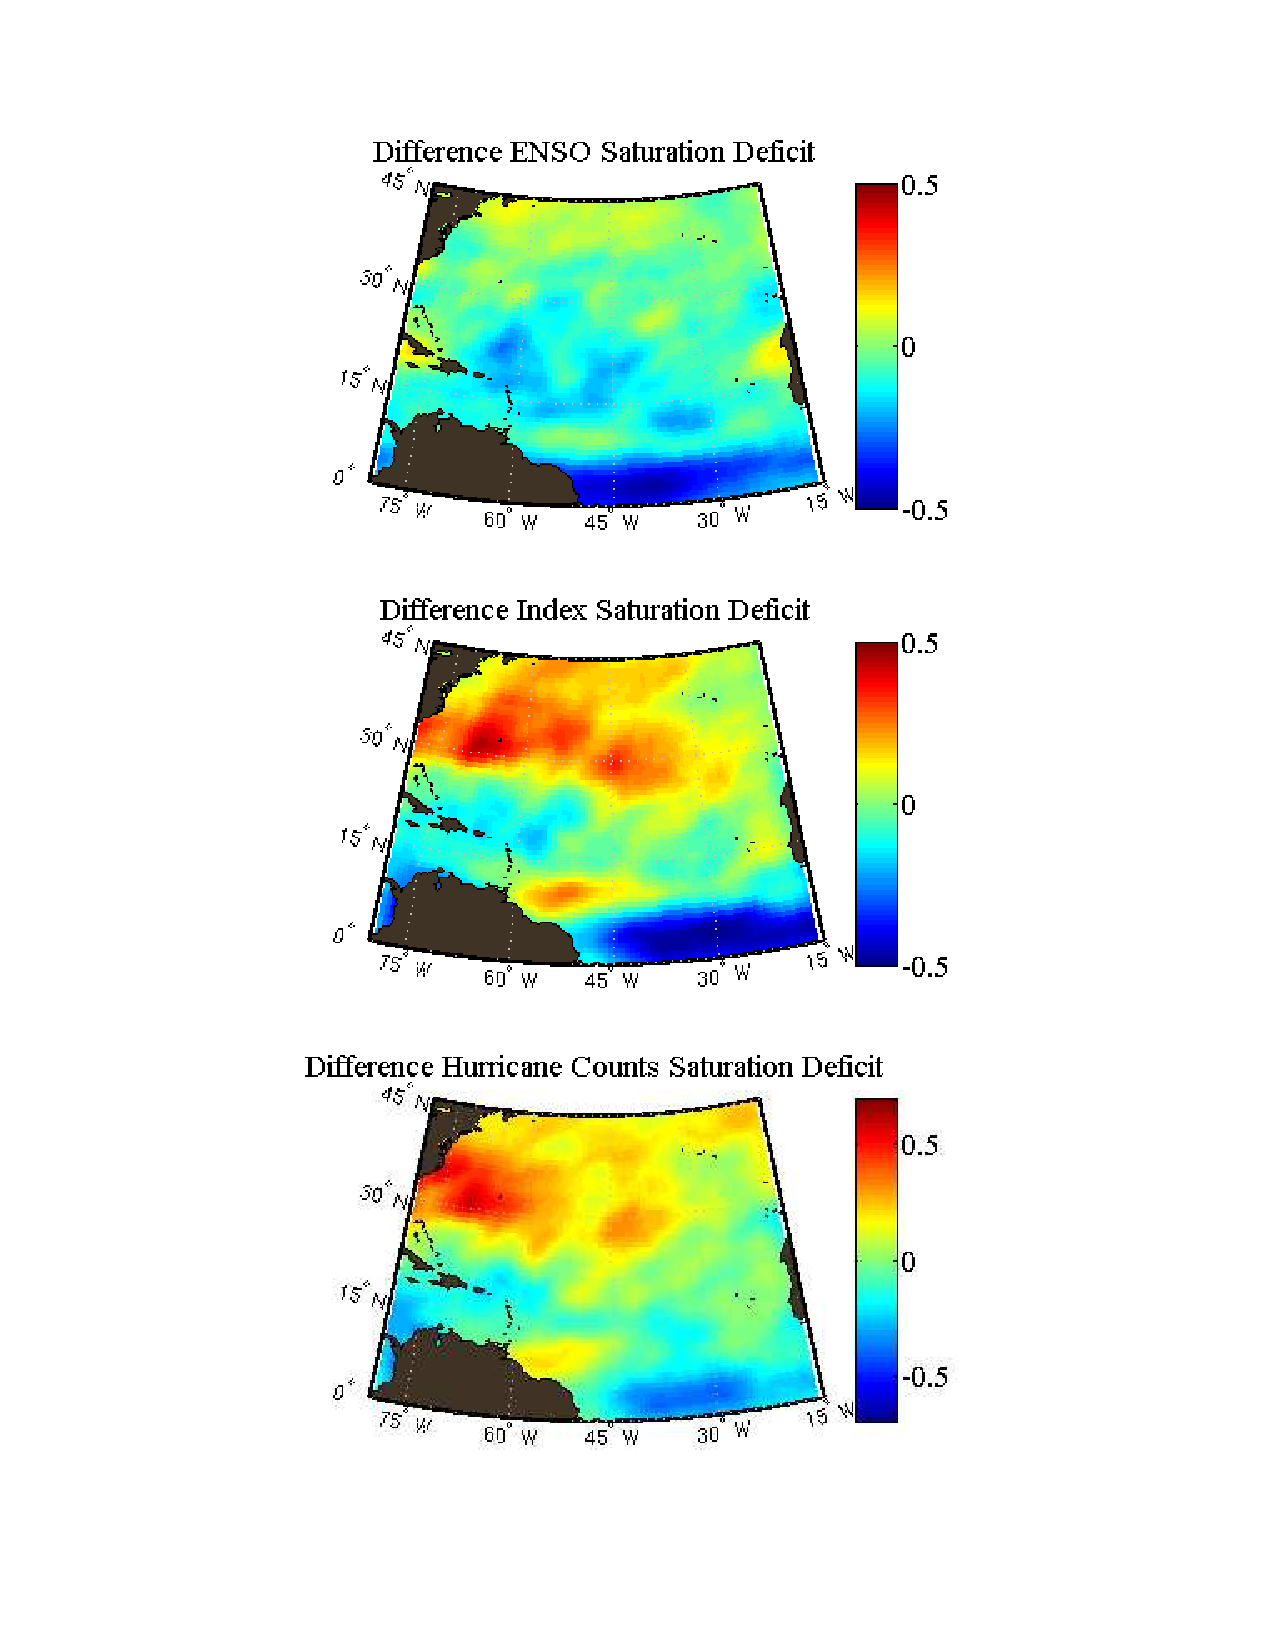
\includegraphics[width=\textwidth]{figures/sensitivityResults/compositeMaps/satDefAtlanticMap.pdf}
\caption{Diff Saturation Deficit}
\label{fig:figure26}
\end{minipage}
\end{figure}

\clearpage
\section{Average Difference Bar Graphs}
\begin{figure}[ht]
\begin{minipage}[b]{0.6\linewidth}
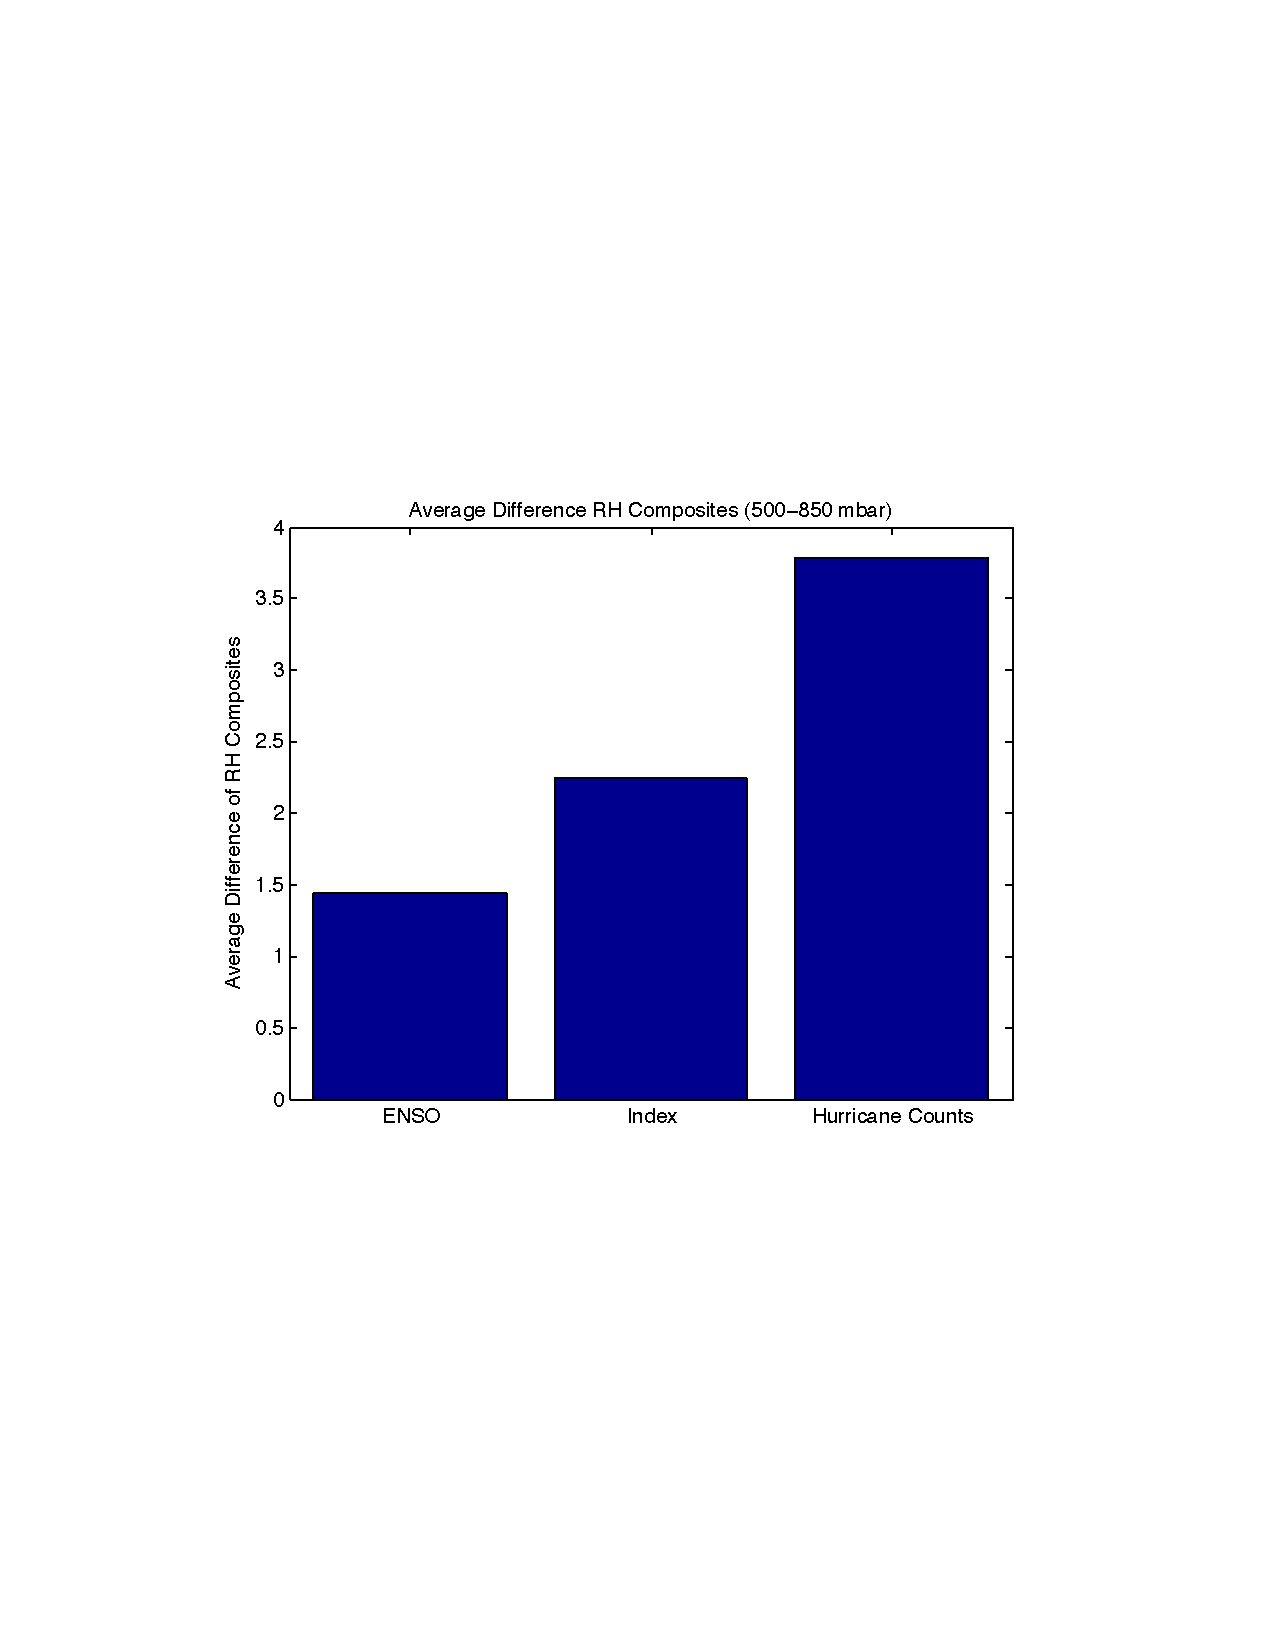
\includegraphics[width=\textwidth]{figures/sensitivityResults/compositeBarGraphs/RHBarGraph.pdf}
\caption{Avg Diff Relative Humidity}
\label{fig:figure27}
\end{minipage}
\hspace{0cm}
\begin{minipage}[b]{0.6\linewidth}
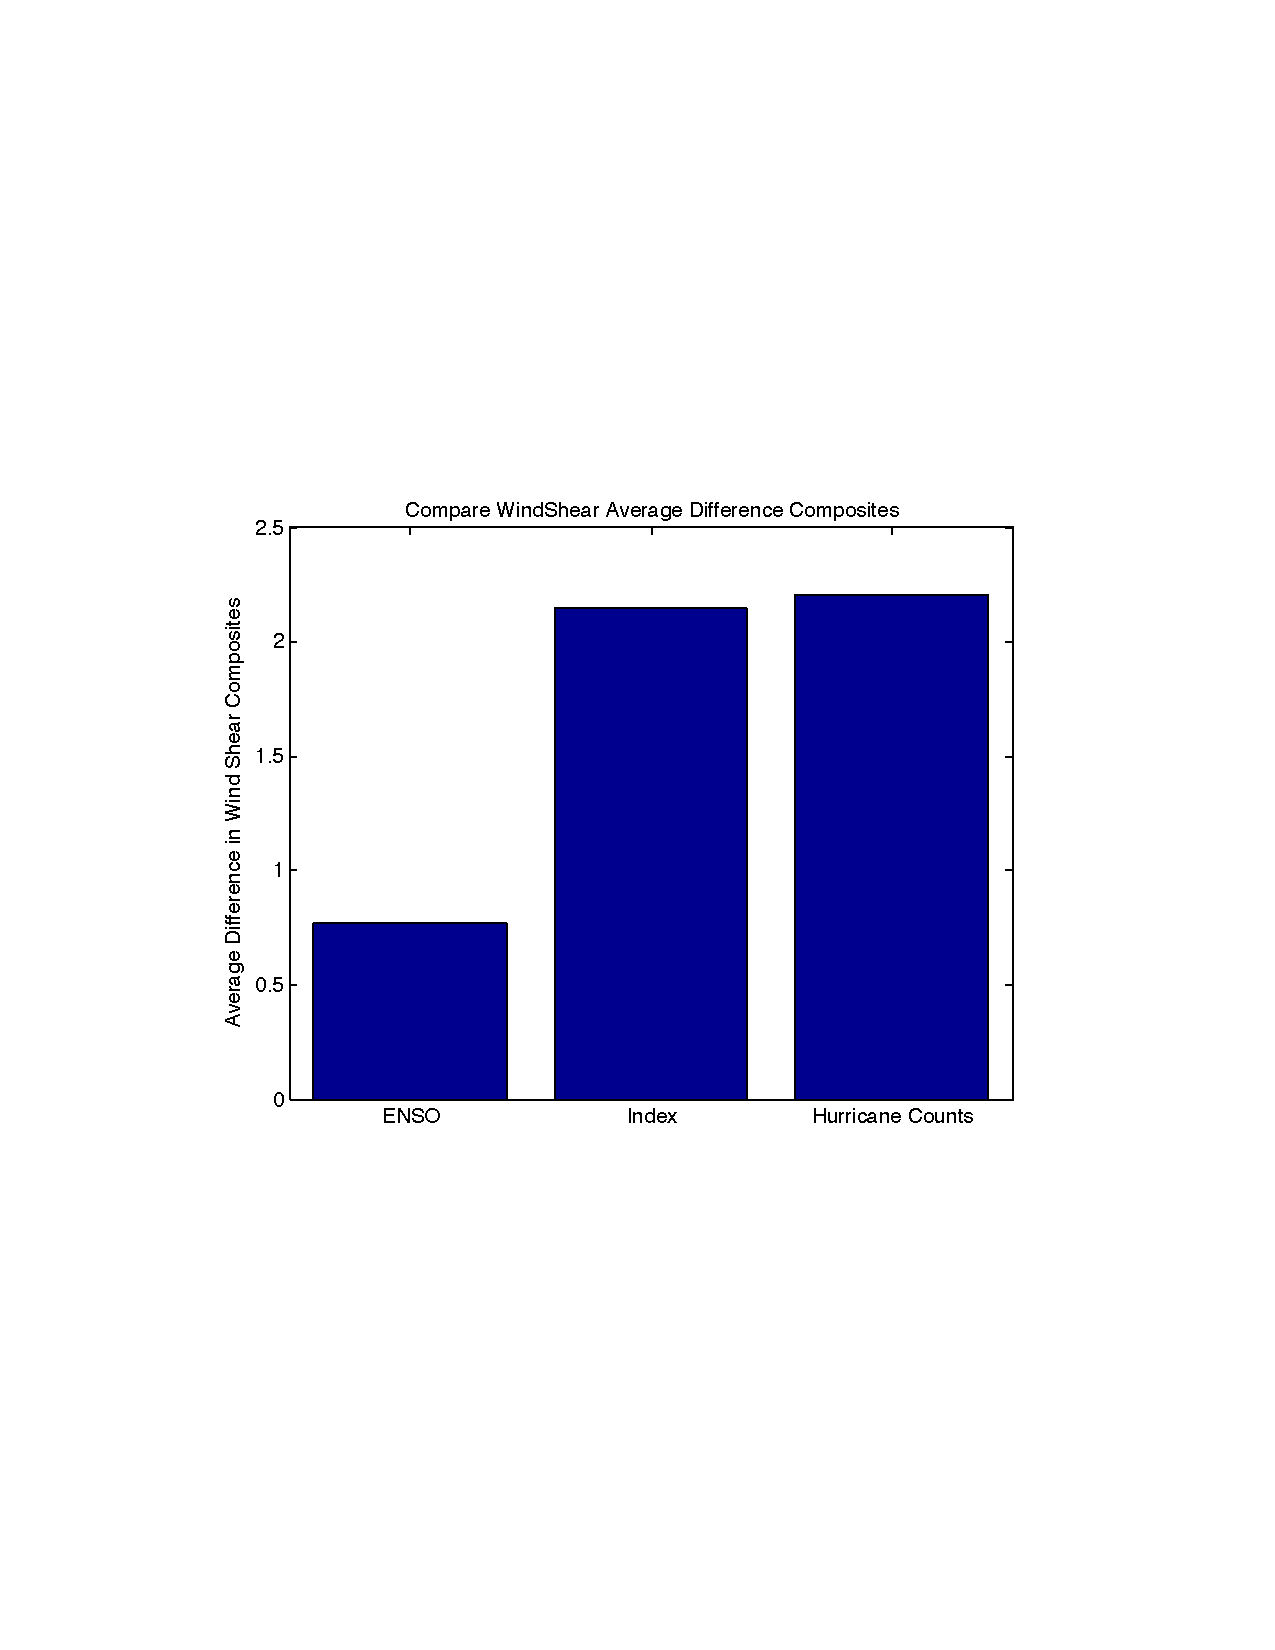
\includegraphics[width=\textwidth]{figures/sensitivityResults/compositeBarGraphs/avgDiffWindShearBarGraph.pdf}
\caption{Avg Diff Wind Shear (between 850-200mbar)}
\label{fig:figure28}
\end{minipage}
\end{figure}

\begin{figure}[ht]
\begin{minipage}[b]{0.6\linewidth}
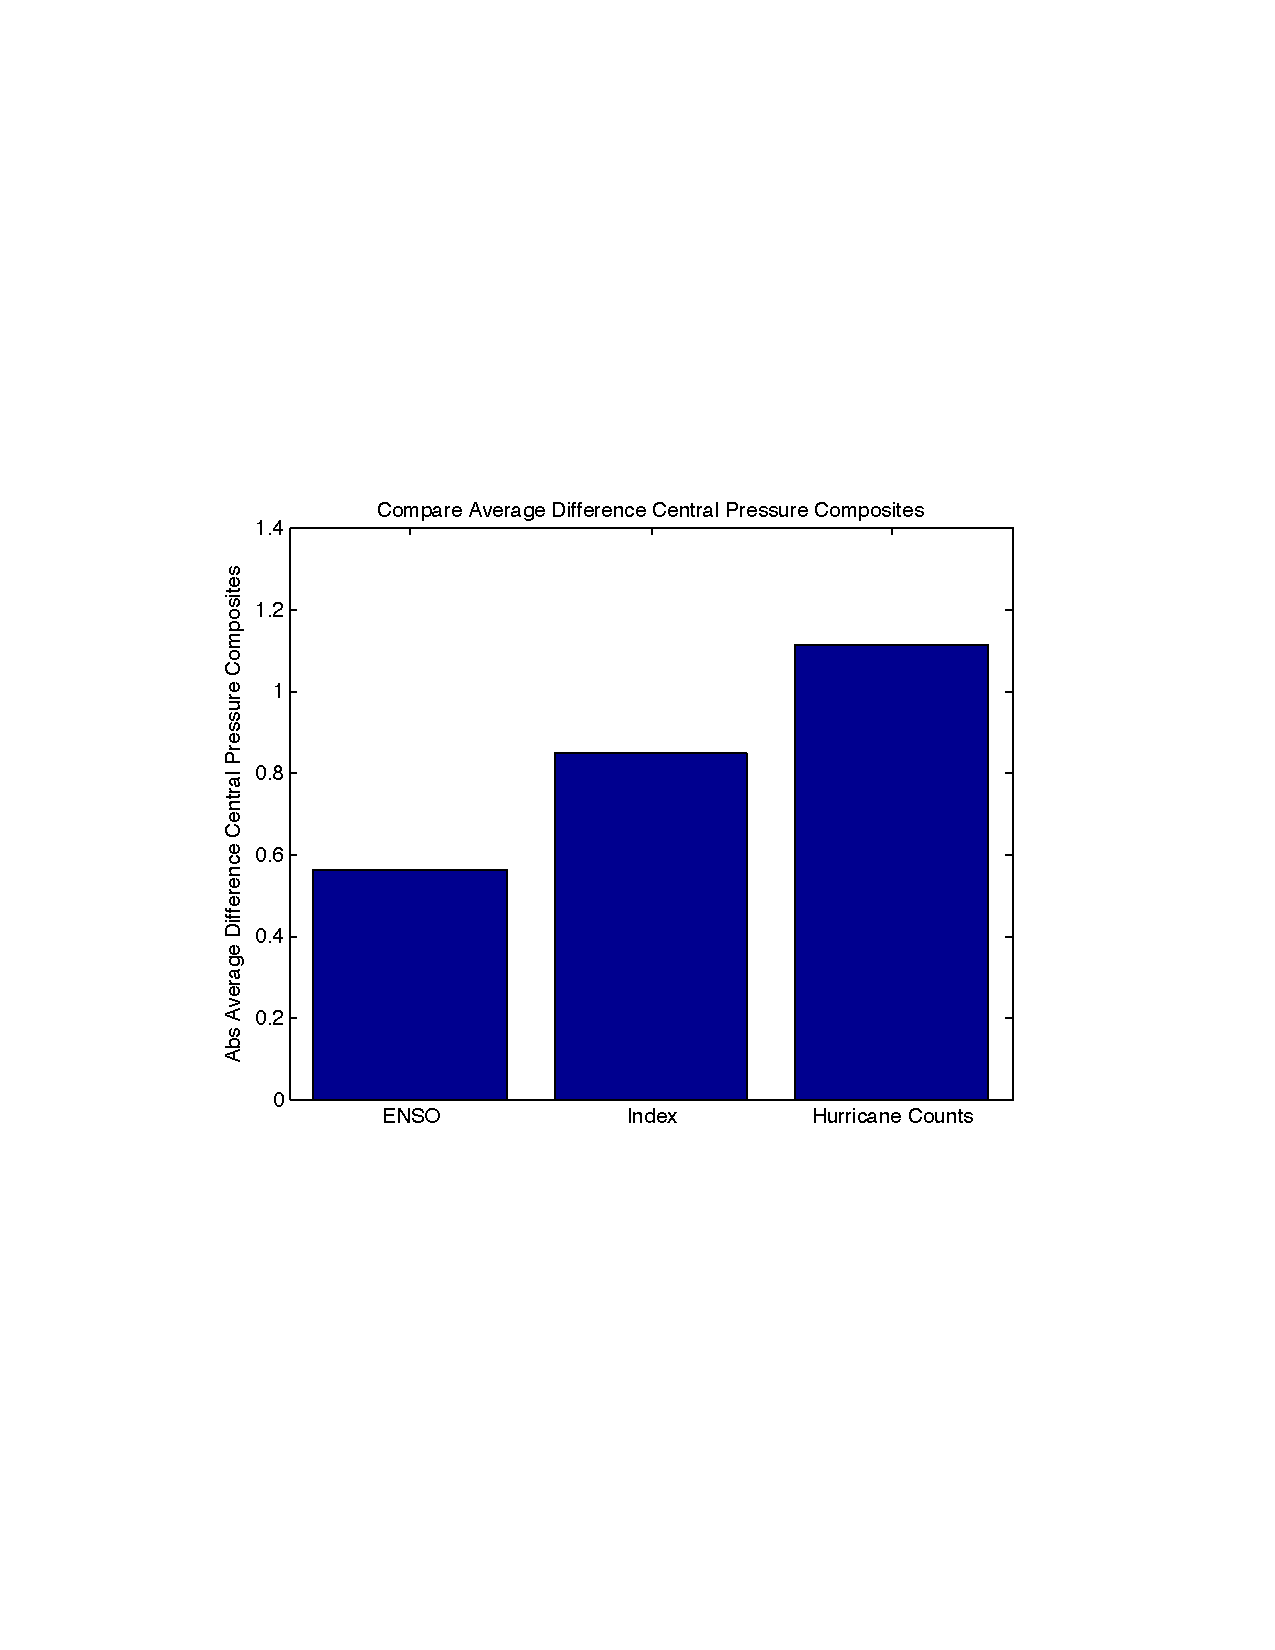
\includegraphics[width=\textwidth]{figures/sensitivityResults/compositeBarGraphs/centralPressureBarGraph.pdf}
\caption{Avg Diff Central Pressure}
\label{fig:figure29}
\end{minipage}
\hspace{0cm}
\begin{minipage}[b]{0.6\linewidth}
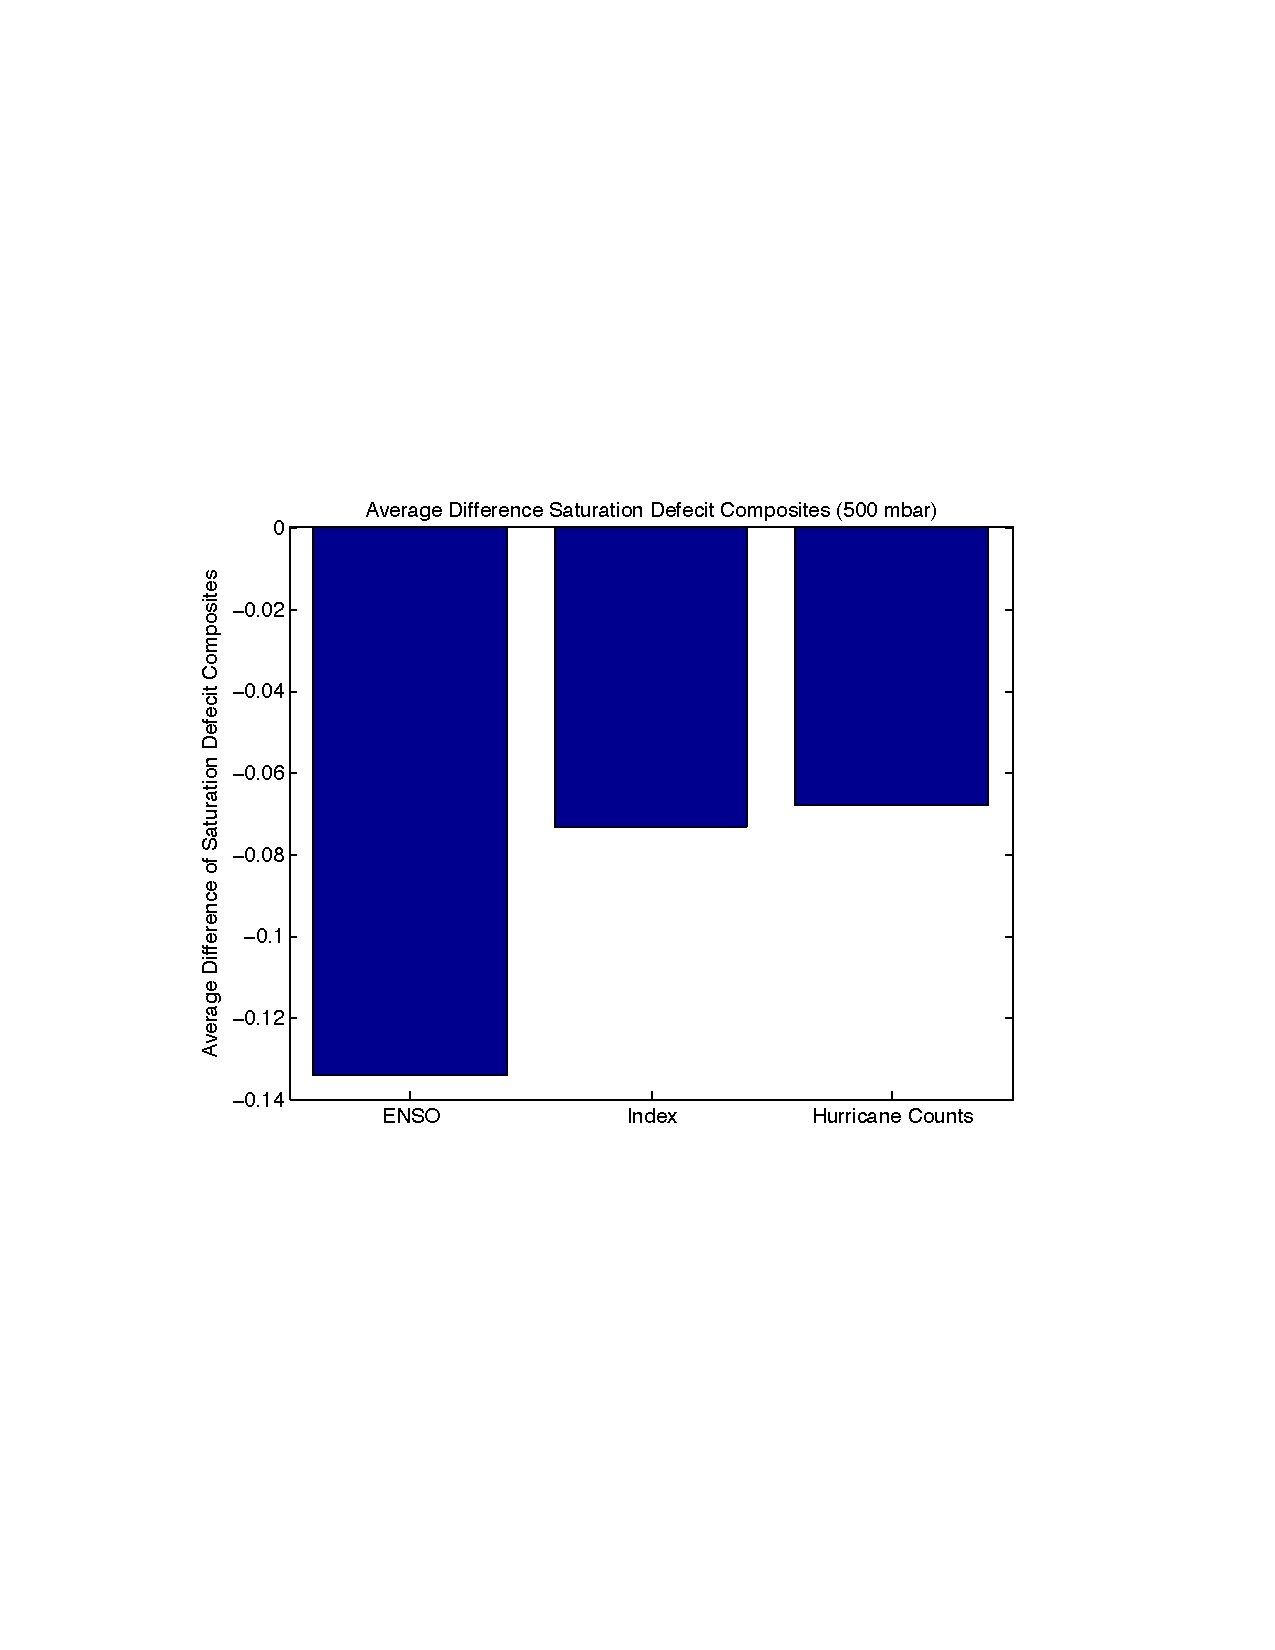
\includegraphics[width=\textwidth]{figures/sensitivityResults/compositeBarGraphs/satDefBarGraphSmallerBox.pdf}
\caption{Avg Diff Saturation Deficit}
\label{fig:figure30}
\end{minipage}
\end{figure}
\pagebreak
\begin{figure}[ht]
\begin{minipage}[b]{0.6\linewidth}
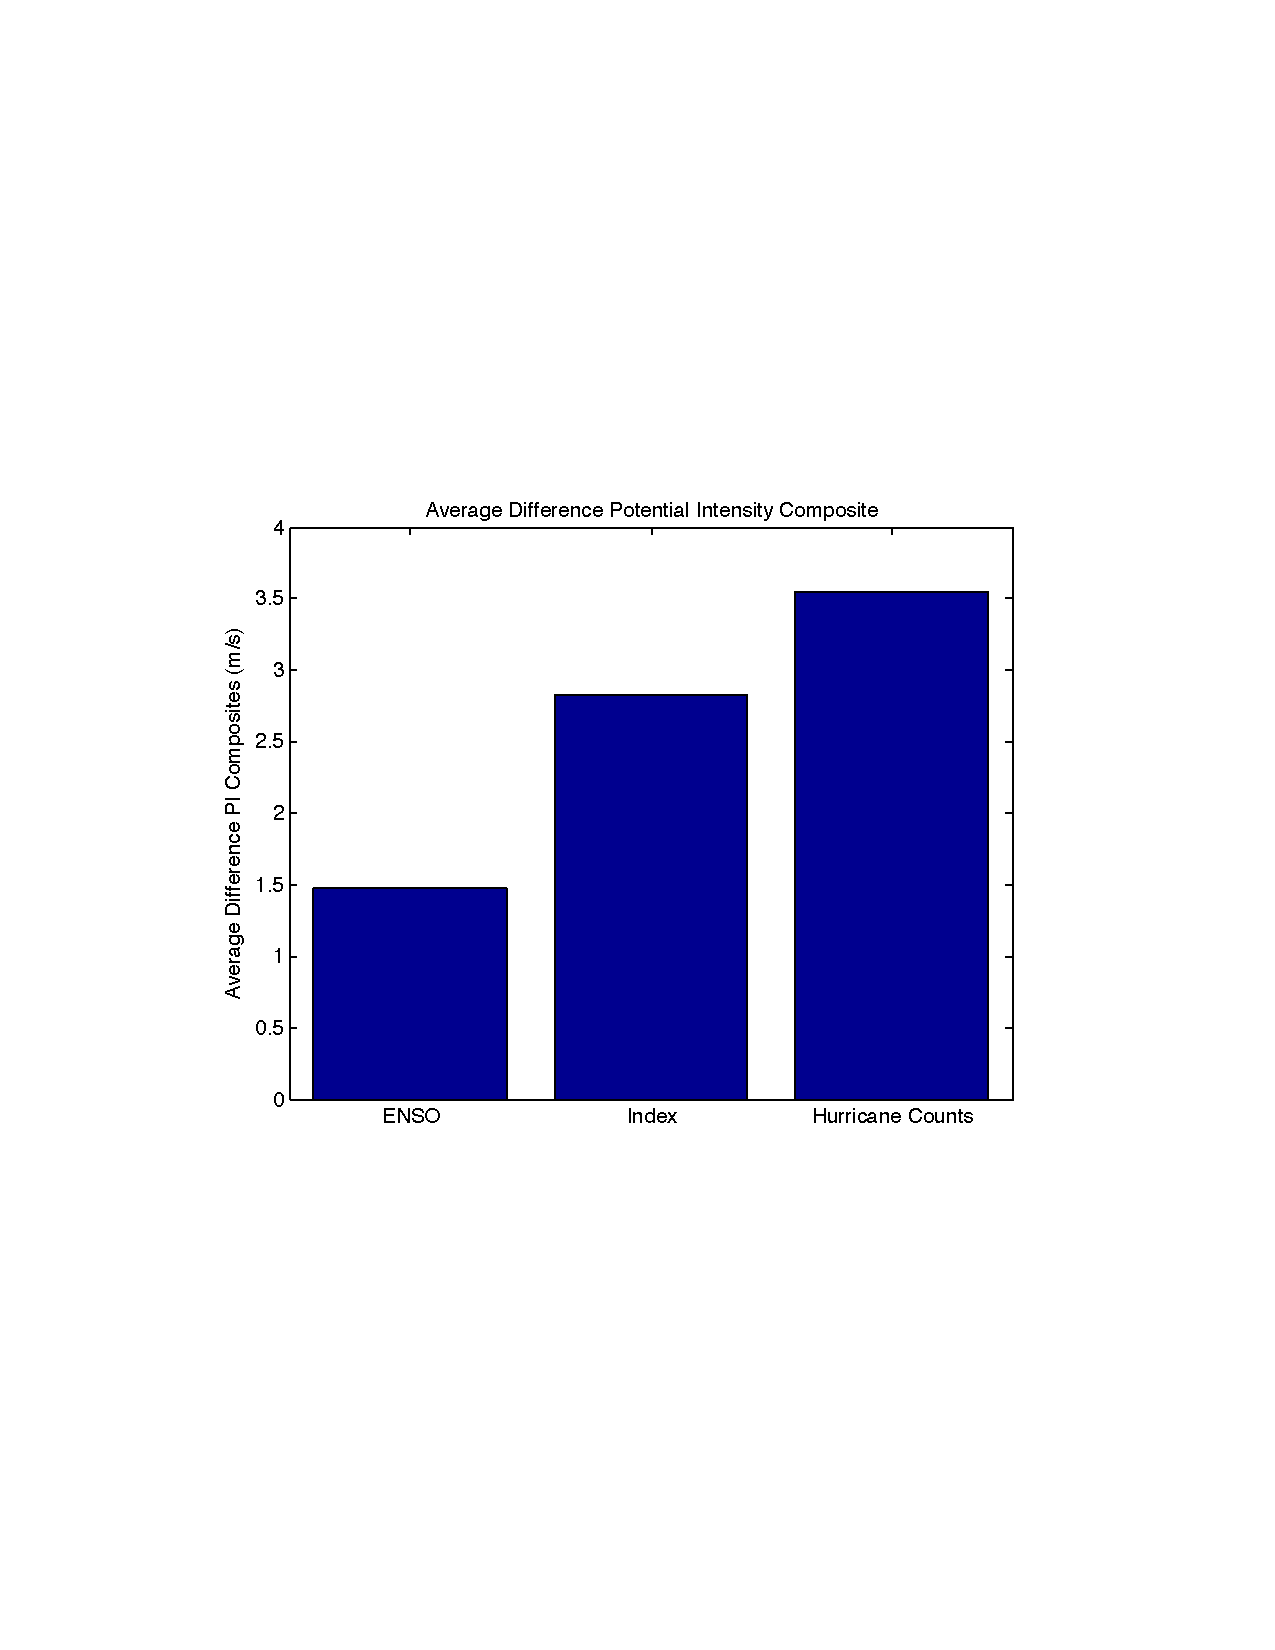
\includegraphics[width=\textwidth]{figures/sensitivityResults/compositeBarGraphs/avgDiffPIAtlanticCompositesBarGraph.pdf}
\caption{Avg Diff Potential Intensity}
\label{fig:figure31}
\end{minipage}
\hspace{0cm}
\begin{minipage}[b]{0.6\linewidth}
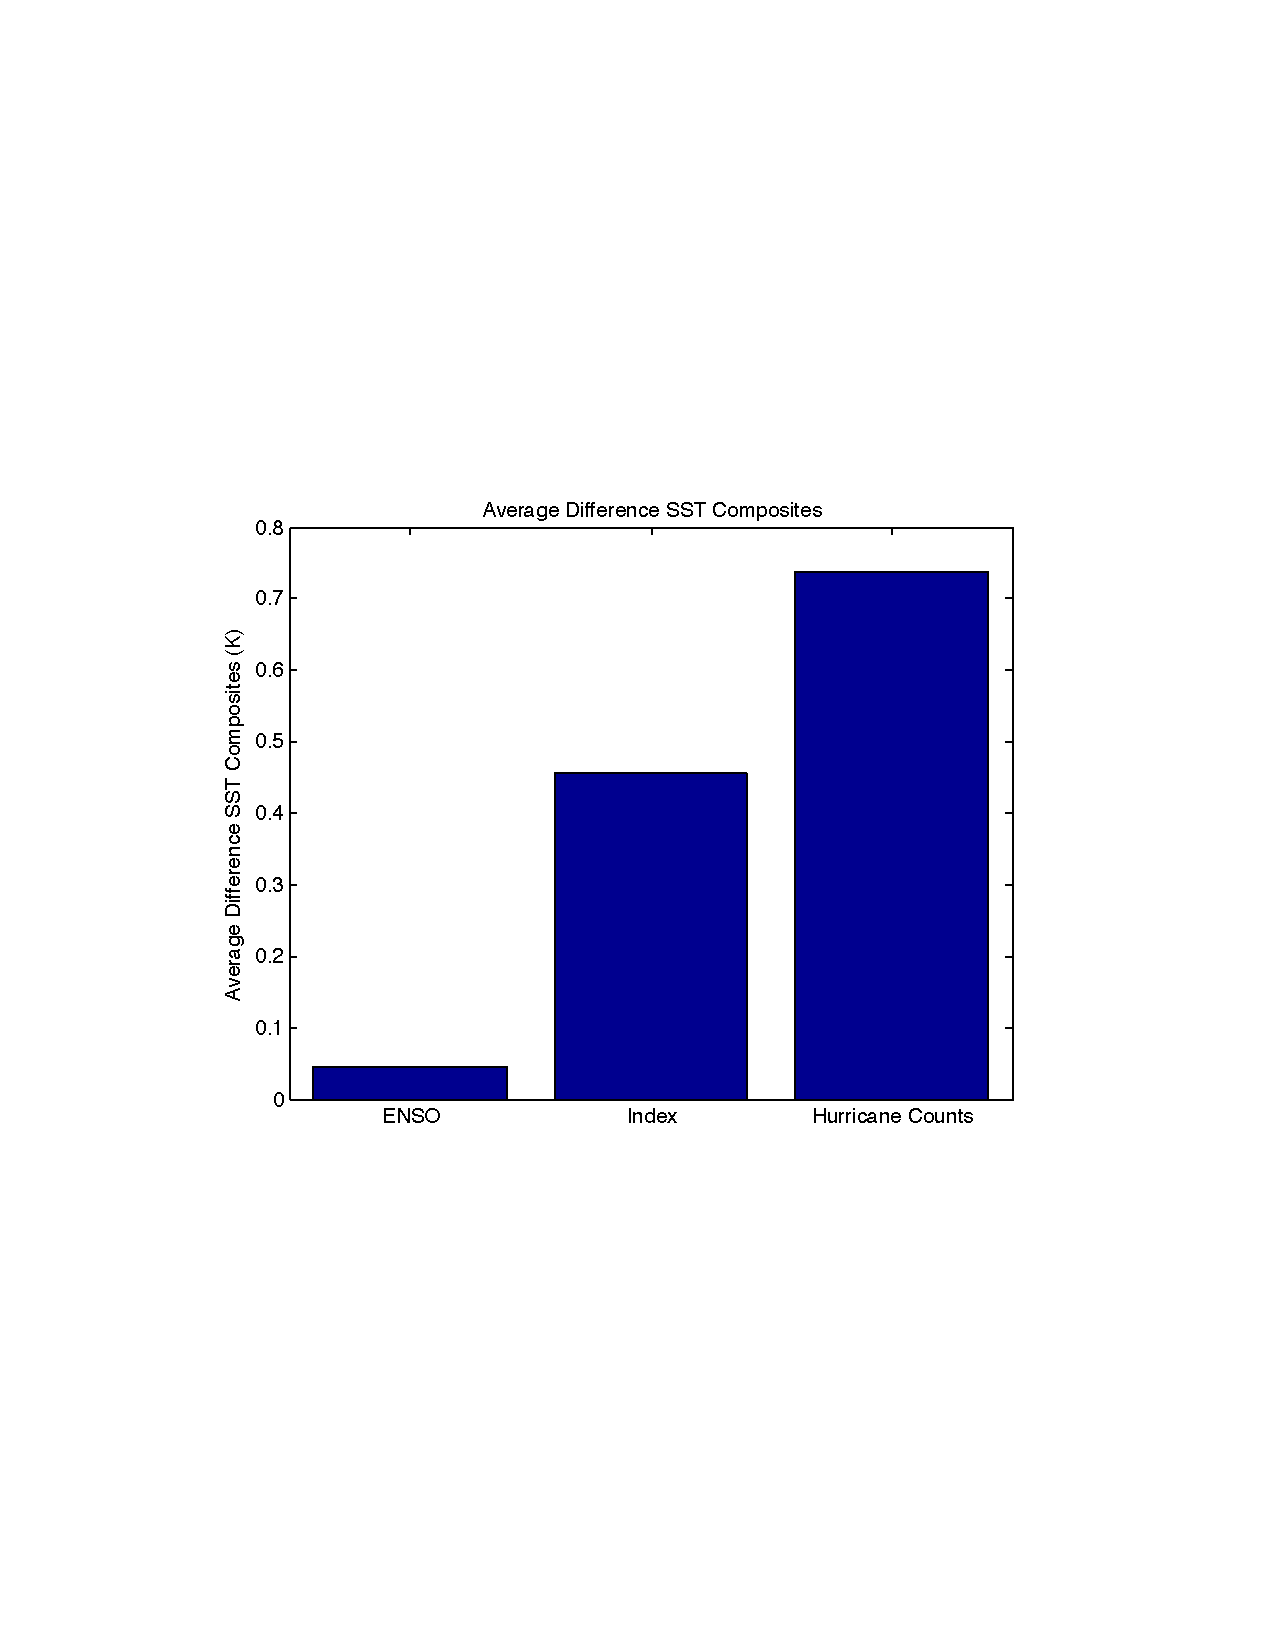
\includegraphics[width=\textwidth]{figures/sensitivityResults/compositeBarGraphs/sstBarGraph.pdf}
\caption{Avg Diff SST}
\label{fig:figure32}
\end{minipage}
\end{figure}

\section{Combination Index Composites}
In this section, we compute four different indices, take the z-score of each, and then sum all of them up into one index.  The four indices are: the OLR value inside the box of the warmest SST box, the pressure value inside of the warmest SST box, the longitude of the box with the lowest pressure, and the longitudinal distance between the warmest SST box and the coolest SST box.  In this section we should the results where we get the years of the highest index, composite 5 different variables, do the same for the years of low index, and then subtract the composites.
\newpage

\begin{figure}[ht]
\begin{minipage}[b]{0.55\linewidth}
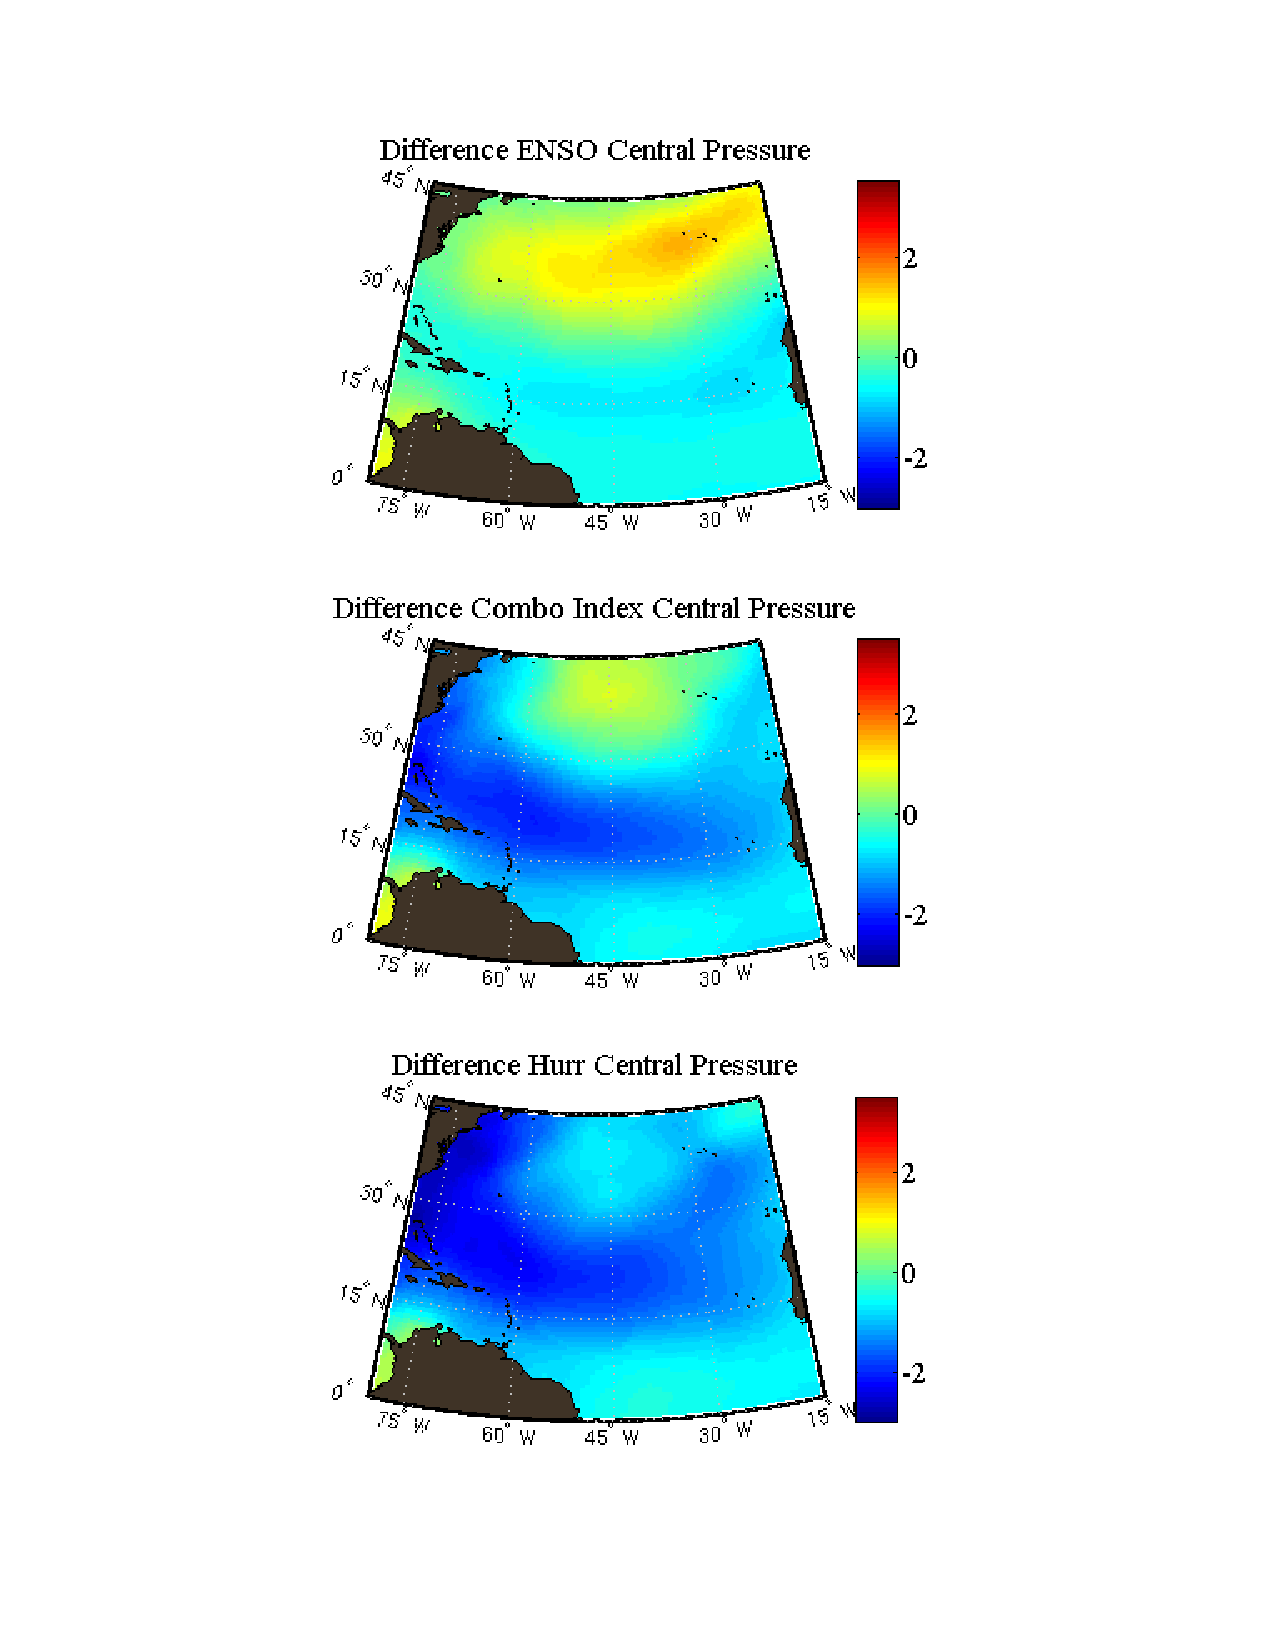
\includegraphics[width=\textwidth]{figures/comboIndex/composites/compareMDRCompositesCentralPressure.pdf}
\caption{Diff Pressure Composites}
\label{fig:figure21}
\end{minipage}
\hspace{0cm}
\begin{minipage}[b]{0.55\linewidth}
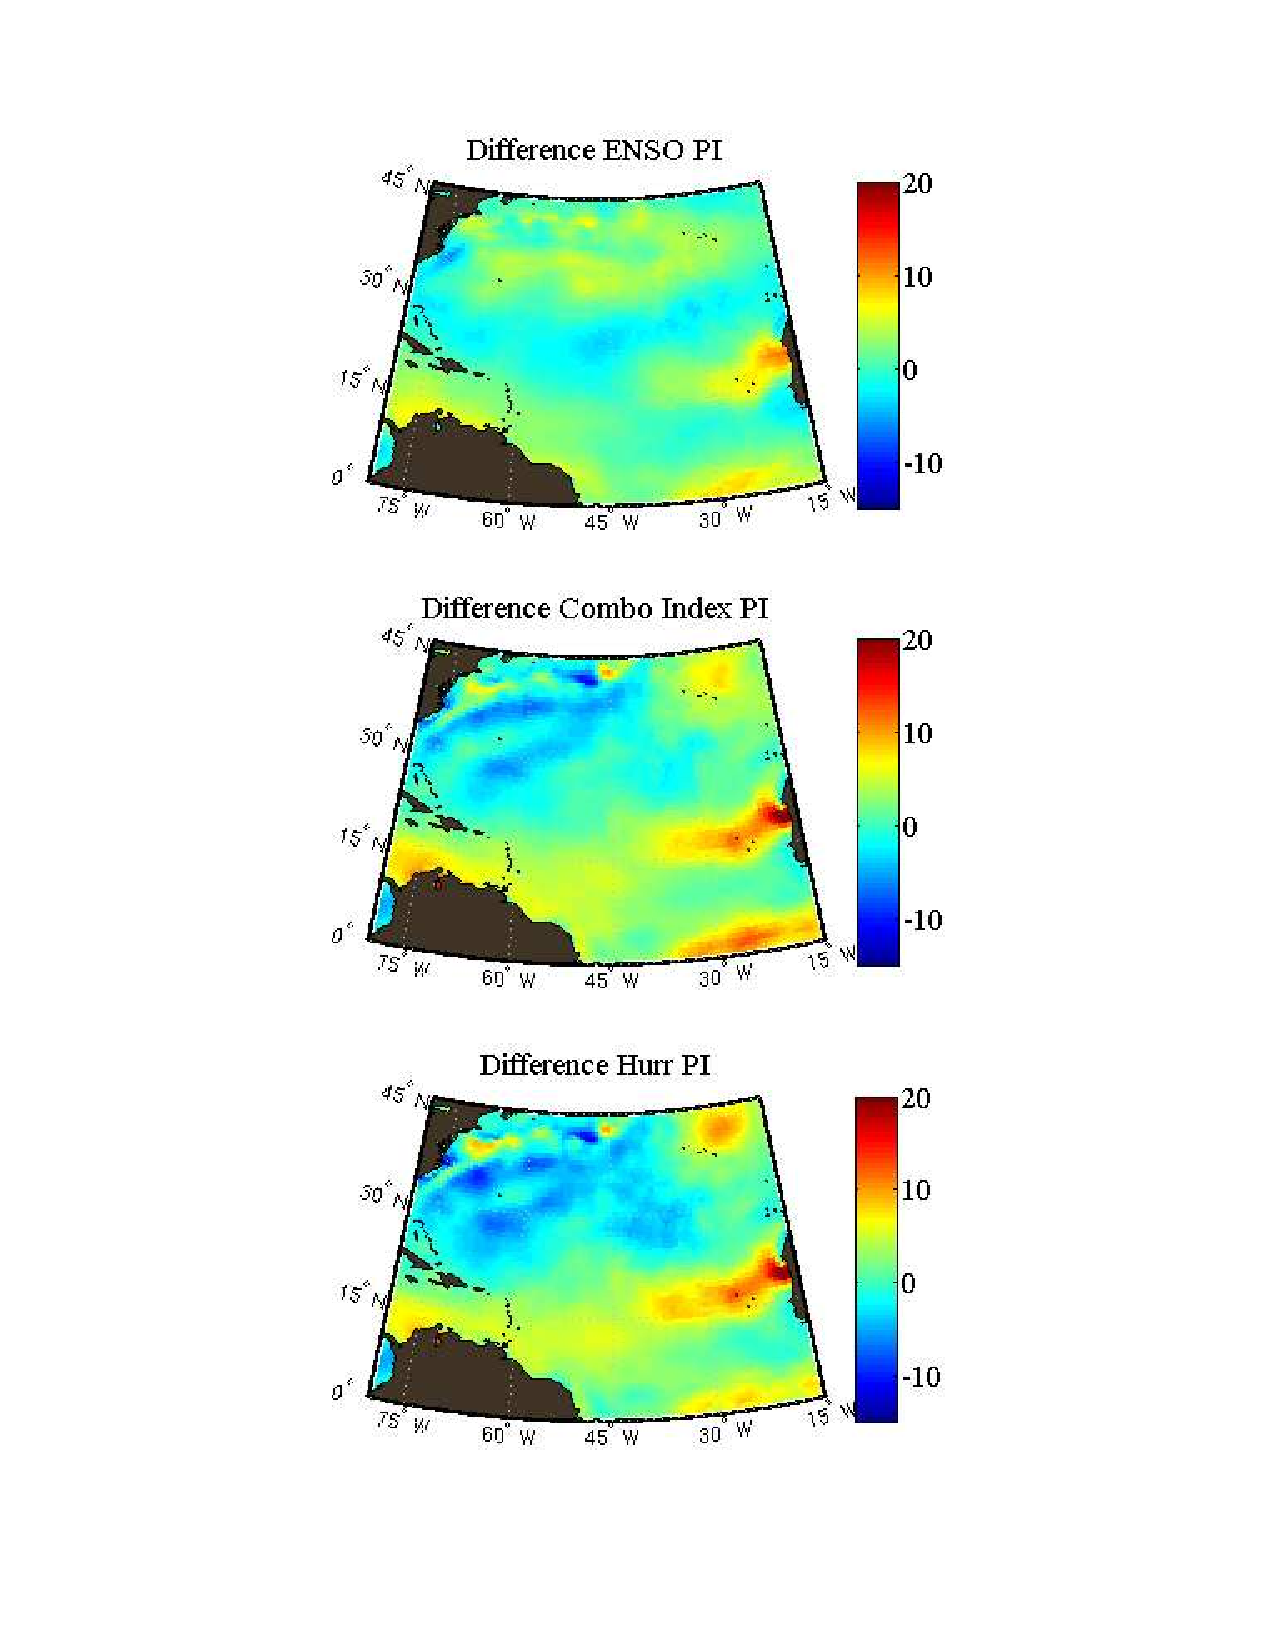
\includegraphics[width=\textwidth]{figures/comboIndex/composites/compareMDRCompositesPI.pdf}
\caption{Diff PI Composites}
\label{fig:figure22}
\end{minipage}
\end{figure}


\begin{figure}[ht]
\begin{minipage}[b]{0.55\linewidth}
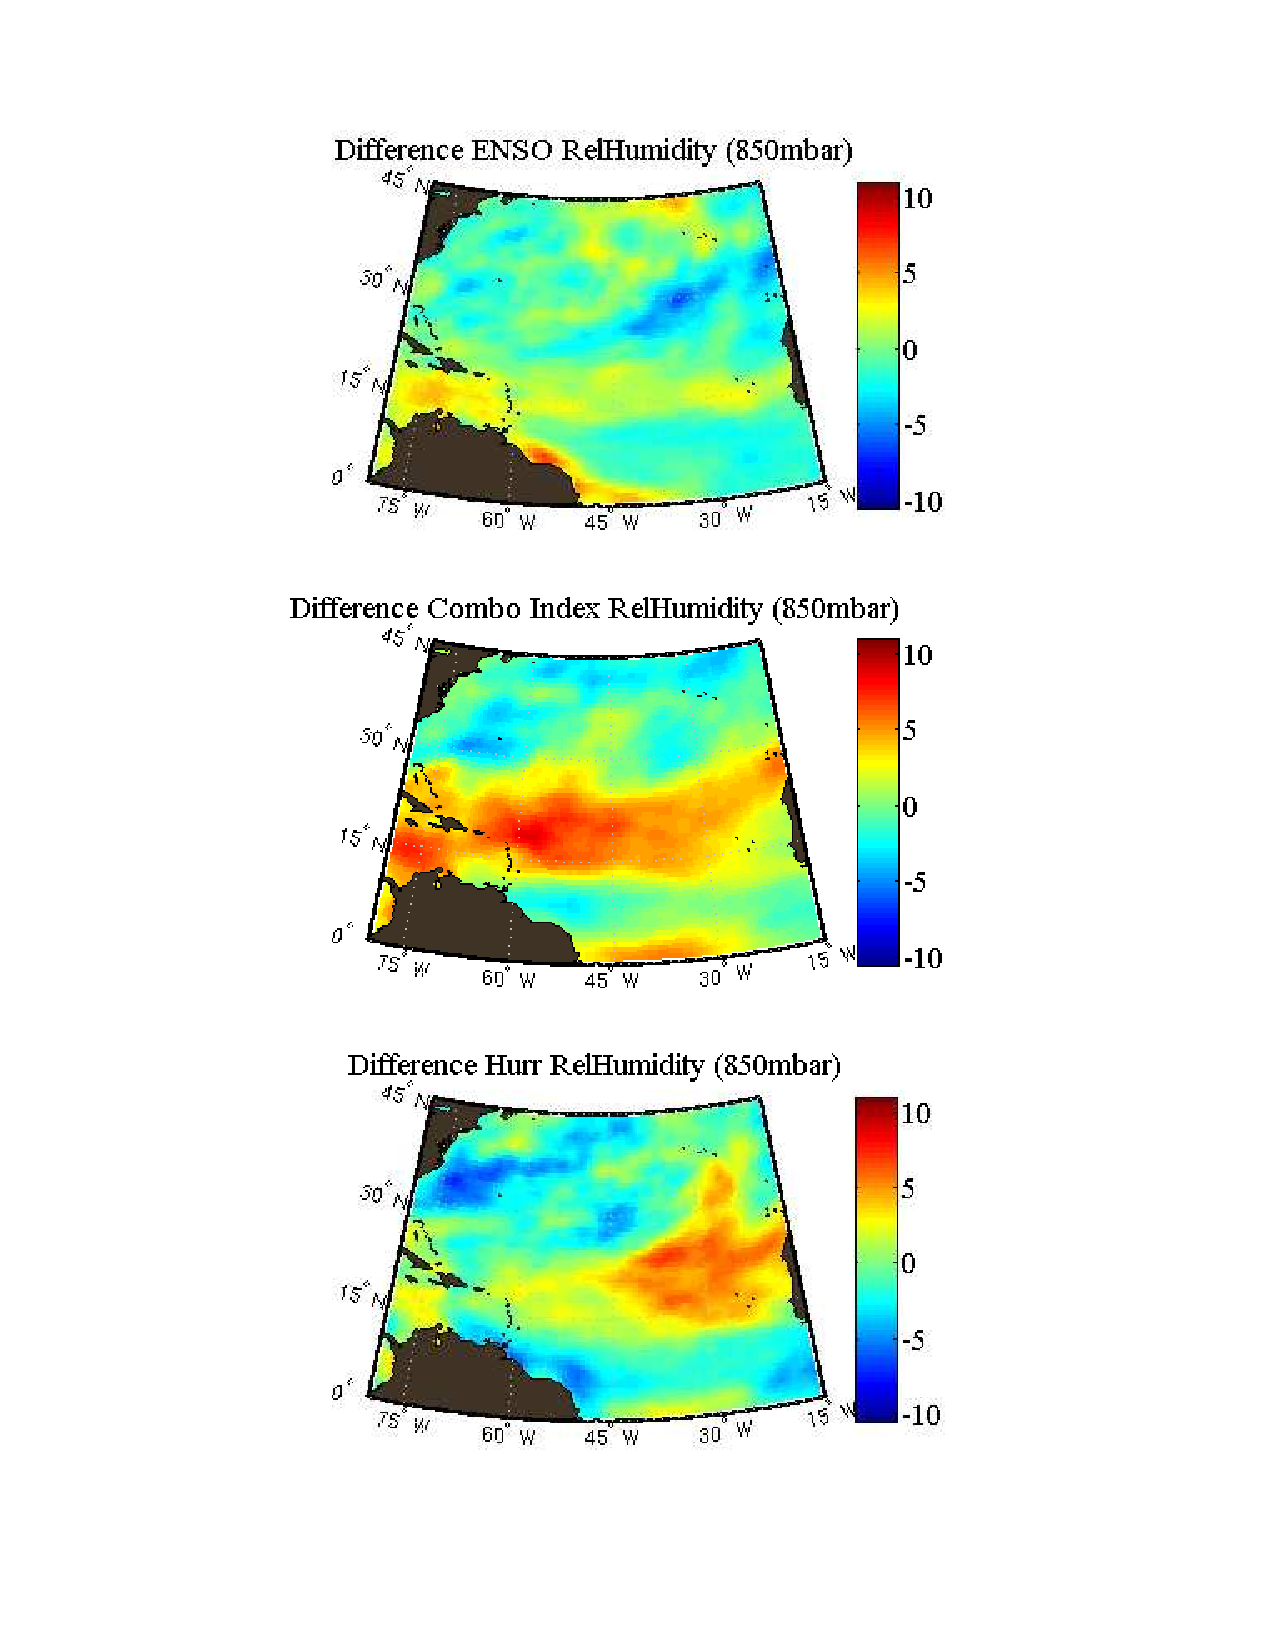
\includegraphics[width=\textwidth]{figures/comboIndex/composites/compareMDRCompositesRelativeHumidity.pdf}
\caption{Diff Relative Humidity 850 mbar}
\label{fig:figure21}
\end{minipage}
\hspace{0cm}
\begin{minipage}[b]{0.55\linewidth}
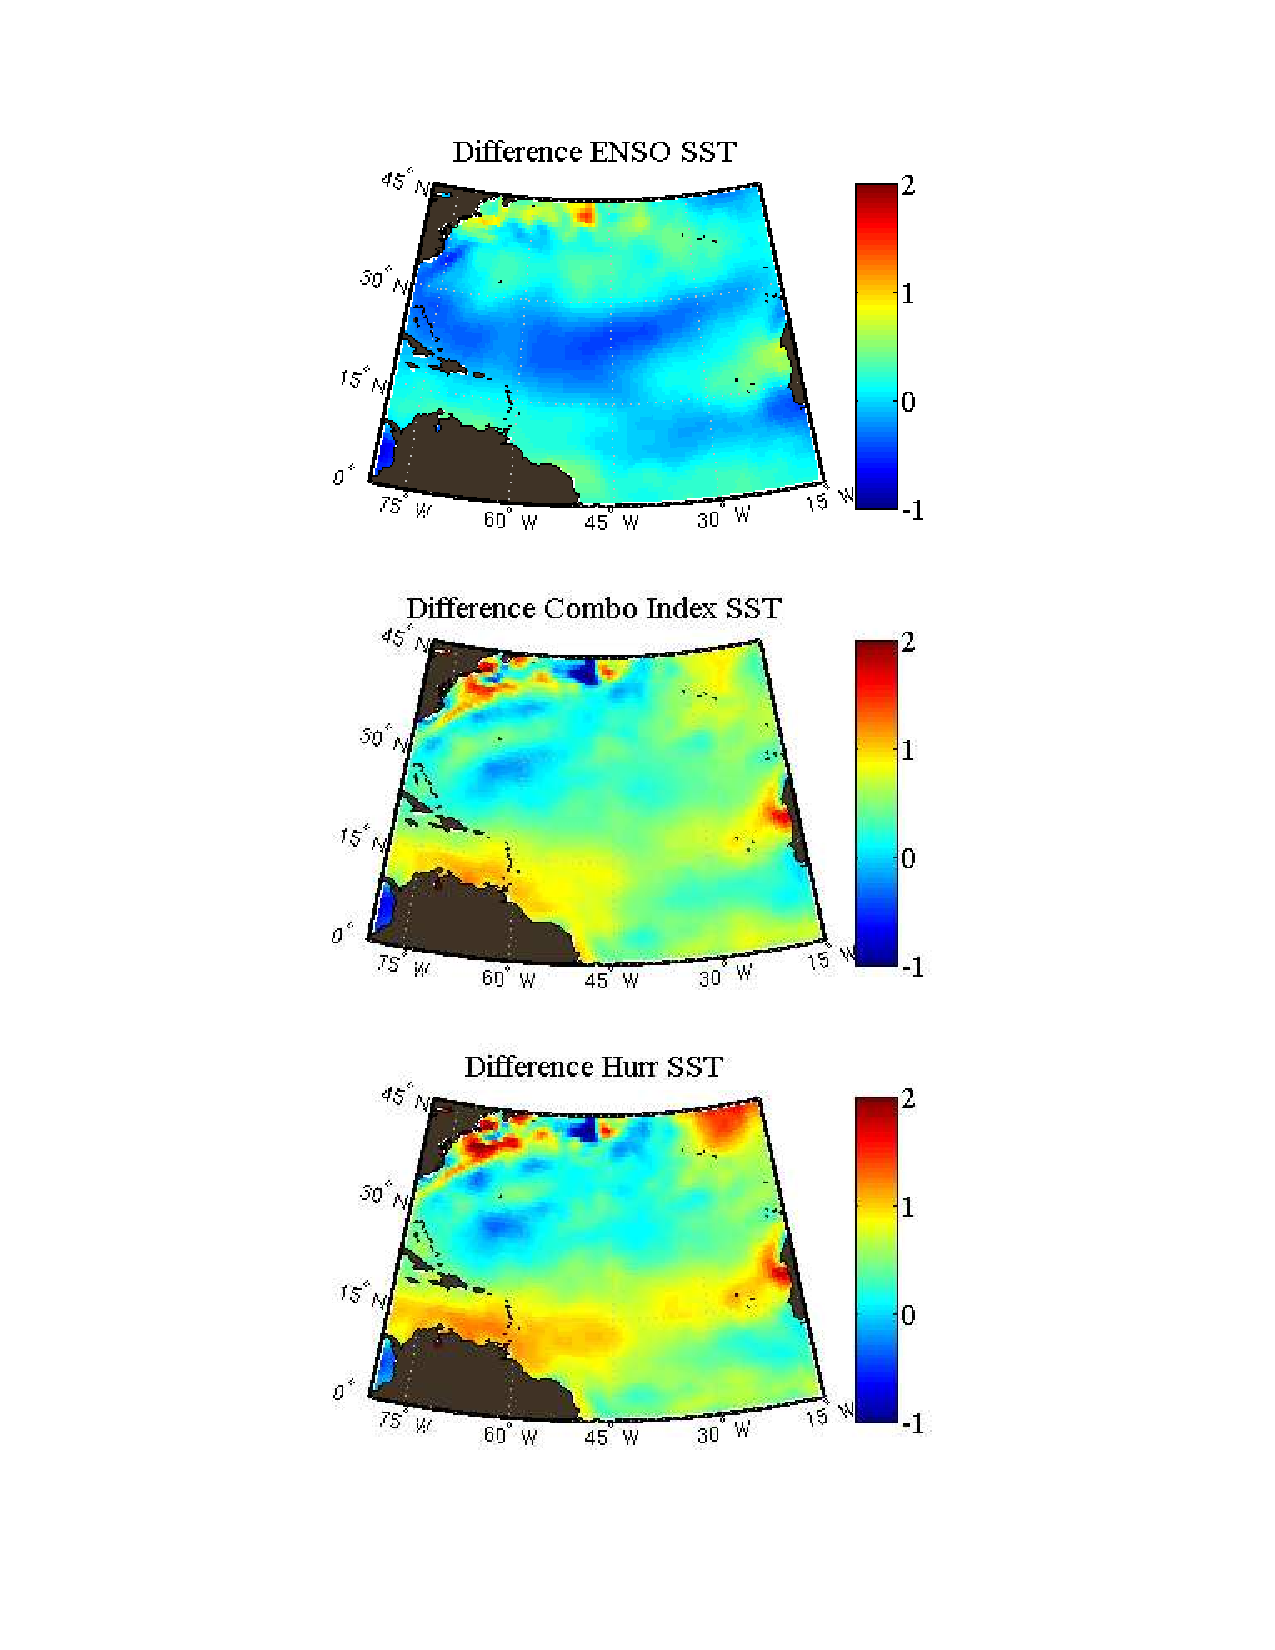
\includegraphics[width=\textwidth]{figures/comboIndex/composites/compareMDRCompositesSST.pdf}
\caption{Diff SST Composites}
\label{fig:figure22}
\end{minipage}
\end{figure}

\begin{figure}[ht]
\begin{minipage}[b]{0.55\linewidth}
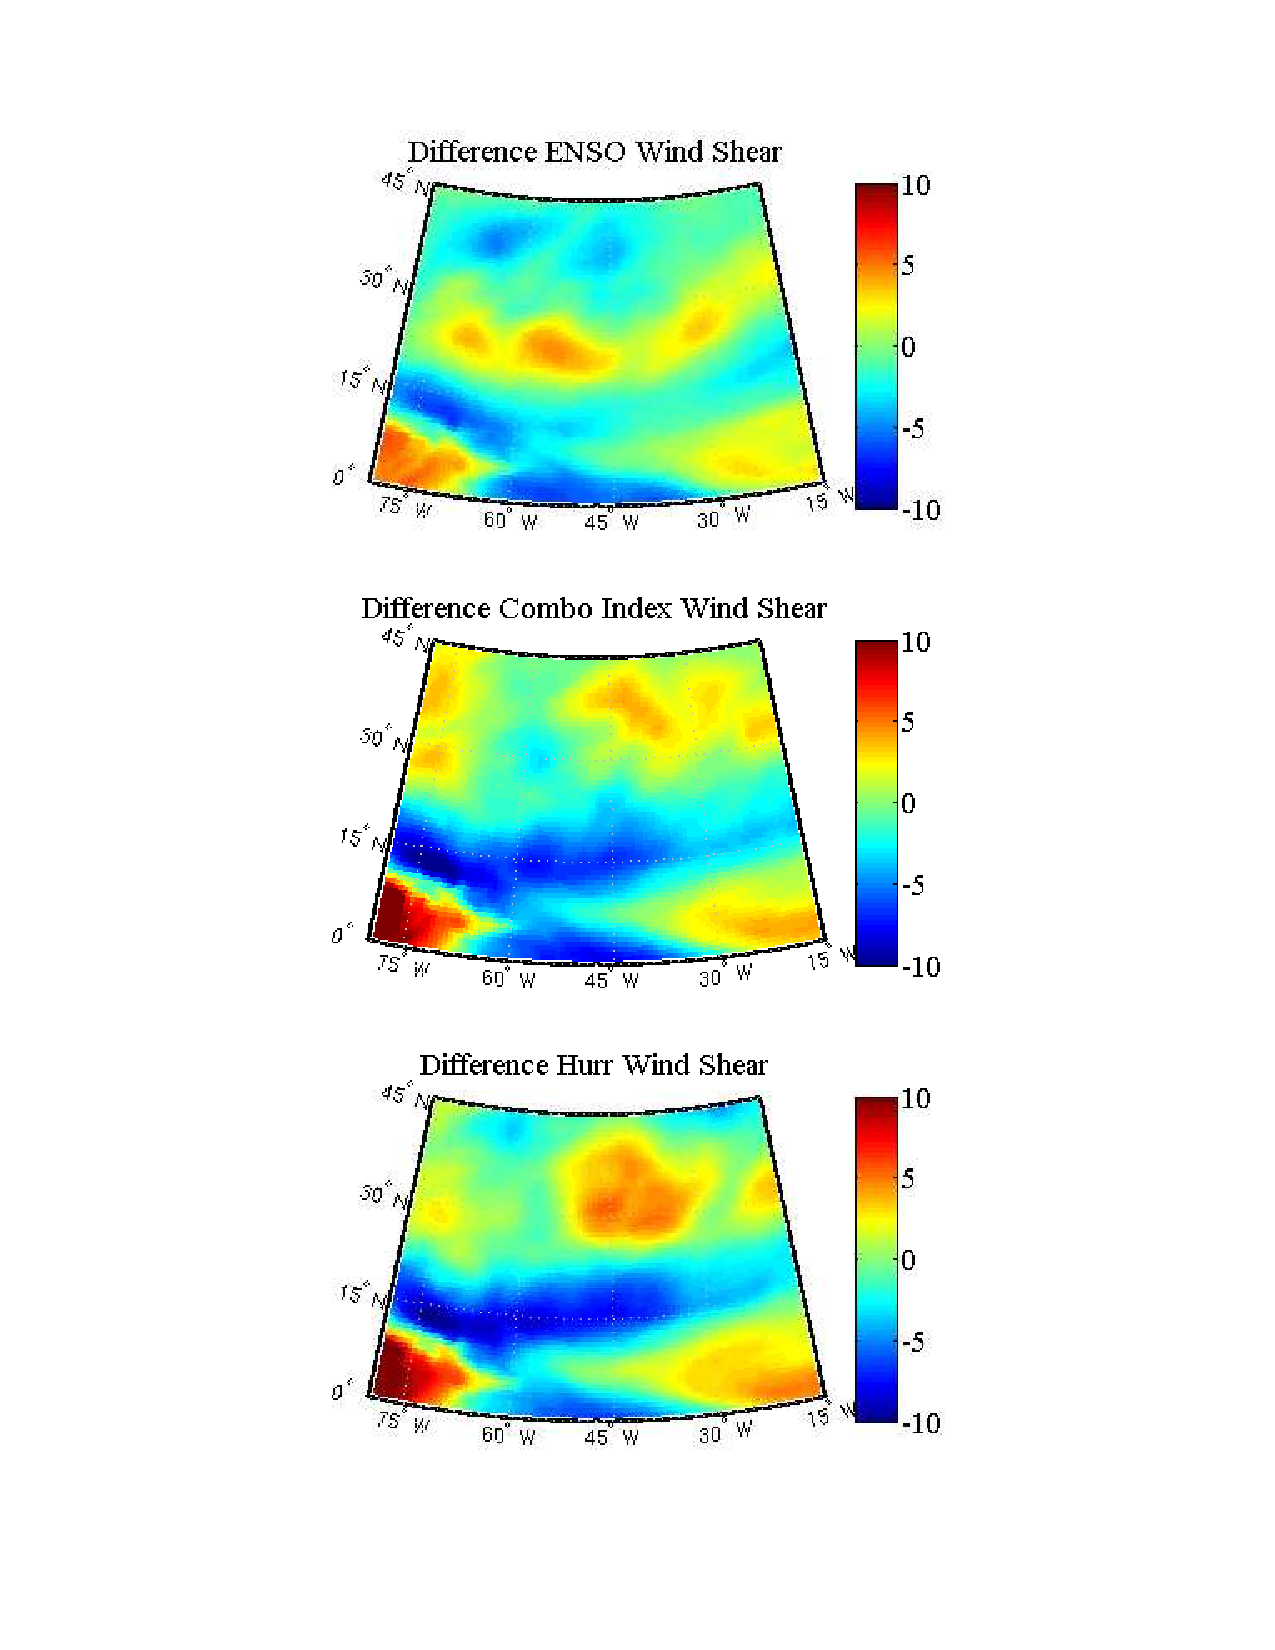
\includegraphics[width=\textwidth]{figures/comboIndex/composites/compareMDRCompositesWindShear.pdf}
\caption{Diff Pressure Composites}
\label{fig:figure21}
\end{minipage}
\hspace{0cm}
\begin{minipage}[b]{0.55\linewidth}
%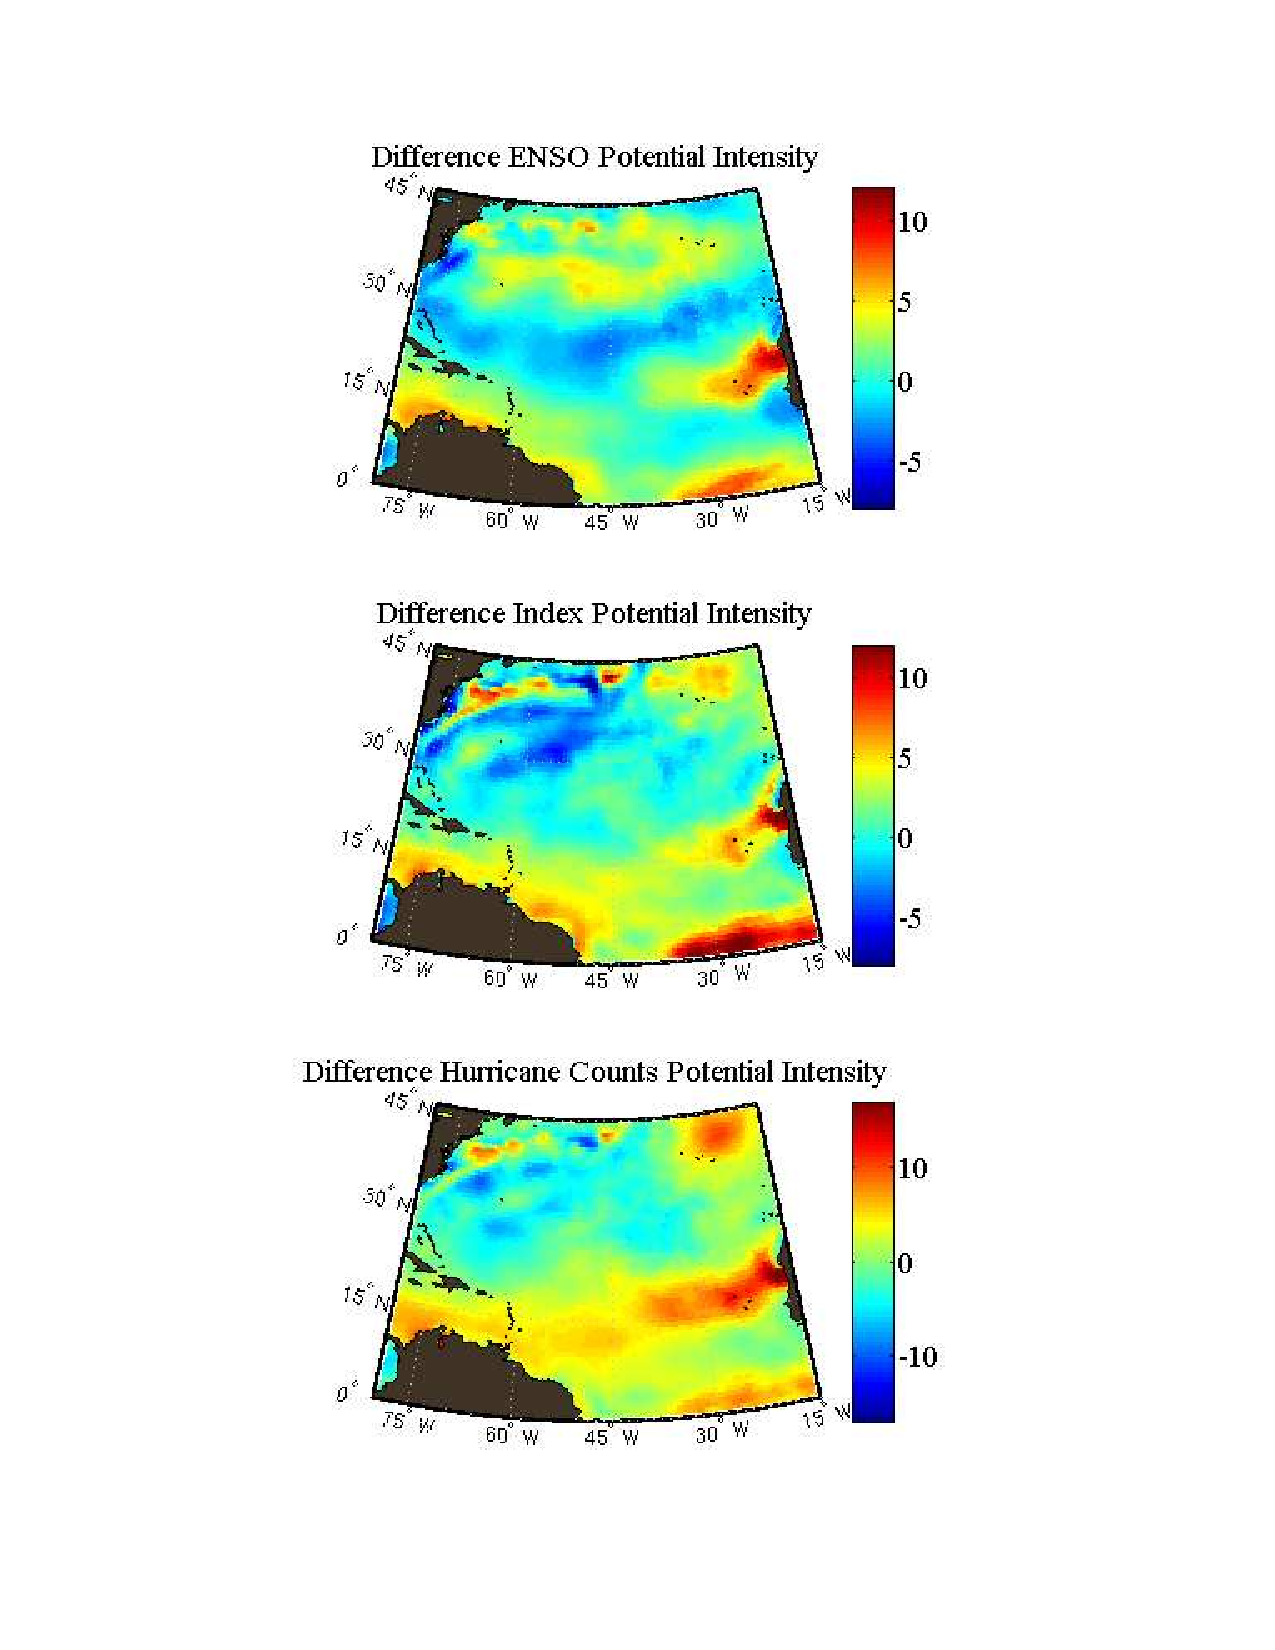
\includegraphics[width=\textwidth]{figures/sensitivityResults/compositeMaps/diffPIAtlanticComposites.pdf}
%\caption{Diff PI Composites}
\label{fig:figure22}
\end{minipage}
\end{figure}

\clearpage
\bibliographystyle{plain}
\bibliography{hurricanes_copy}
\end{document}
